\documentclass[11pt]{article}
\usepackage[margin=1in]{geometry}    
\usepackage{stackengine,graphicx}
\usepackage{caption}
\usepackage{subcaption}
\usepackage{indentfirst}
\usepackage{graphicx}
\usepackage{kbordermatrix}
\usepackage{physics}
\usepackage{mathtools}
\usepackage{listings}
\usepackage{float}
\usepackage{xcolor}
\usepackage{amsmath}
\definecolor{codegreen}{rgb}{0,0.6,0}
\definecolor{codegray}{rgb}{0.3,0.3,0.3}
\definecolor{codepurple}{rgb}{0.58,0,0.82}
\definecolor{backcolour}{rgb}{0.97,0.97,0.97}
\definecolor{mygreen}{RGB}{28,172,0} % color values Red, Green, Blue
\definecolor{mylilas}{RGB}{170,55,241}

\lstset{language=Matlab,%
    basicstyle=\ttfamily,
    breaklines=true,%
    morekeywords={matlab2tikz},
    keywordstyle=\color{blue},%
    morekeywords=[2]{1}, keywordstyle=[2]{\color{black}},
    identifierstyle=\color{black},%
    stringstyle=\color{mylilas},
    commentstyle=\color{mygreen},%
    showstringspaces=false,%without this there will be a symbol in the places where there is a space
    numbers=left,%
    numberstyle={\tiny \color{black}},% size of the numbers
    numbersep=9pt, % this defines how far the numbers are from the text
    emph=[1]{for,end,break},emphstyle=[1]\color{red}, %some words to emphasise
    %emph=[2]{word1,word2}, emphstyle=[2]{style},    
}

\usepackage[superscript,biblabel]{cite}
\usepackage{amsthm, amsmath, amssymb}
\DeclareMathOperator*{\argmin}{\arg\!\min}
\usepackage{setspace}\onehalfspacing
\usepackage[loose,nice]{units}  
\usepackage [english]{babel}
\usepackage{array,booktabs}
\usepackage [autostyle, english = american]{csquotes}
\MakeOuterQuote{"}
\title{Homework 6 \large \\ CAAM 28200: Dynamical Systems with Applications}
\author{Kameel Khabaz}
\date{\today}
\frenchspacing     
\begin{document}
\maketitle

\section*{Simulation Exercises (Lorenz)}
Here I simulate the Lorenz system for $\sigma = 10$, $ b = 8/3$, and $r$ varying from just below $r_H$ to just above $r_H$. The resulting trajectories starting from $x_0$ near $C_+ = <\sqrt{b(r-1)},\sqrt{b(r-1)}, r-1>$ are shown below. We see here in the top row that when $r < r_H$, the trajectory spirals towards the stable fixed point $C_+$. We can also tell this when we look at a plot of one of the coordinates versus time (on the left of the next figure). We see that while there is transient chaos at this value of $r$, the solution eventually damps down to equilibrium. On the other hand, when $r>r_H$, as on the bottom row, we clearly see chaotic solutions and we see the shape of the strange attractor. When we look at the plot of $y$ vs. $t$, we clearly see that the solution for $r > r_H$ (on the right) is aperiodic. 
\begin{figure}[h]
\centering
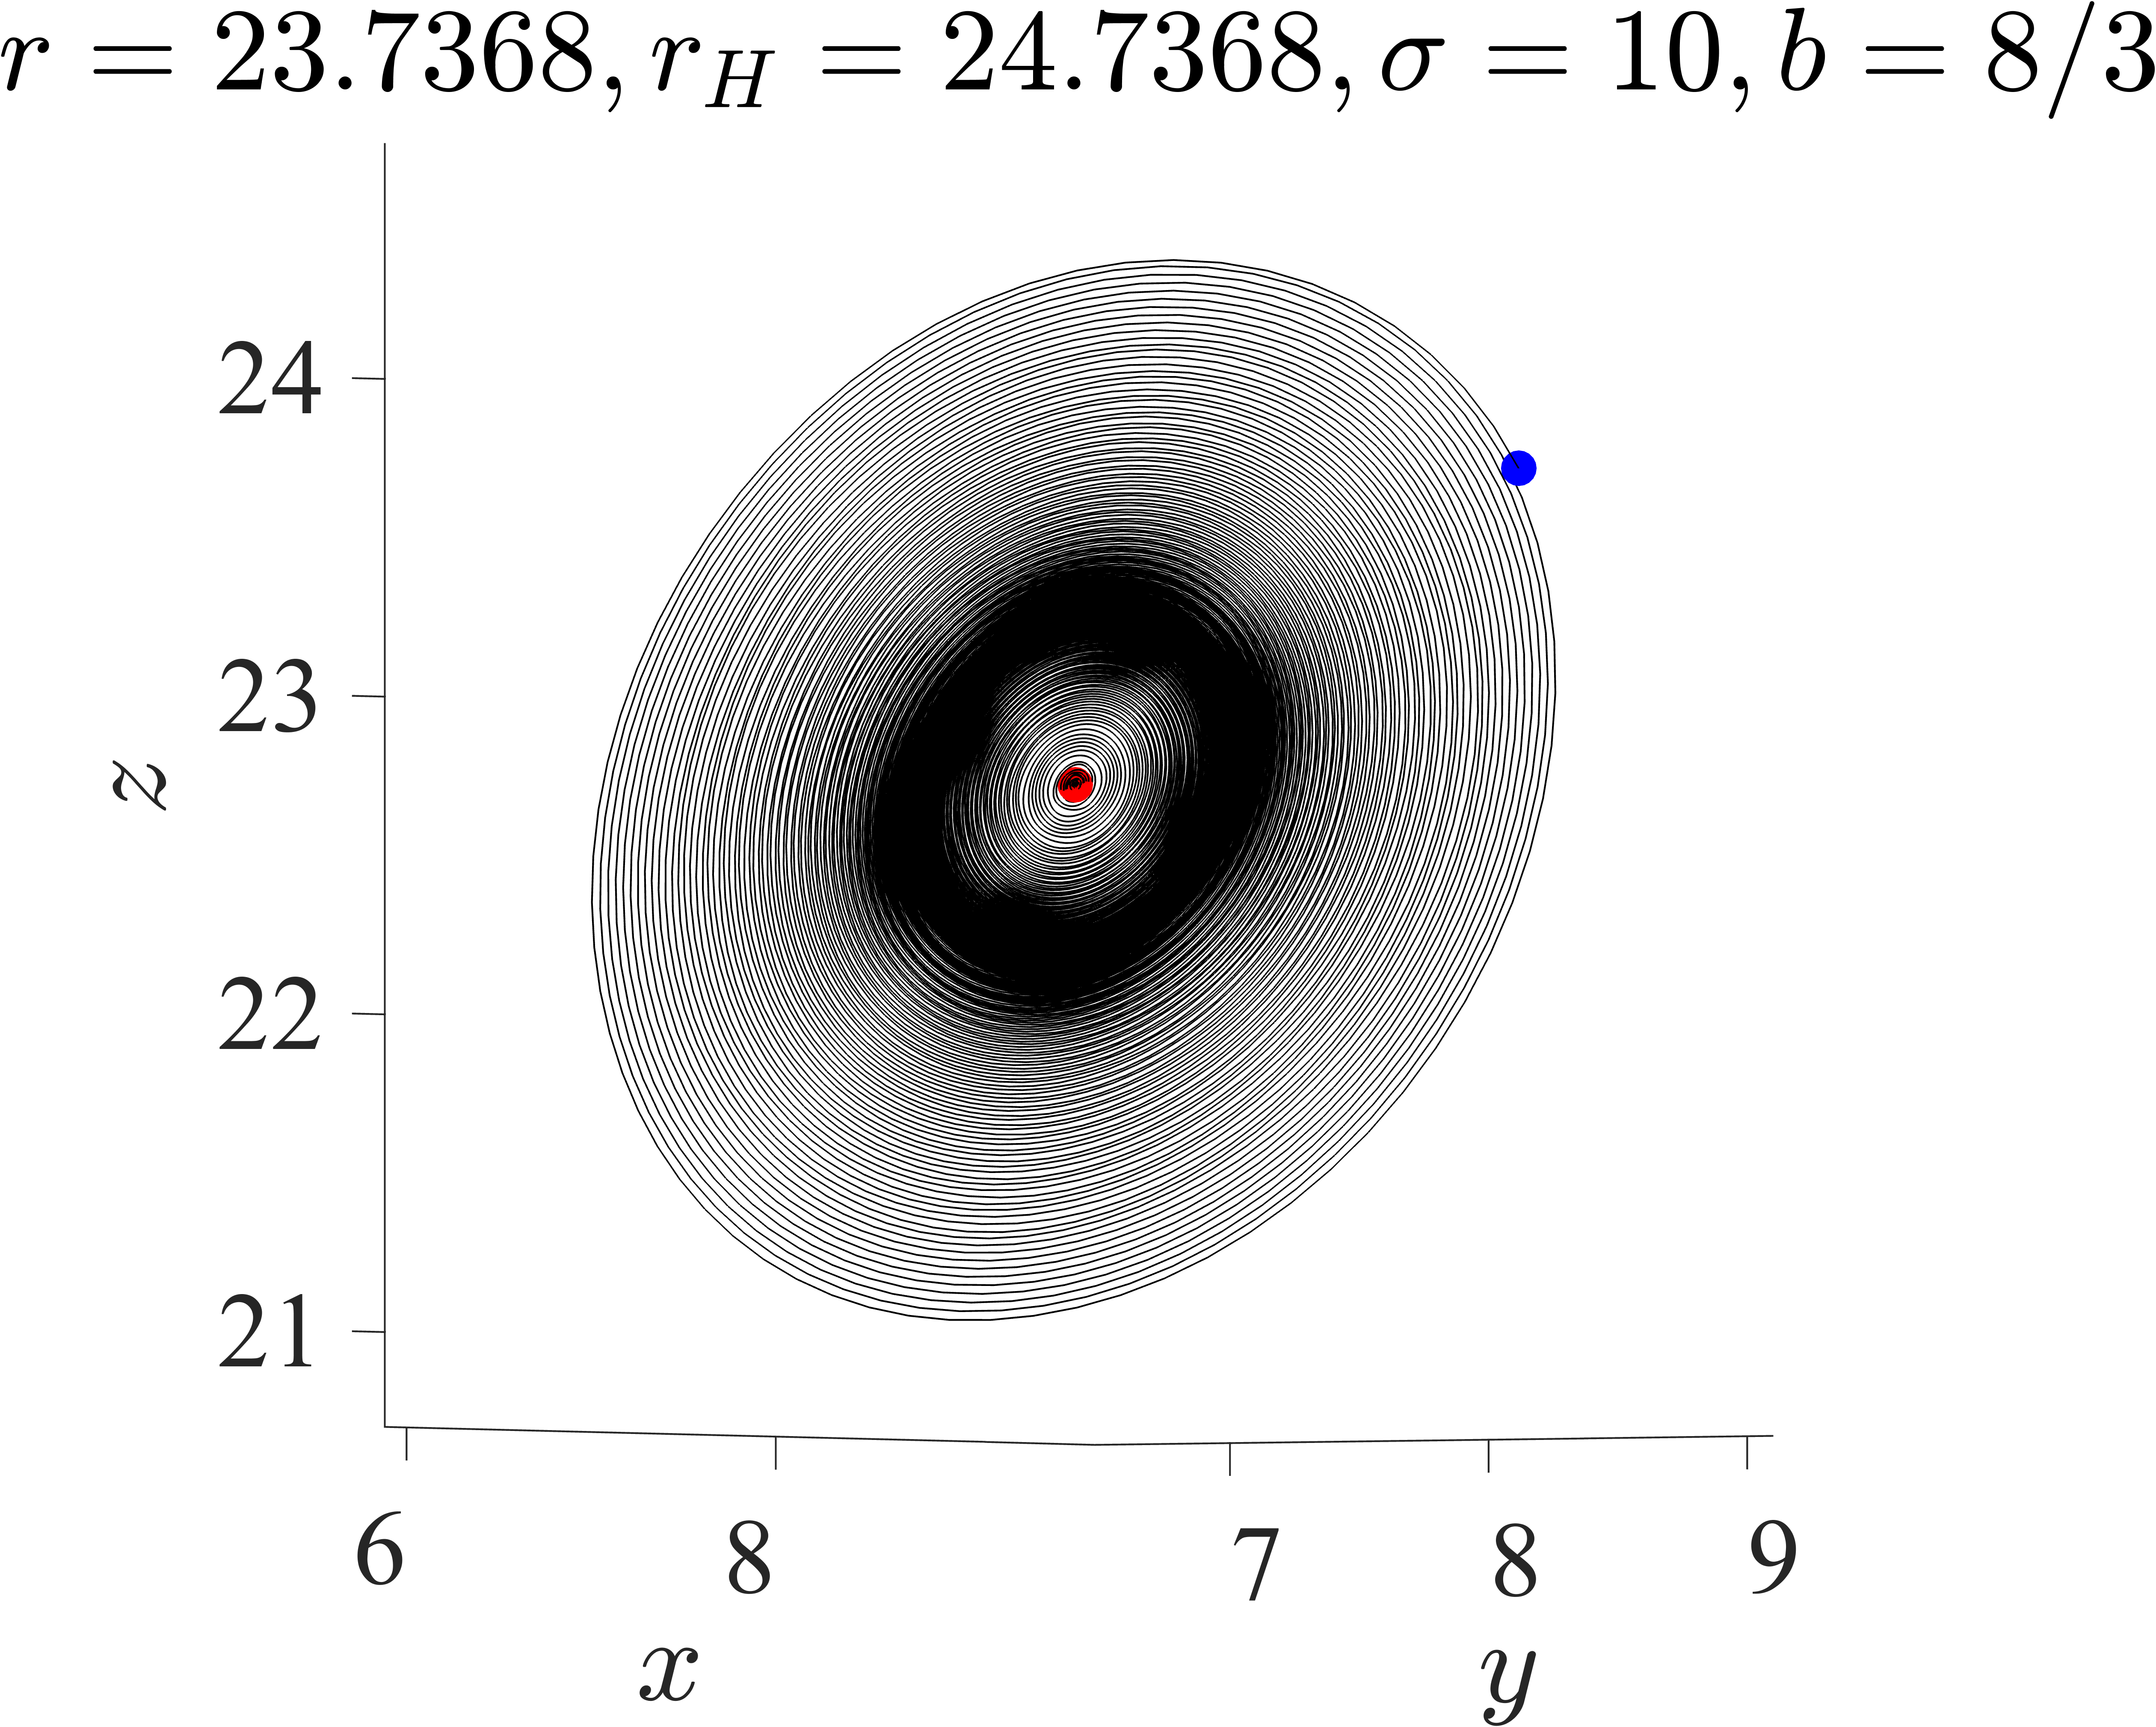
\includegraphics[width=9cm]{Lorenz_r23.7368.png}
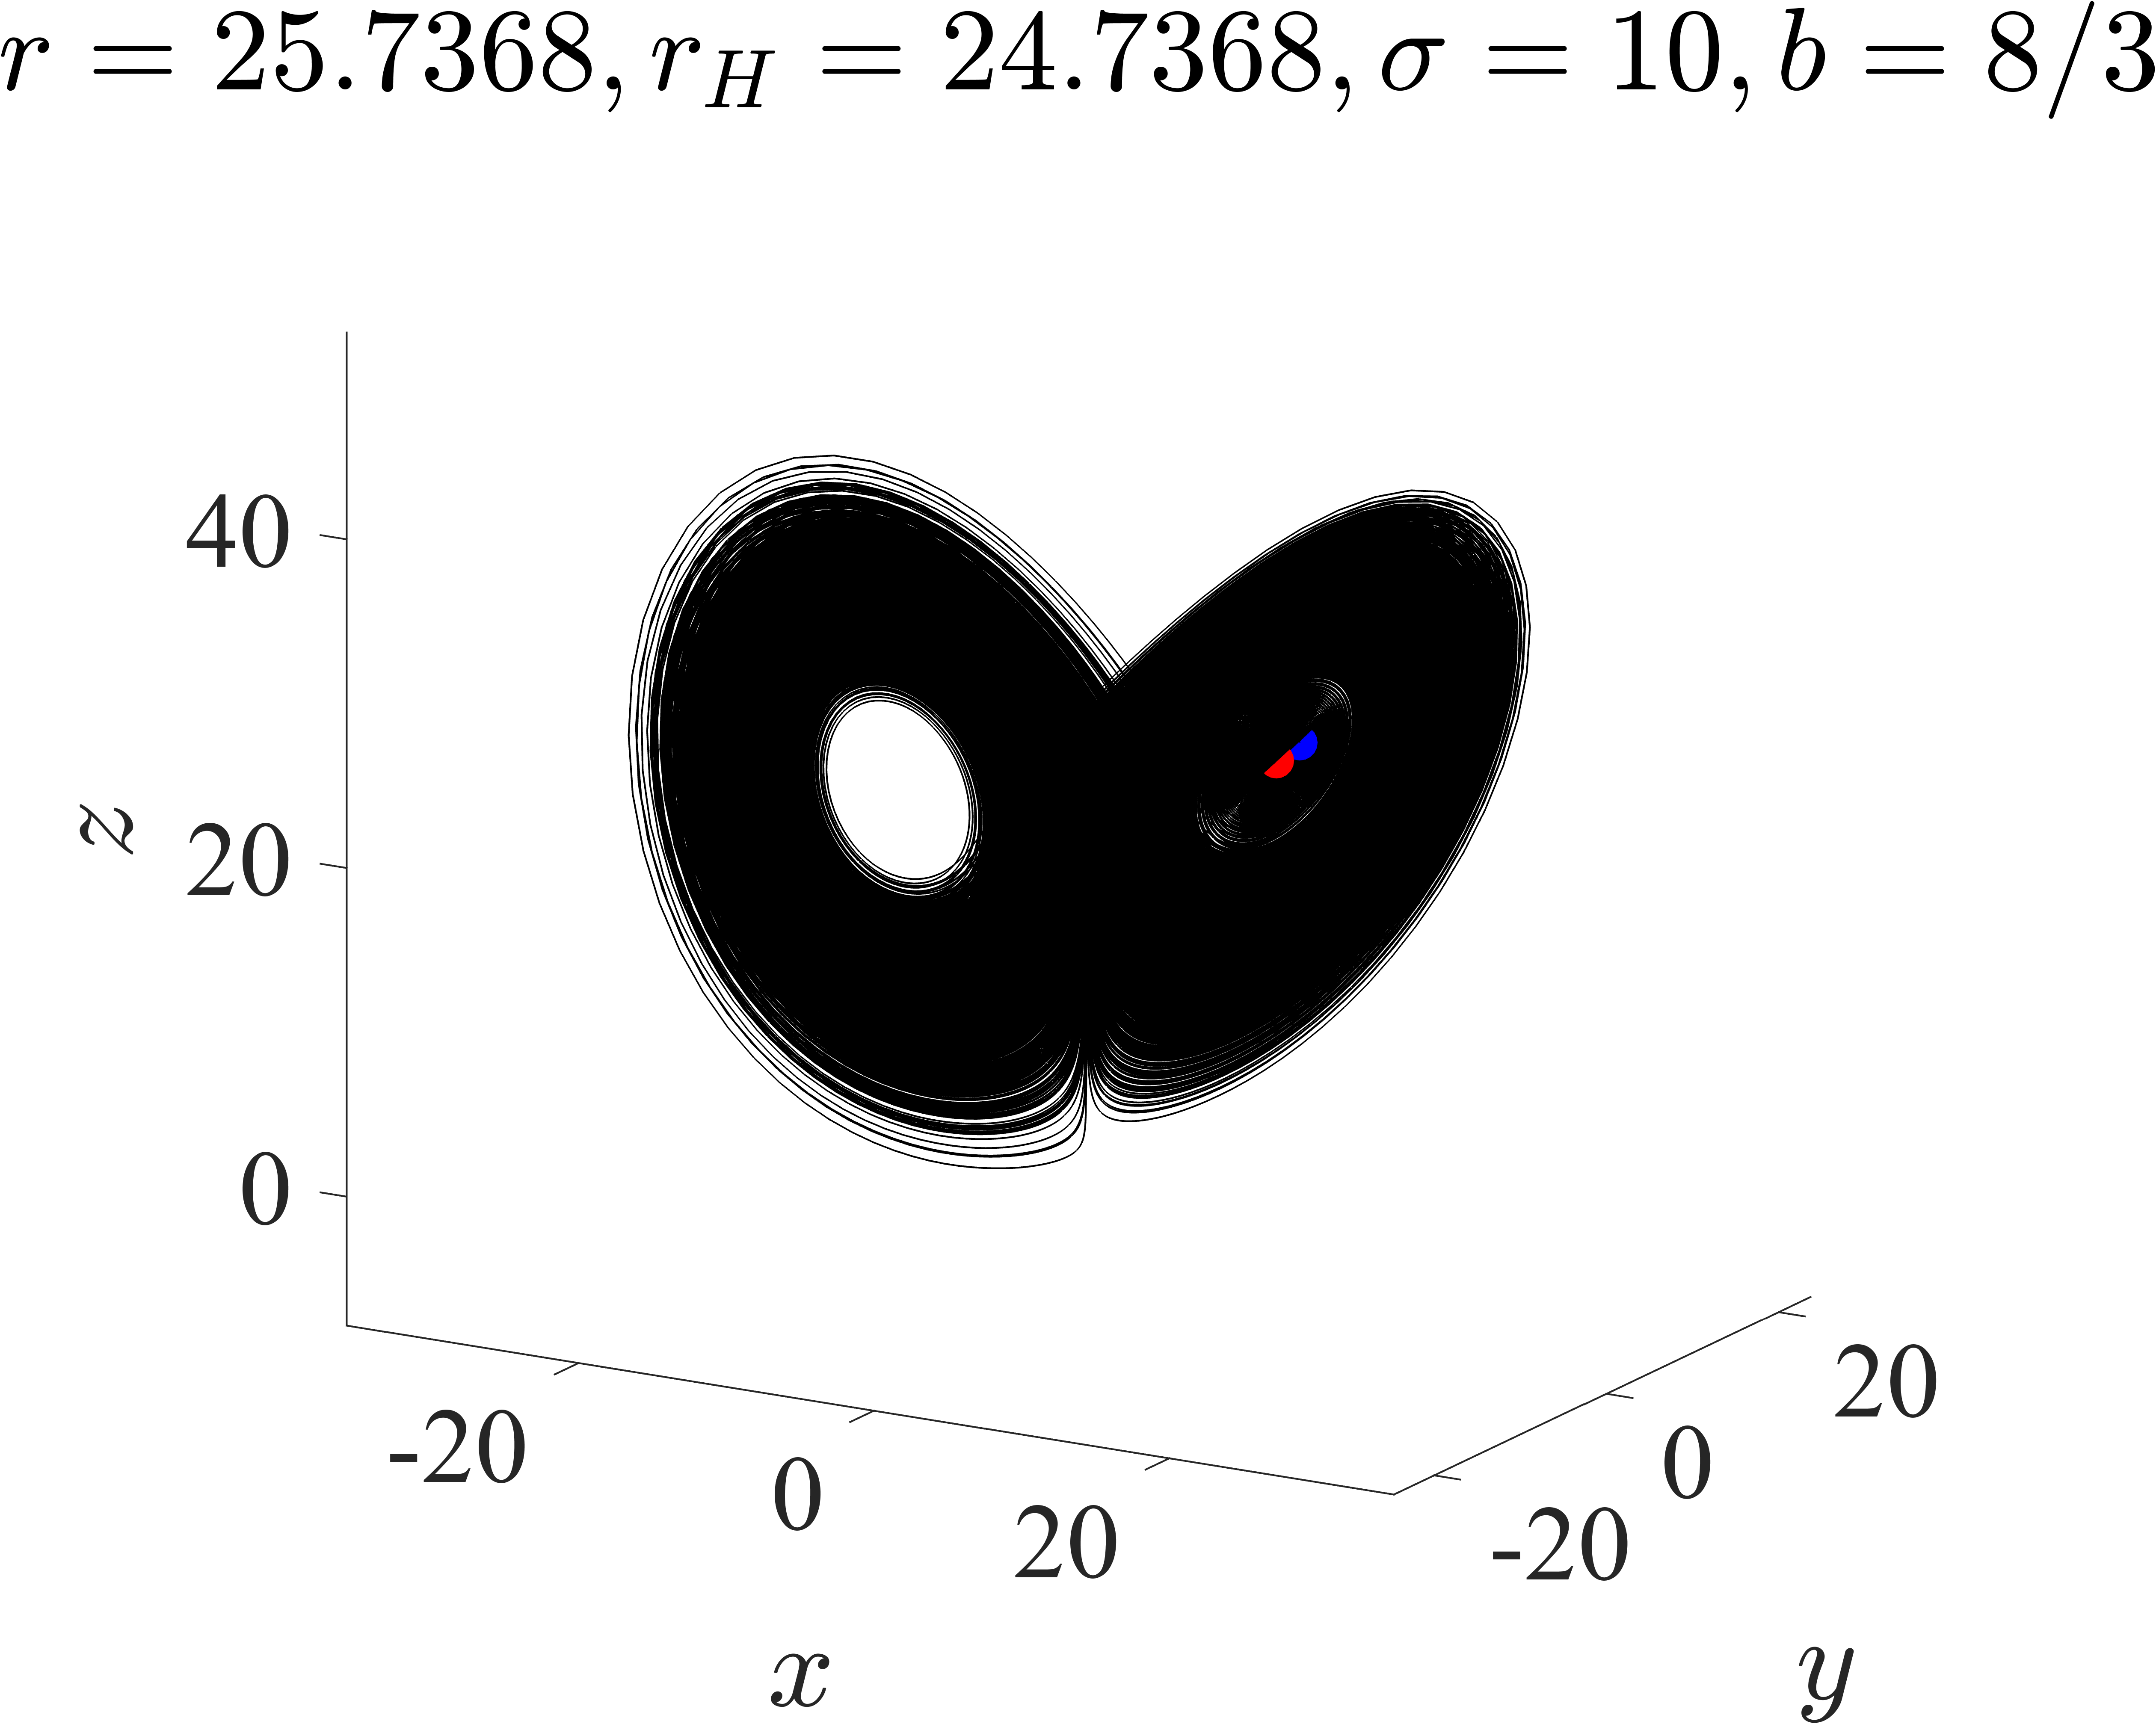
\includegraphics[width=8cm]{Lorenz_r25.7368.png}
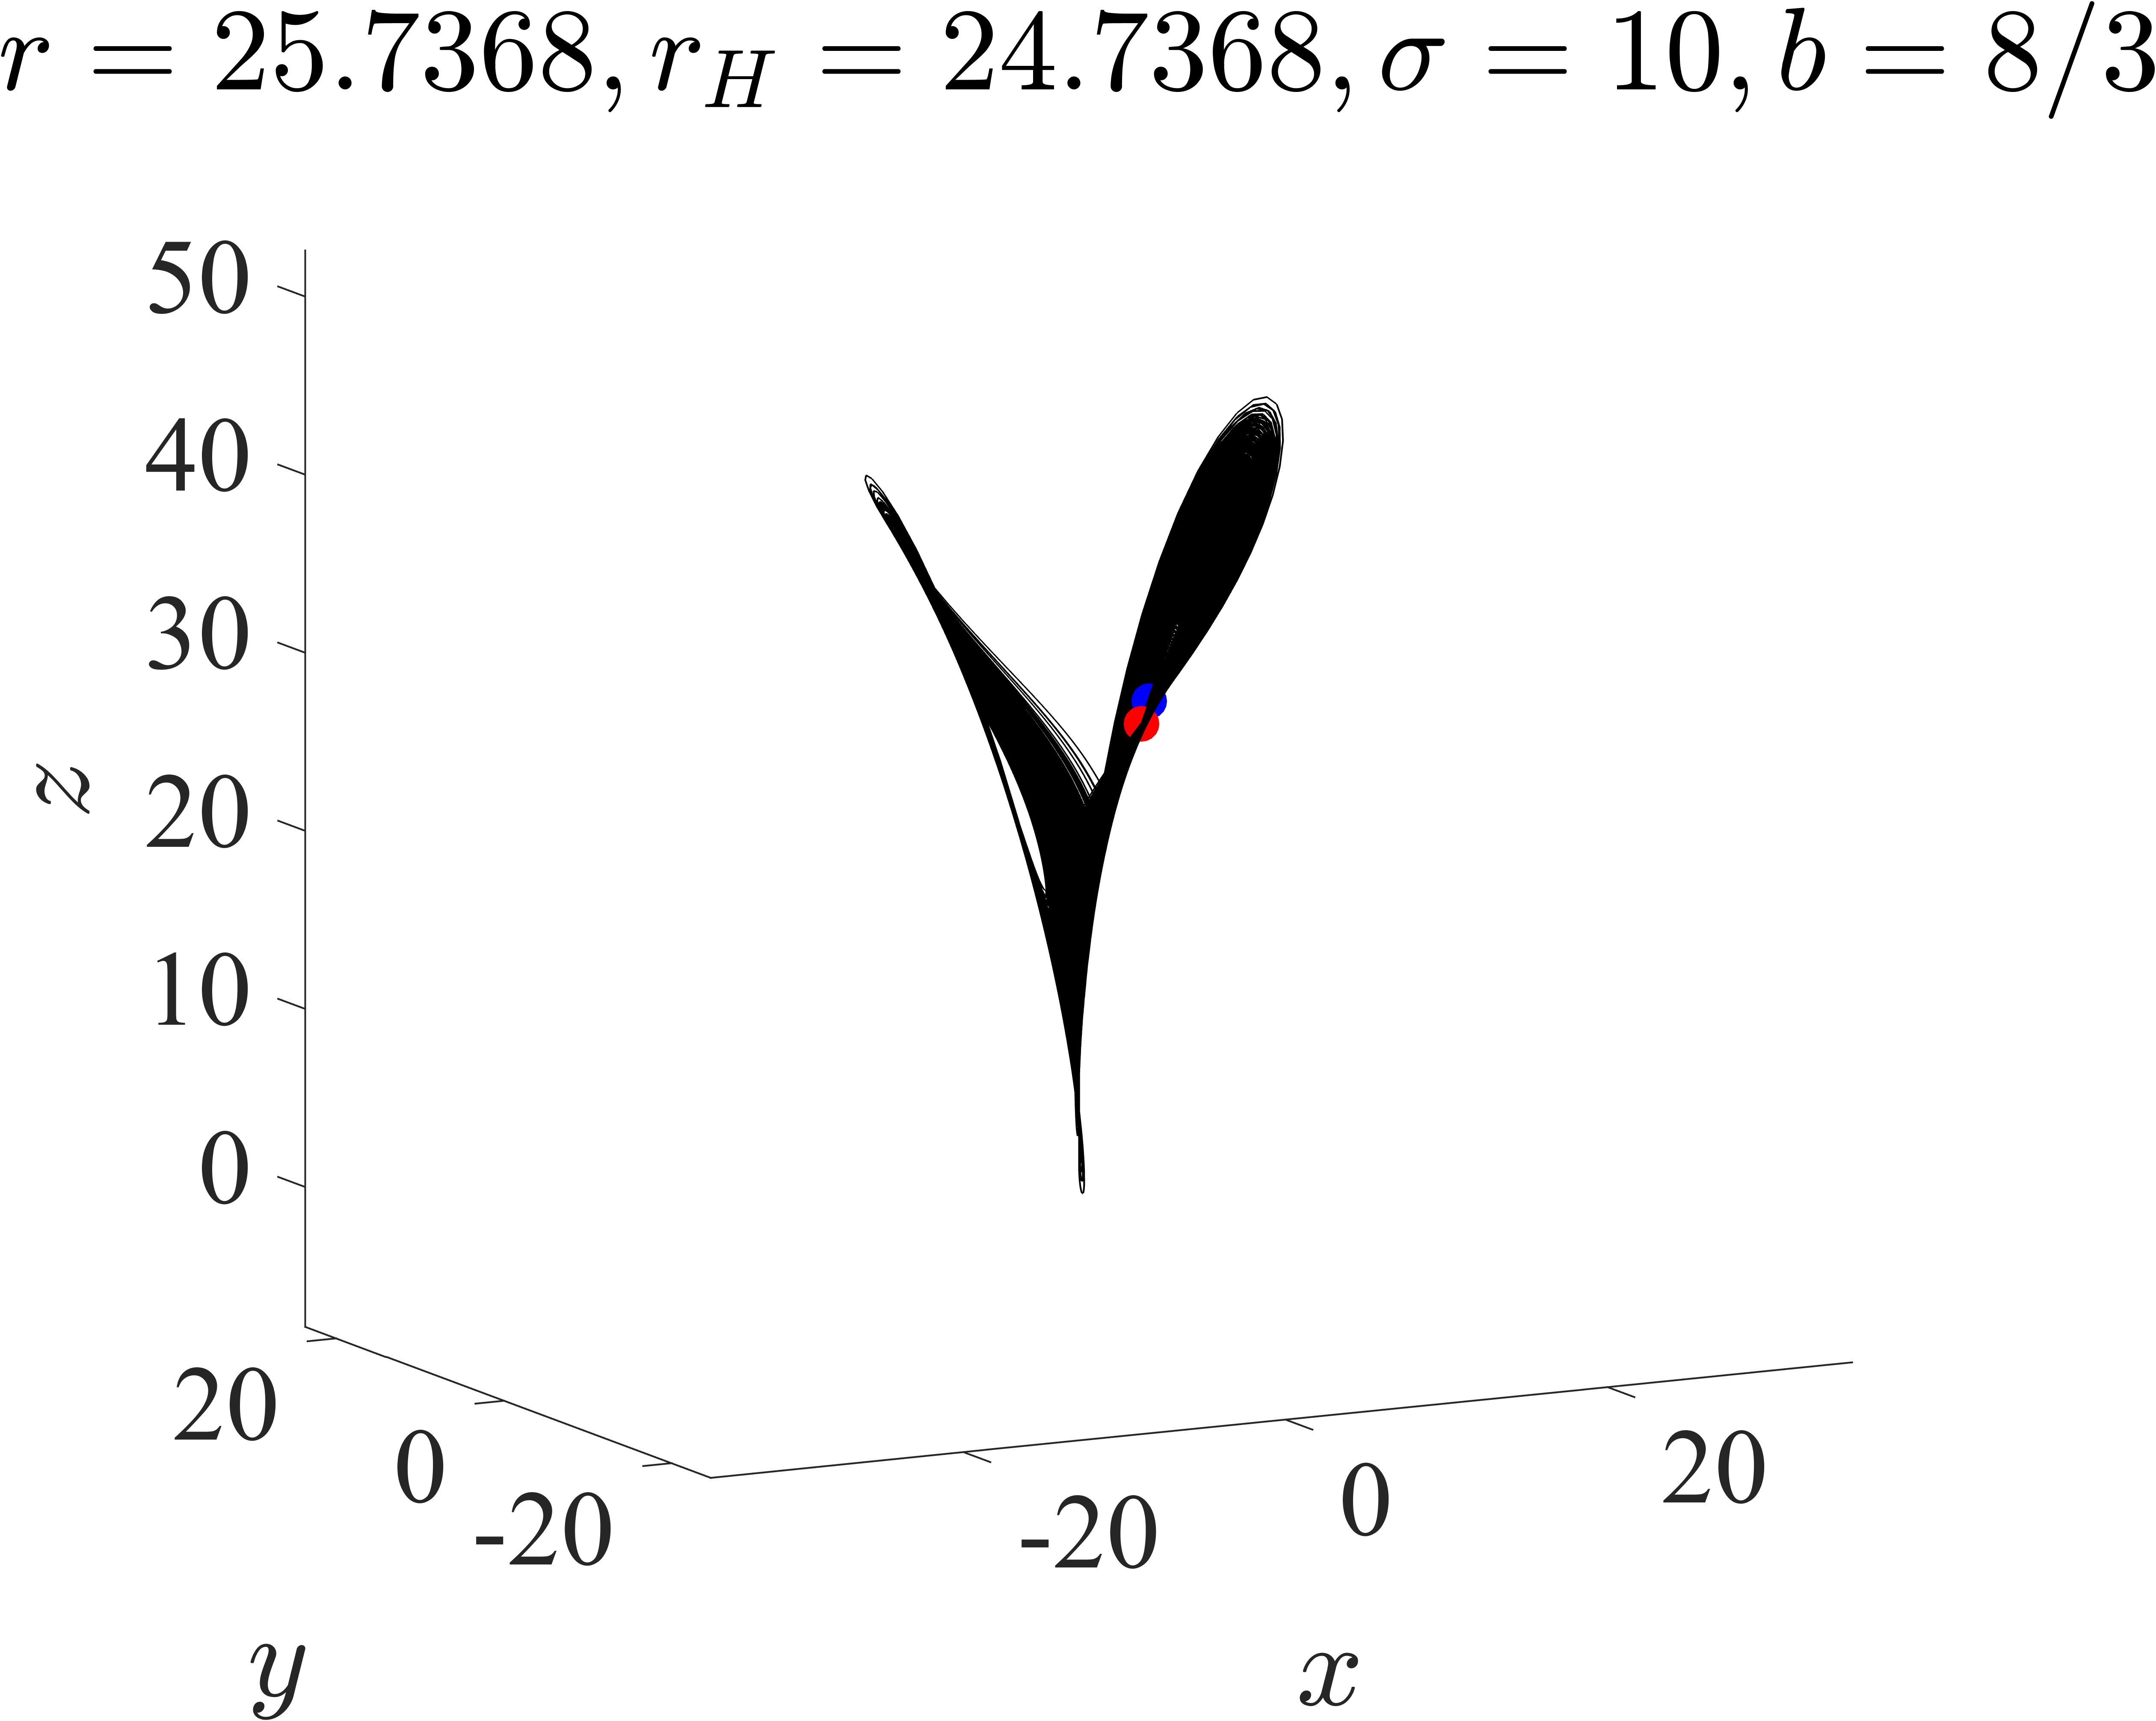
\includegraphics[width=8cm]{Lorenz_r25.7368_2.png}
\caption{Lorenz Attractor}
\end{figure}

\begin{figure}[h]
\centering
\subfloat{a. $r < r_H$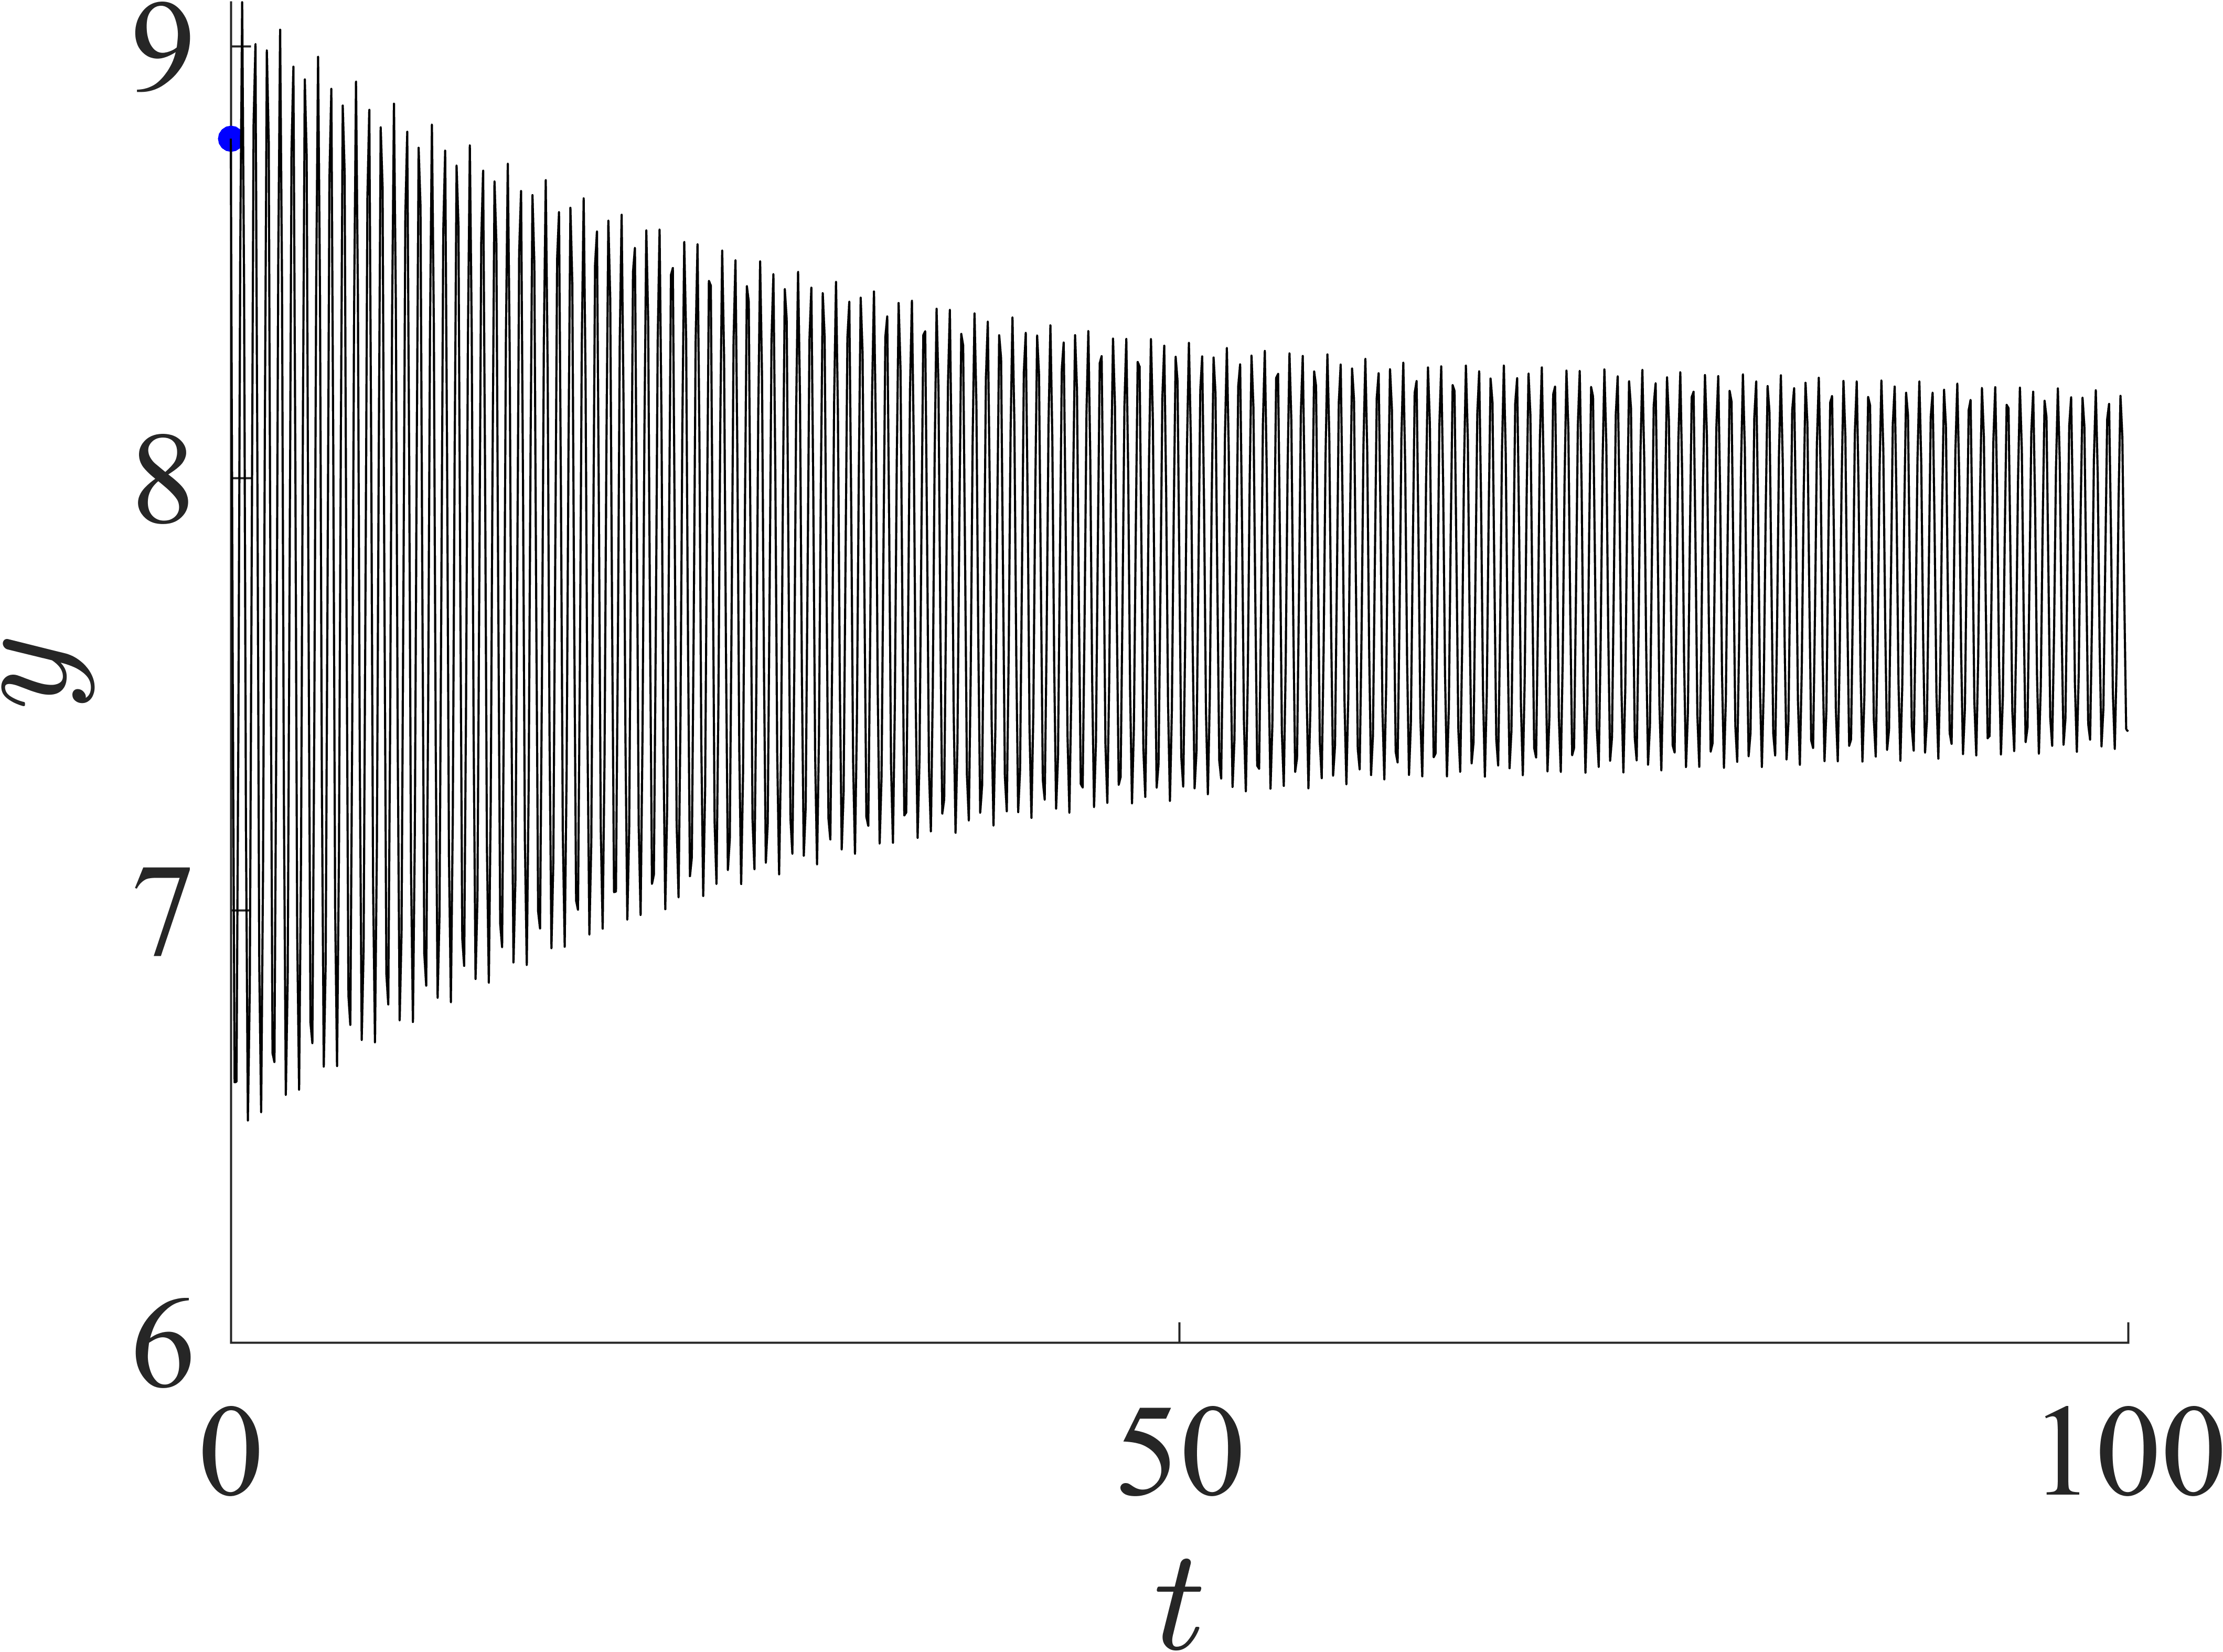
\includegraphics[width=7cm]{Lorenz_r23.7368y.png}}
\subfloat{b. $r > r_H$ 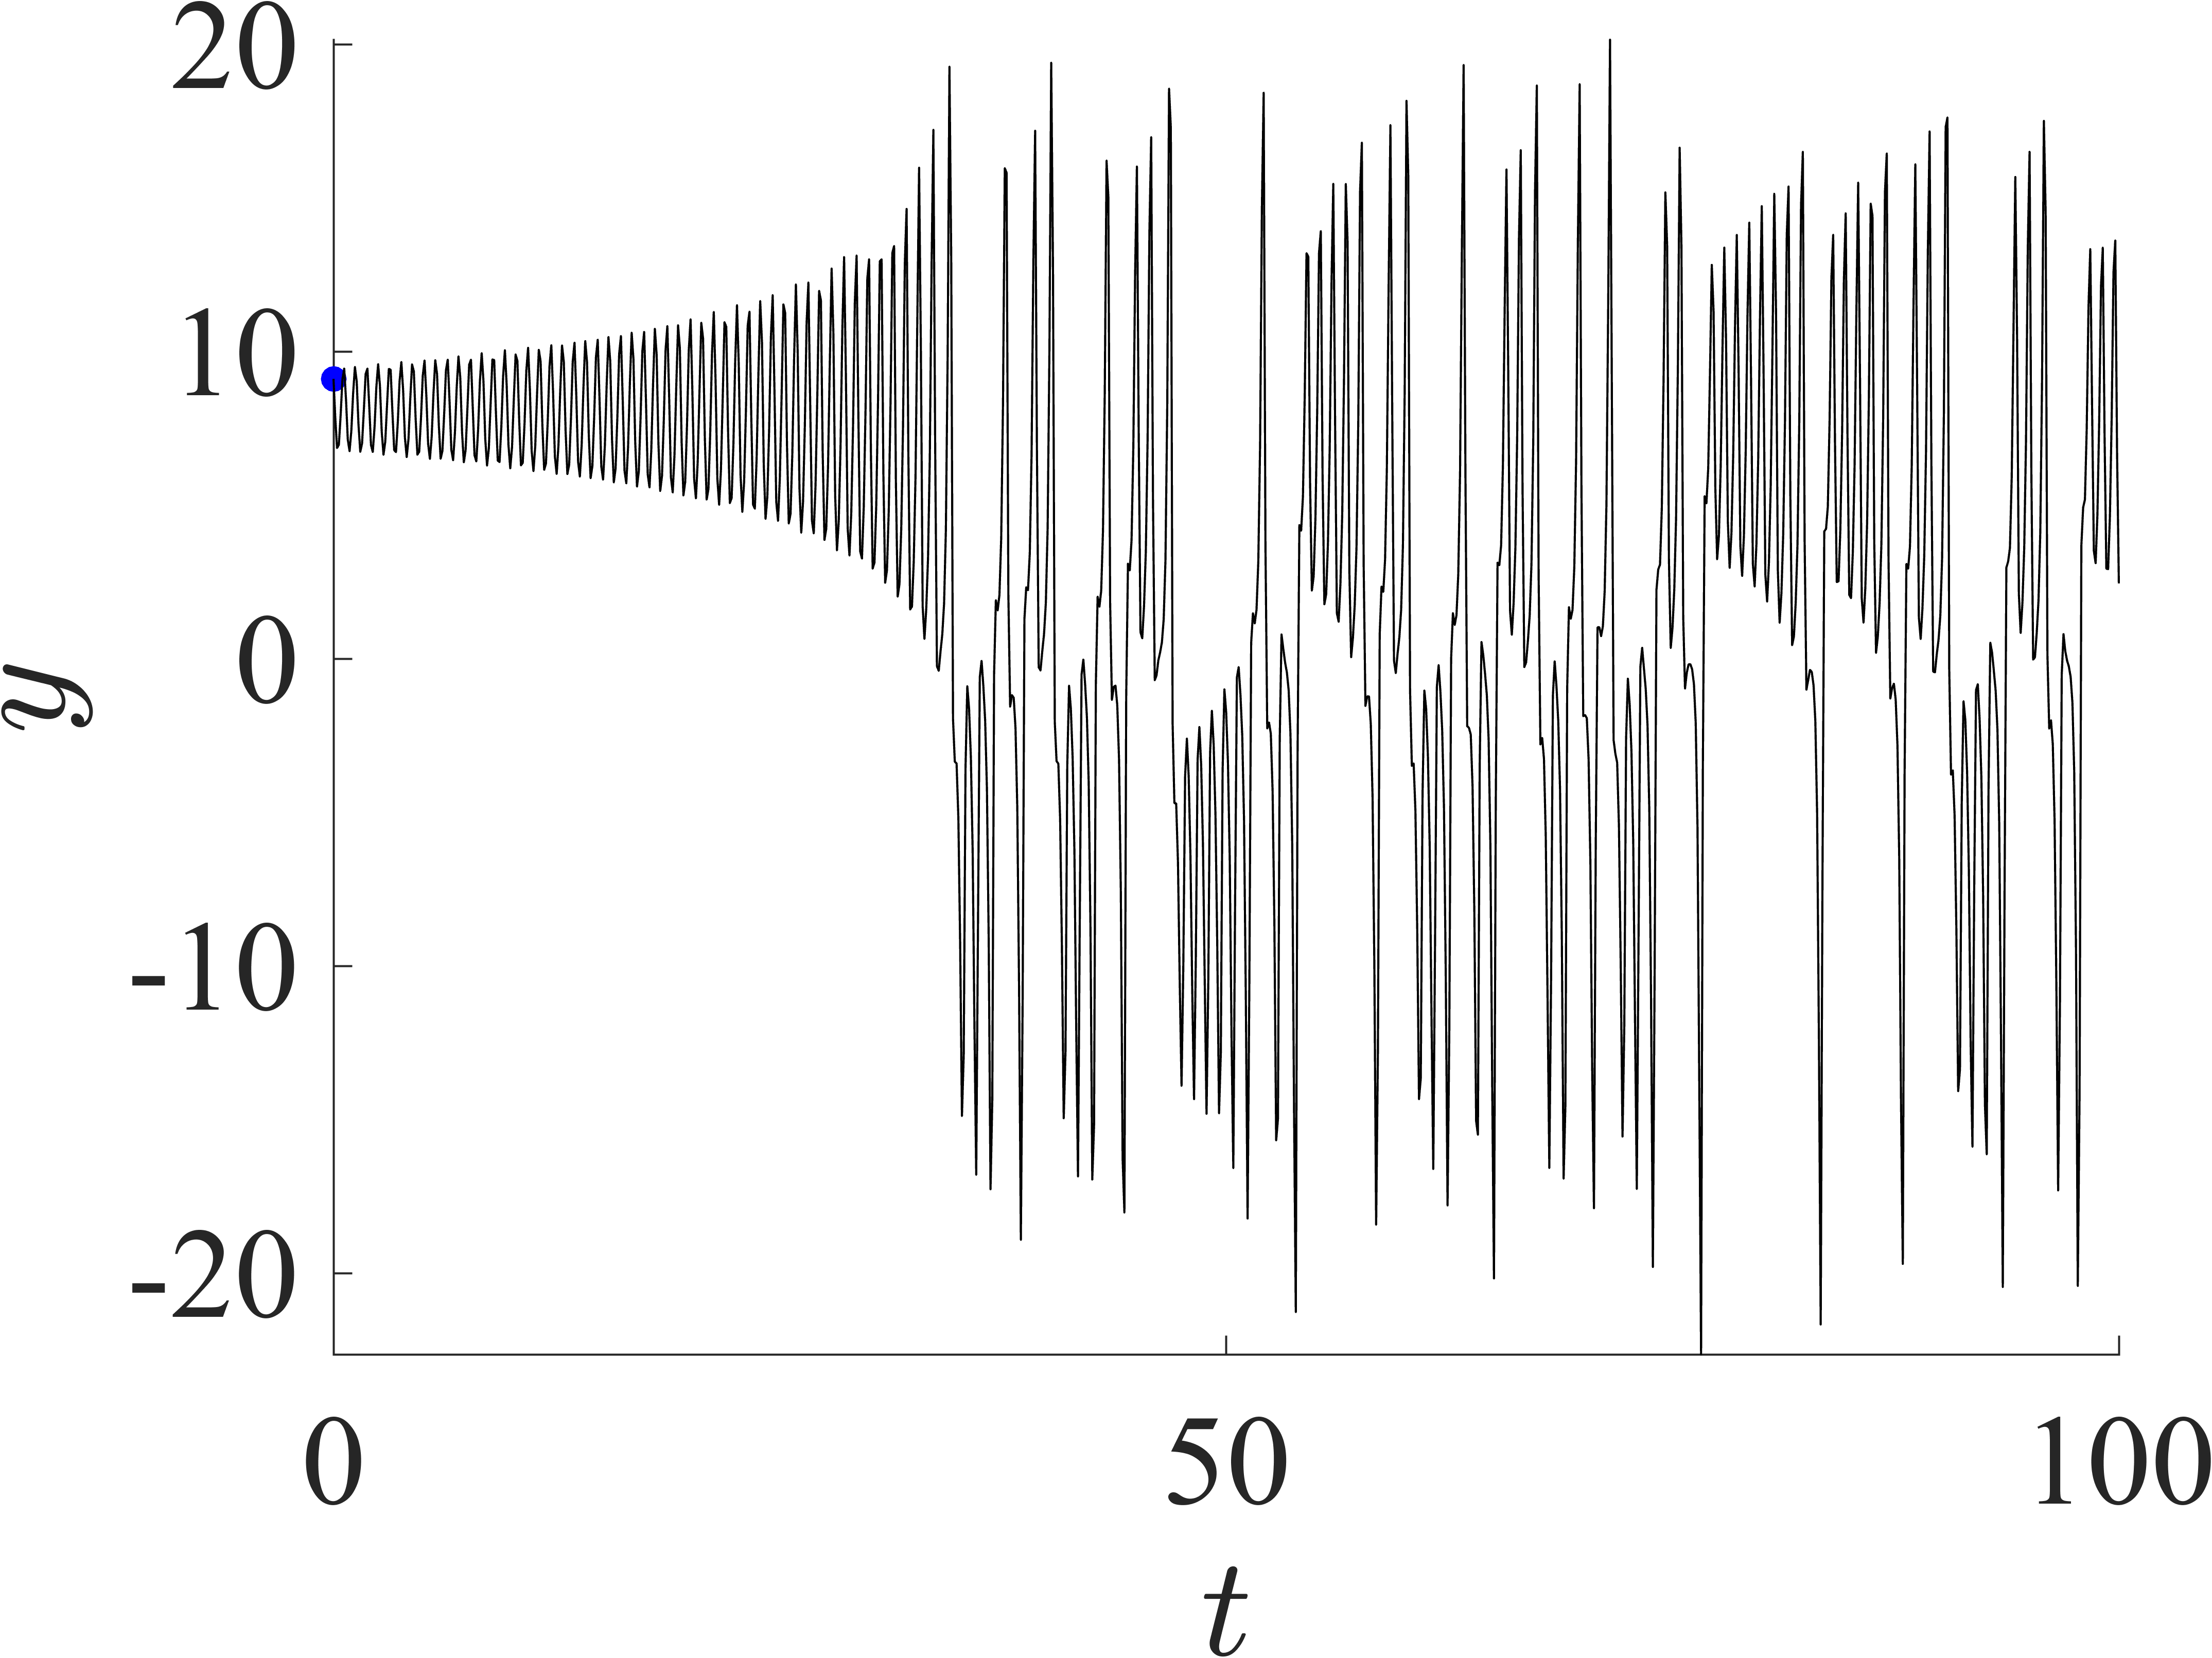
\includegraphics[width=7cm]{Lorenz_r25.7368y.png}}
\caption{Lorenz Attractor}
\end{figure}

\clearpage
Now we start two trajectories with initial conditions $x_0$ and $y_0 = x_0 + \delta$ near $x_0$. We see the result here, in which one starts at the blue dot and the other starts at the green dot. In this figure, we see that they must both be contained within the strange attractor over long time scales, but we cannot easily compare the trajectories in 3D.
\begin{figure}[h]
\centering
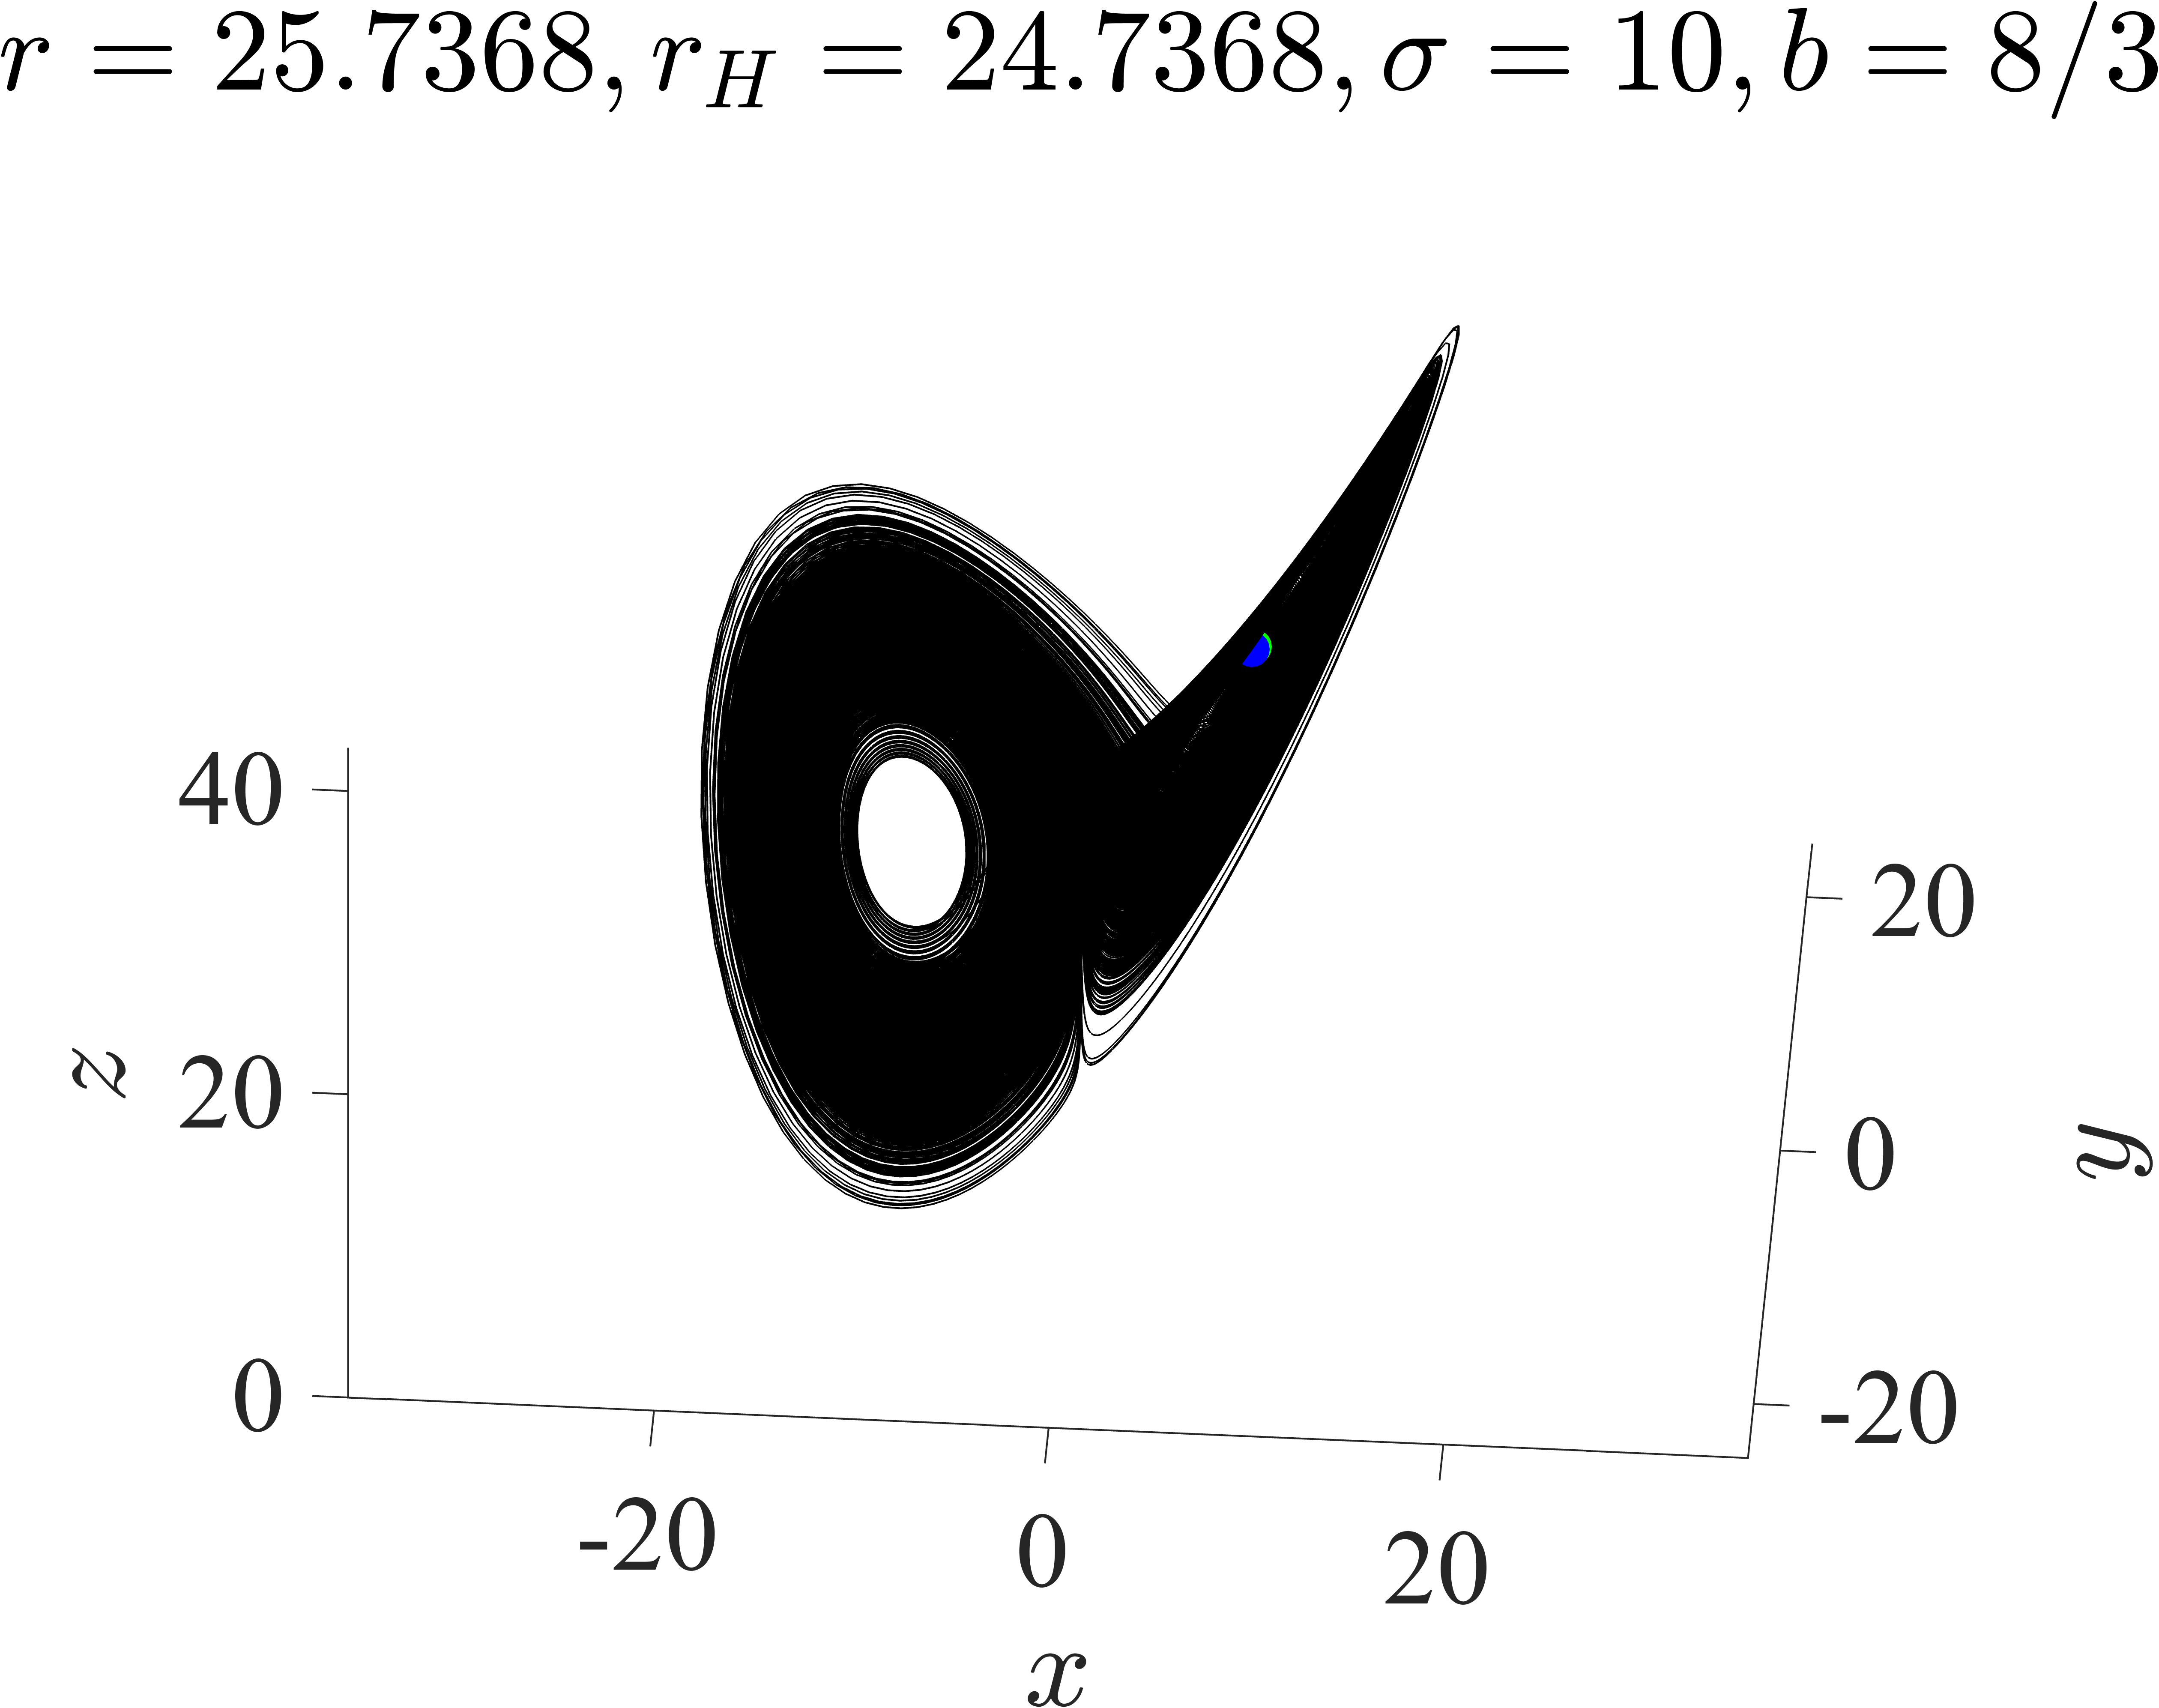
\includegraphics[width=8cm]{Lorenz_r25.73682_trajectories.png}
\caption{Lorenz Attractor: Two Trajectories}
\end{figure}

So, I plot the natural logarithm of the relative discrepancy between the trajectories $\ln(\frac{||y(t) - x(t)||}{||\delta||})$ versus time. The plot is shown on the next page. We see here that regardless of $\delta$, the relative discrepancy between the trajectory rapidly increases over time until it reaches a steady value when the two trajectories are mixed (operating relatively independently). The initial phase of exponential increase demonstrates the sensitive dependence on initial conditions of the Lorenz system, and the latter phase tells us that the solution for the Lorenz system is bounded to the order of the diameter of the strange attractor. We see that as $\delta$ decreases, the time range for exponential growth (which I zoom in on in the right panel) increases. So as the initial separation gets smaller, it takes longer and longer for the two trajectories to separate to the point where they operate independently.

When I found the growth rate in the log of the relative discrepancy, I was able to estimate the Lyapanov exponent. We know $||\delta(t)|| \approx ||\delta_0||e^{\lambda  t}$, which implies $\ln ||\delta(t)|| \approx \lambda t + \ln || \delta_0 ||$. So, on the right panel, I calculate this linear fit and find that $\lambda$ is around $0.03$. We do see, however, that the value of $\lambda$ varies slightly with the initial discrepancy. This $\lambda \approx 0.03 $ is the largest Lyapanov exponent. 

Based on this fit, we can calculate the time horizon before which predictions break down. We know that $t_{horizon} \approx O(\frac{1}{\lambda} \ln \frac{a}{\delta_0})$. So, we predict that starting from $\delta = 10^{-6}$, the time that it takes for the discrepancy is greater than $10^{-1}$ is 
 $$t_{horizon} \approx O(\frac{1}{\lambda} \ln \frac{a}{\delta_0}) = \frac{1}{0.03} \ln \frac{10^{-1}}{10^{-6}} = 384 s$$
If we reduce our original measurement error dramatically such that $\delta = 10^{-9}$, then we find that the new time horizon is 
 $$t_{horizon} \approx O(\frac{1}{\lambda} \ln \frac{a}{\delta_0}) = \frac{1}{0.03} \ln \frac{10^{-1}}{10^{-9}} = 614 s$$
 Thus, the new time horizon is only $1.6$ times the old time horizon, or $60\%$ longer. This minimal improvement in prediction capabilities given much higher measurement precision demonstrates the challenge of predicting chaotic systems.
 
 
\begin{figure}[h]
\centering
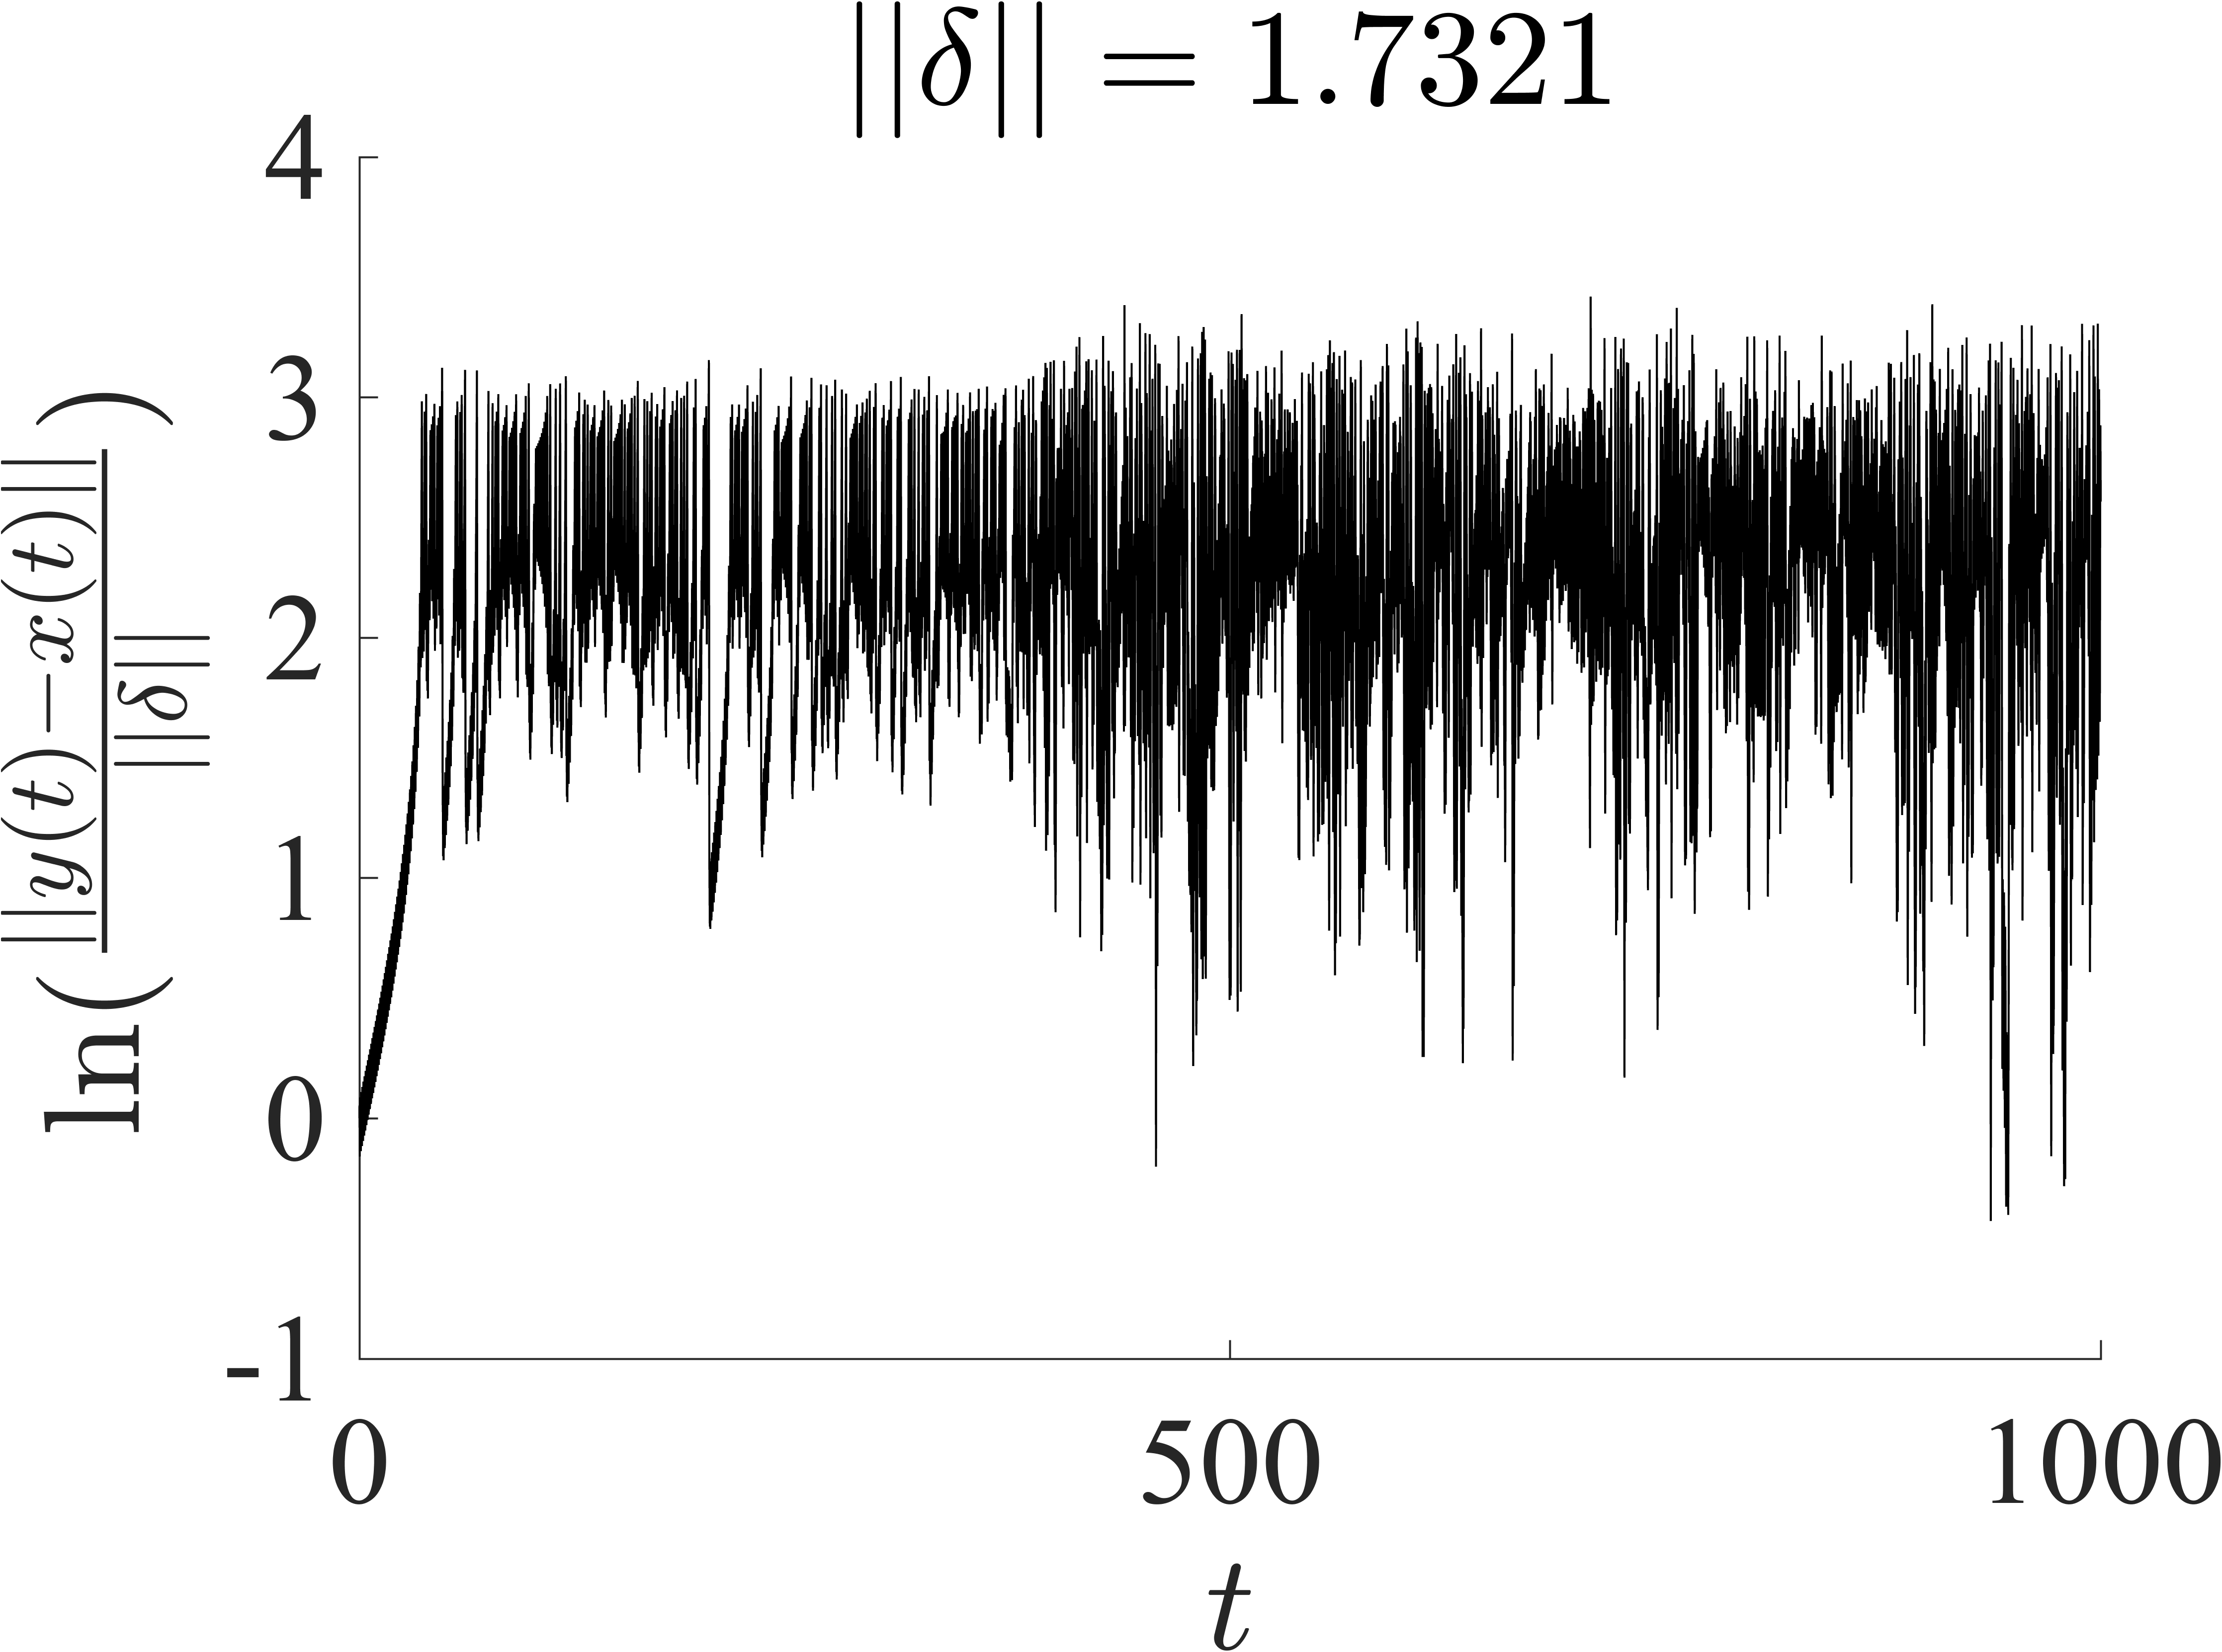
\includegraphics[width=8cm]{Lorenz_r25.73682_trajectories_discp_delta4.png}
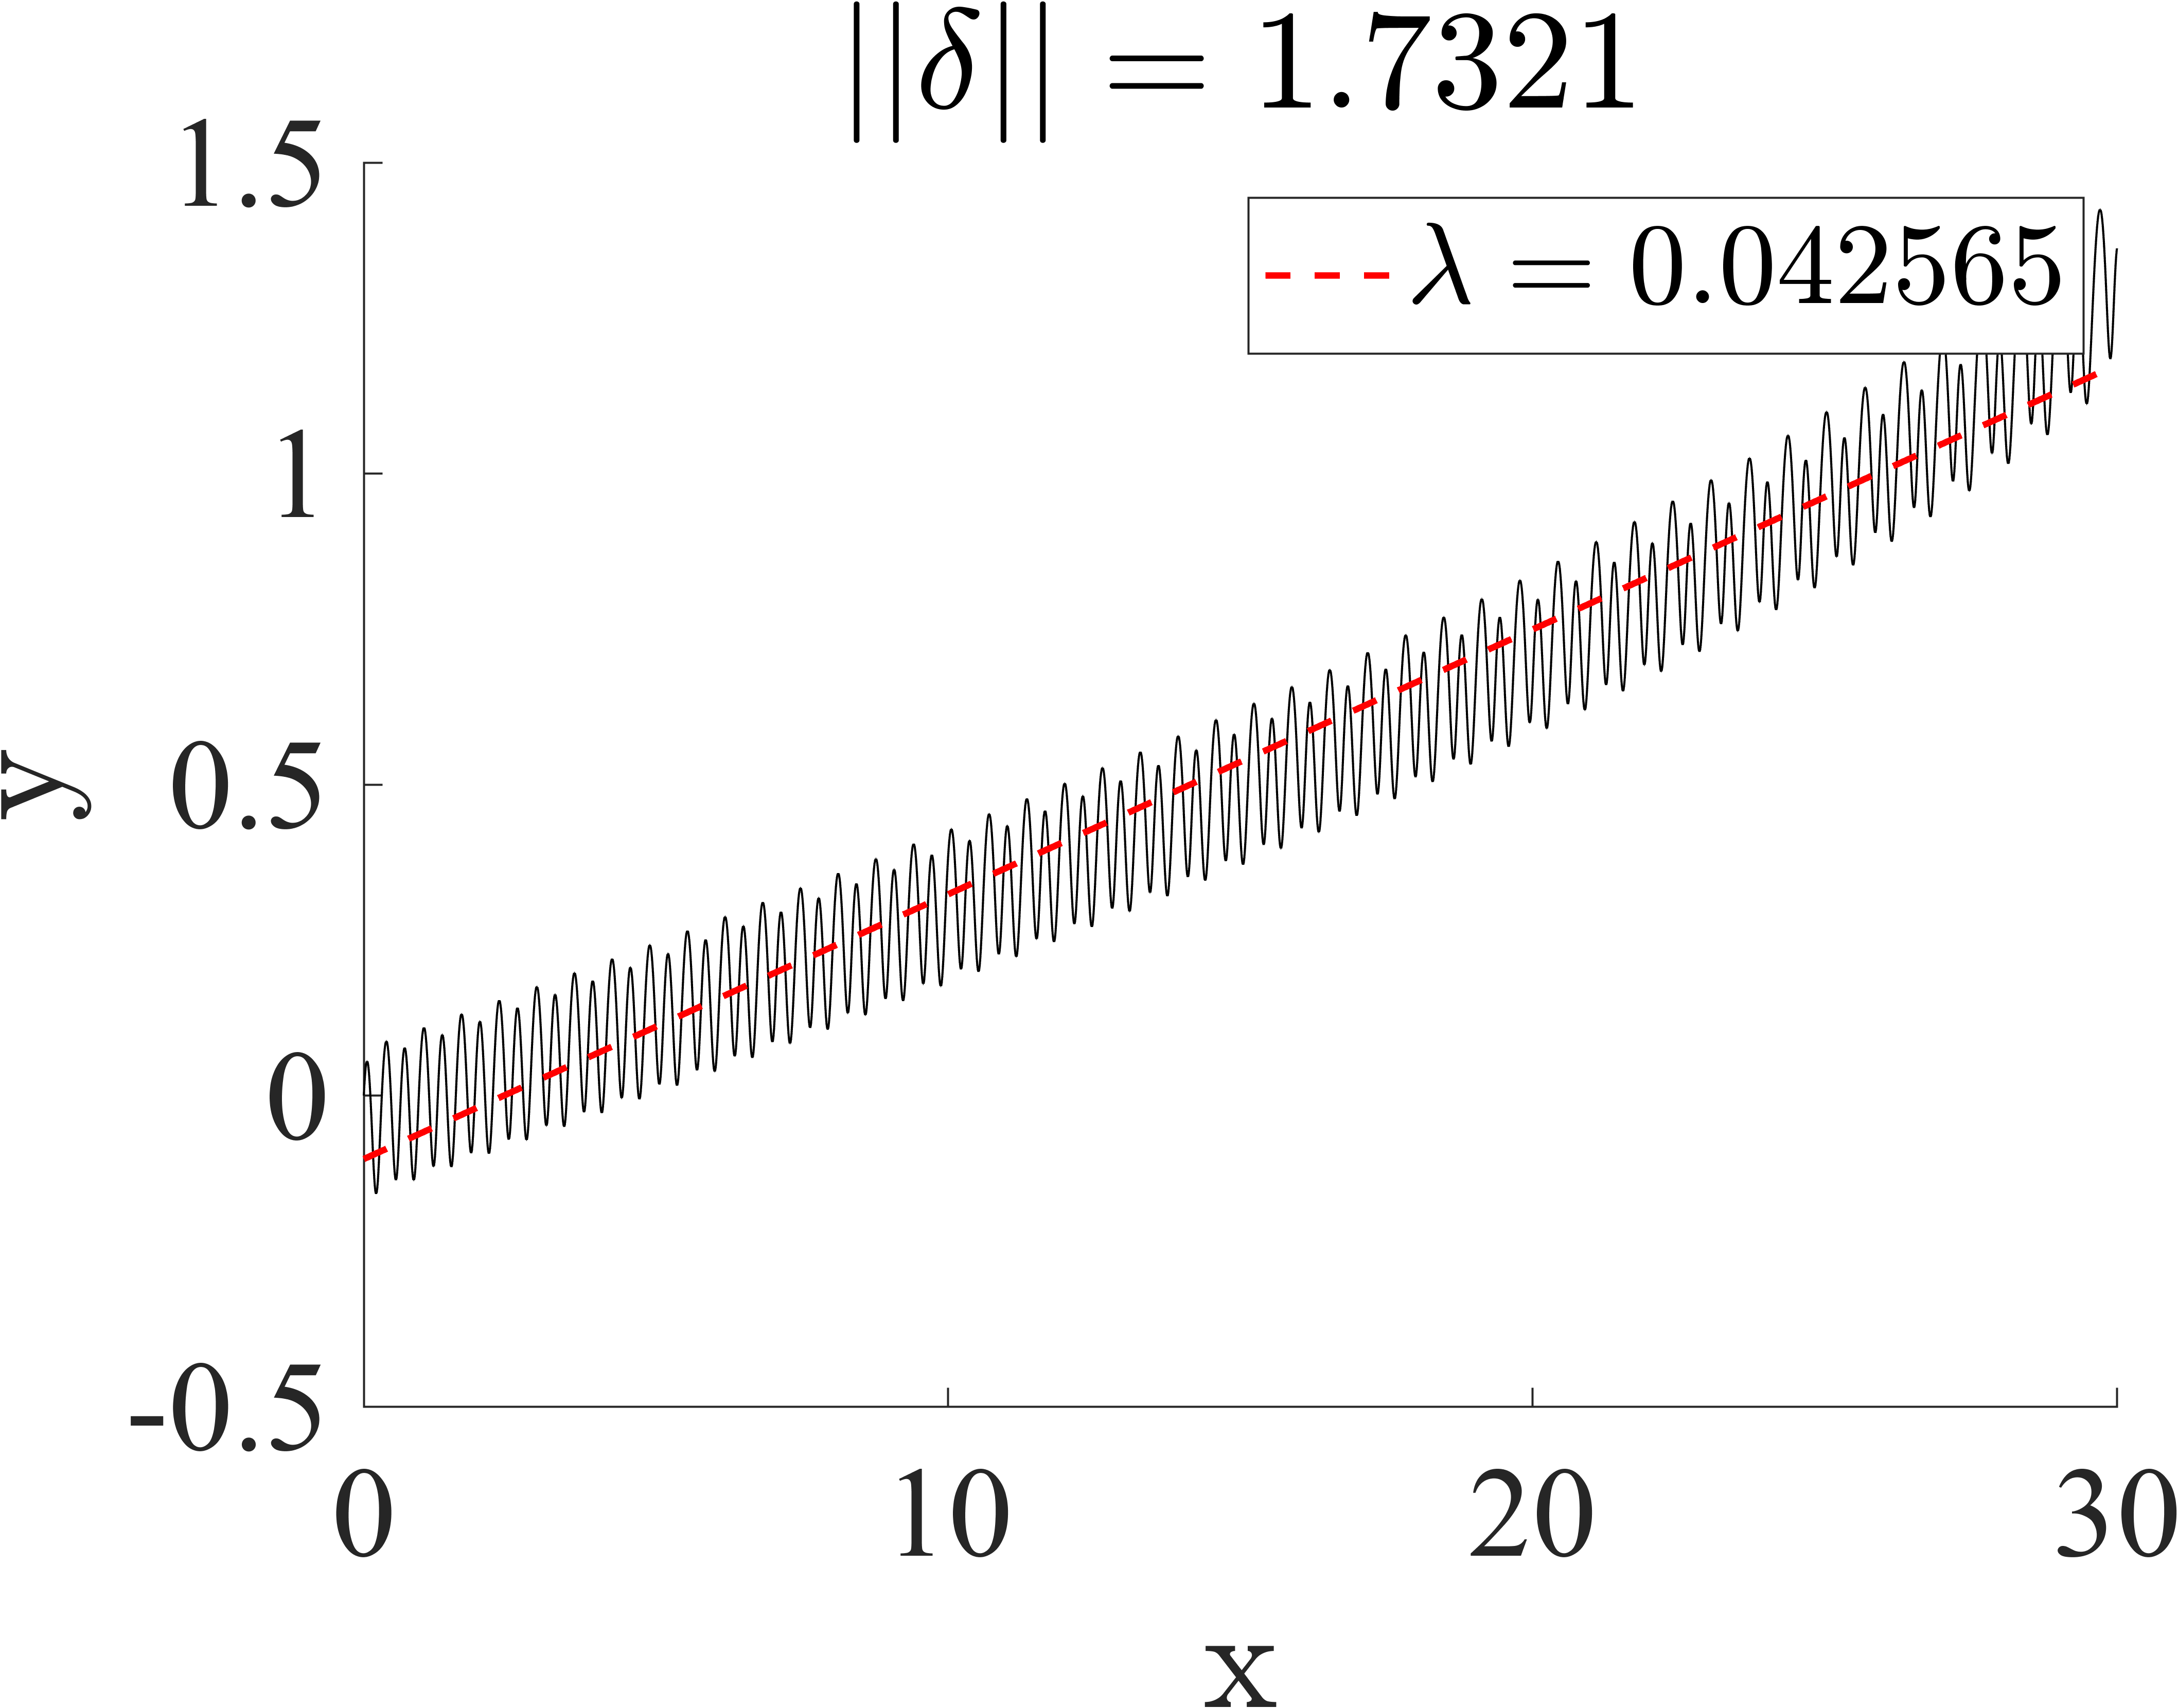
\includegraphics[width=8cm]{Lorenz_r25.73682_trajectories_discp2_delta4.png}
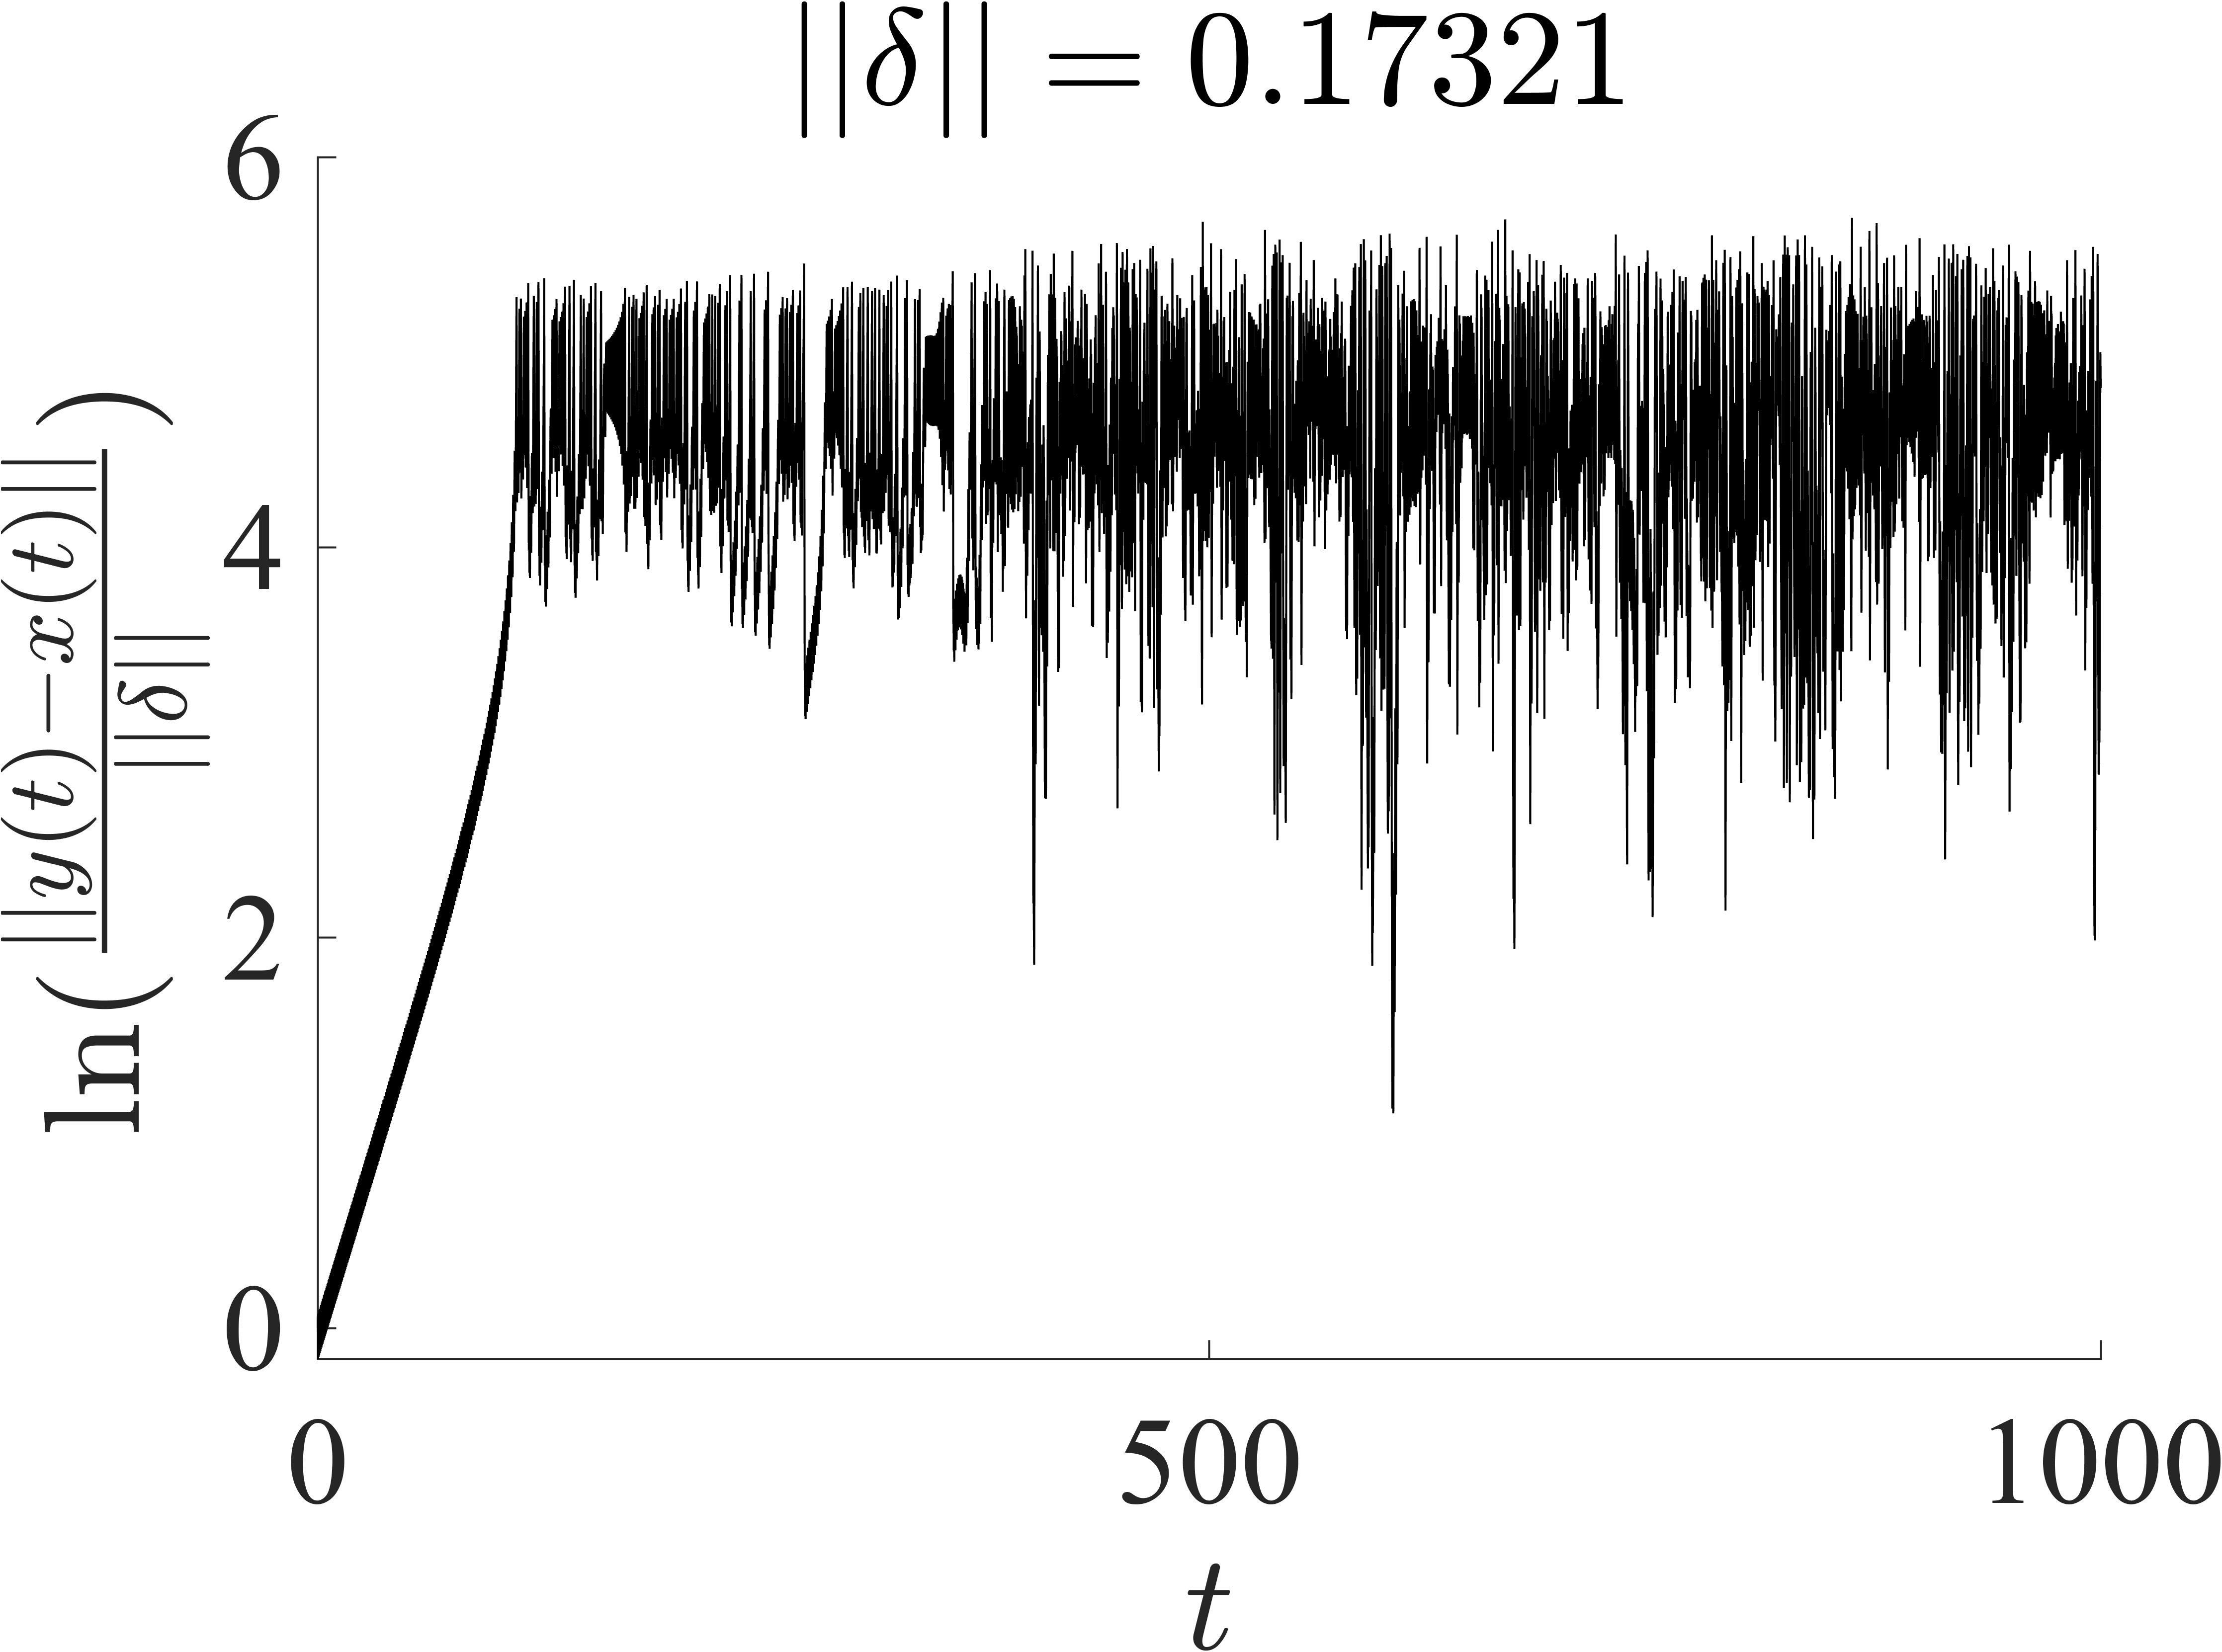
\includegraphics[width=8cm]{Lorenz_r25.73682_trajectories_discp.png}
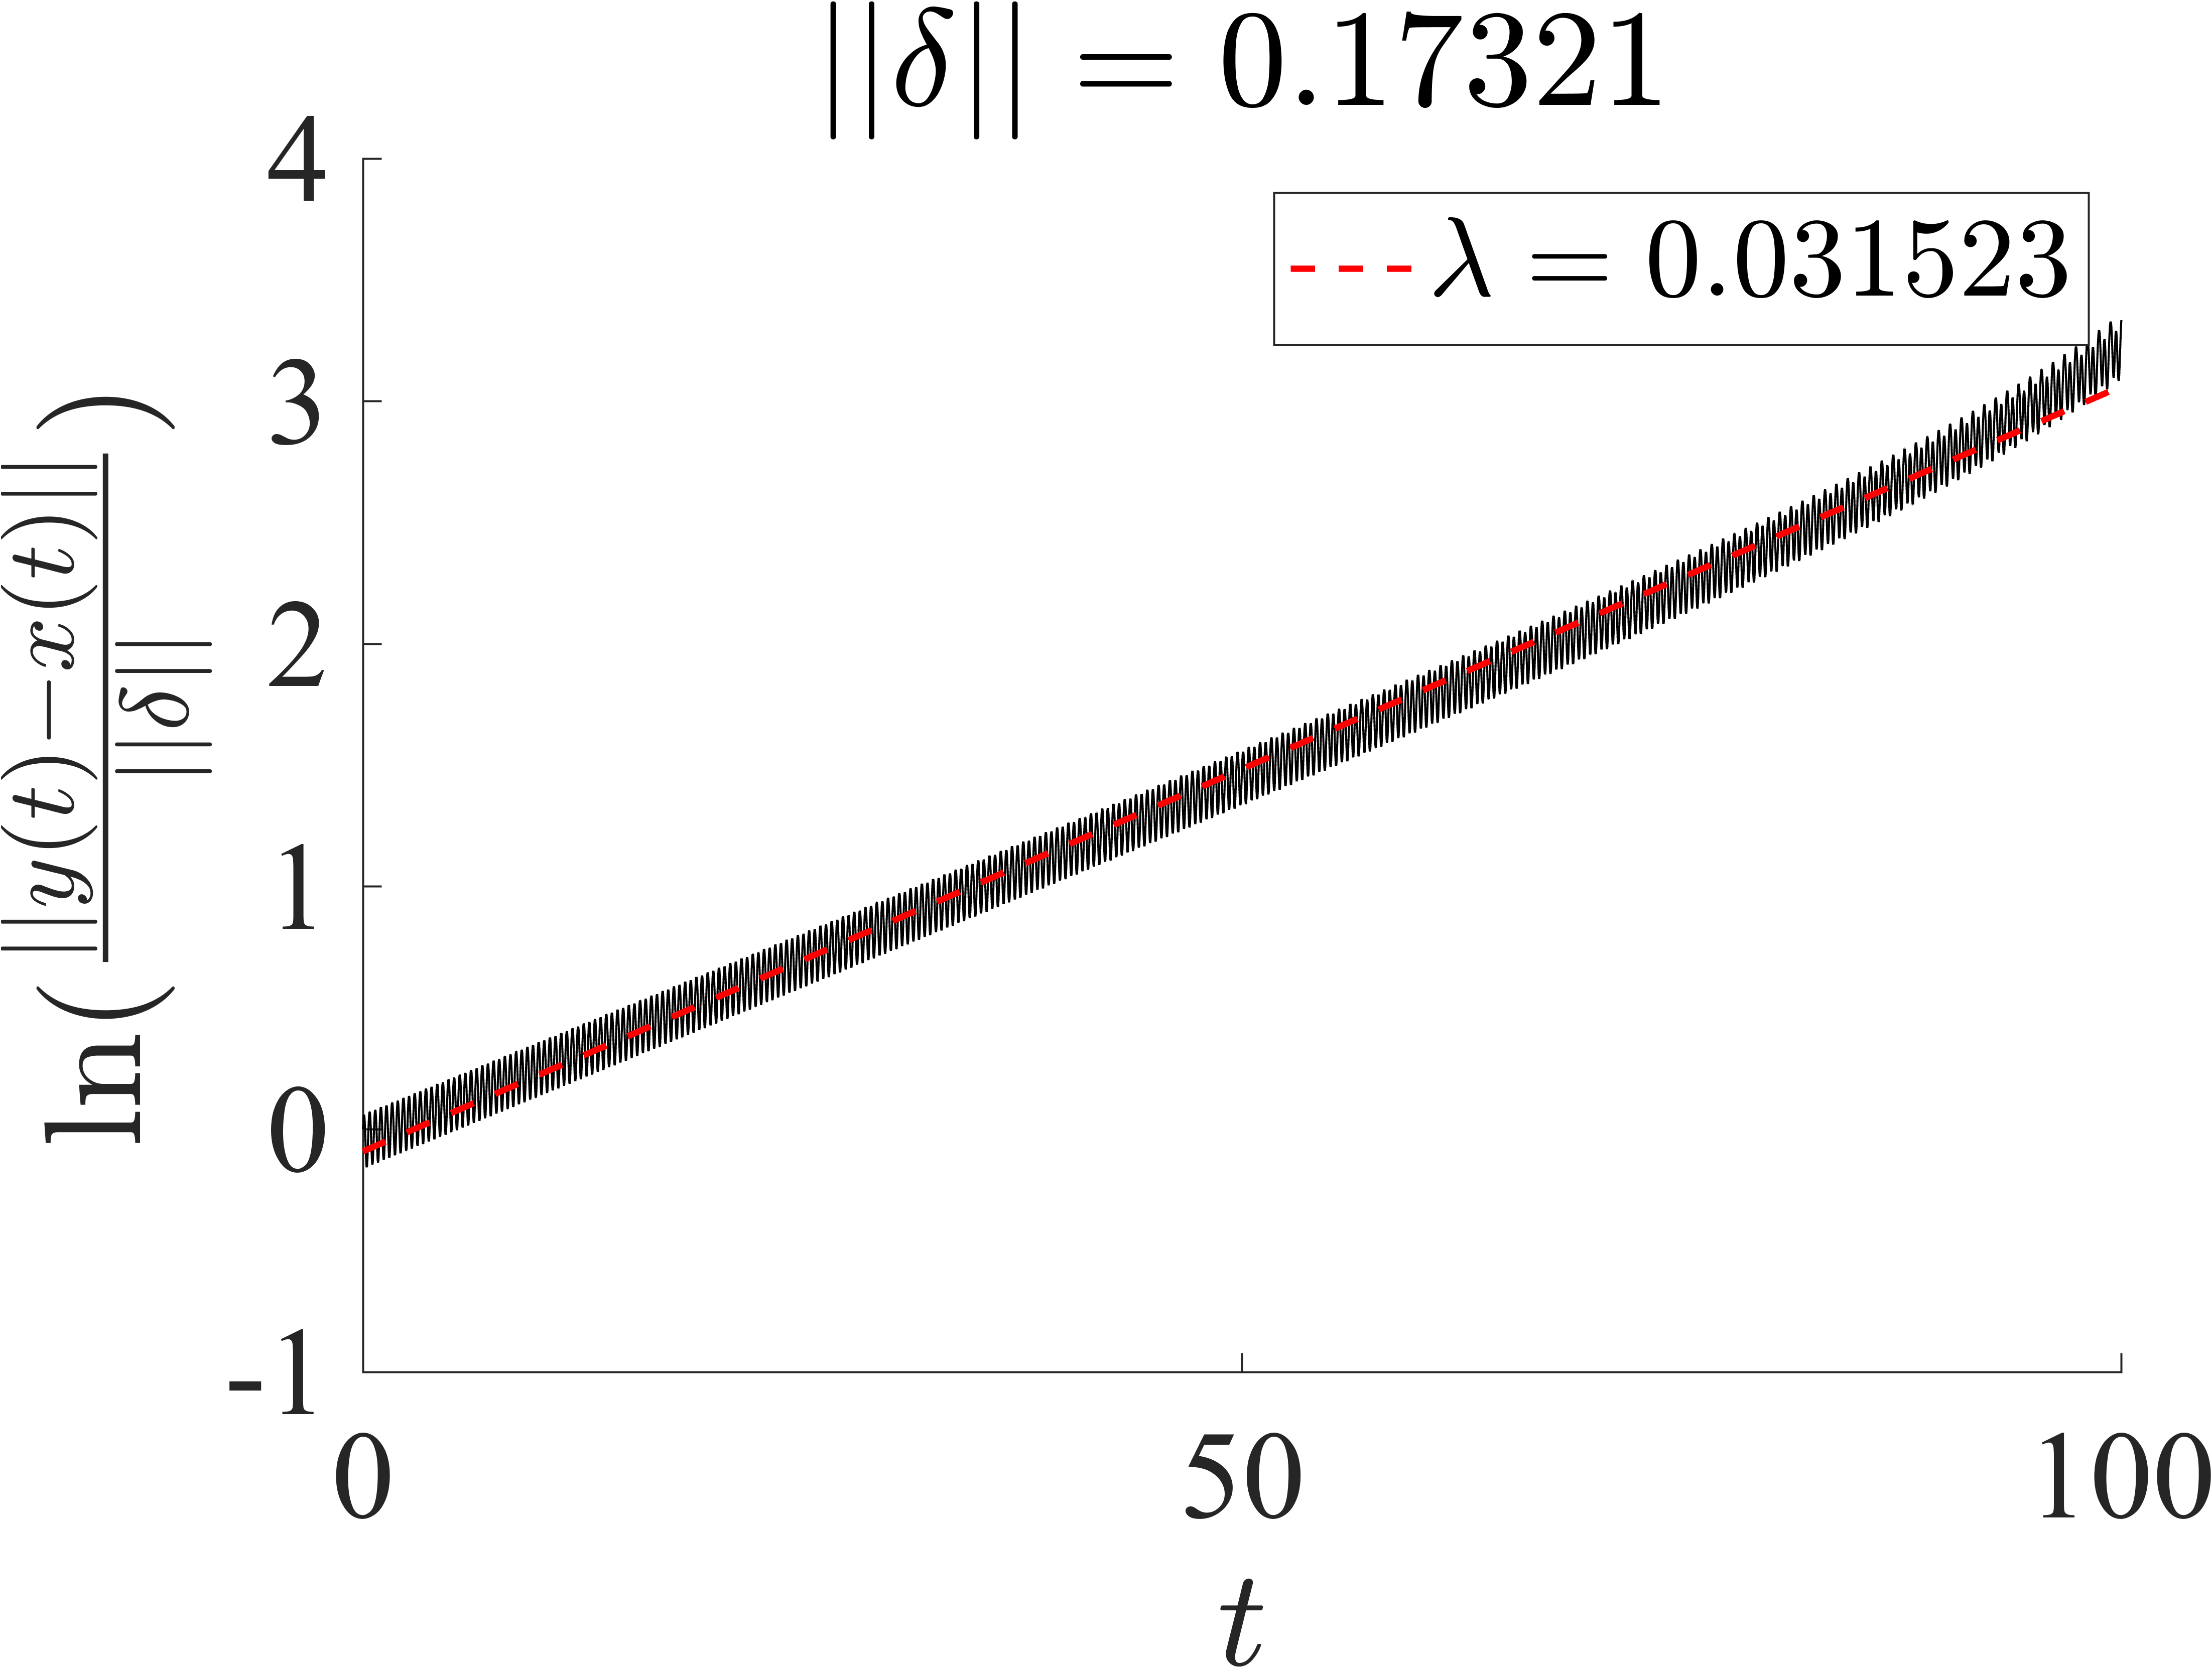
\includegraphics[width=8cm]{Lorenz_r25.73682_trajectories_discp2.png}
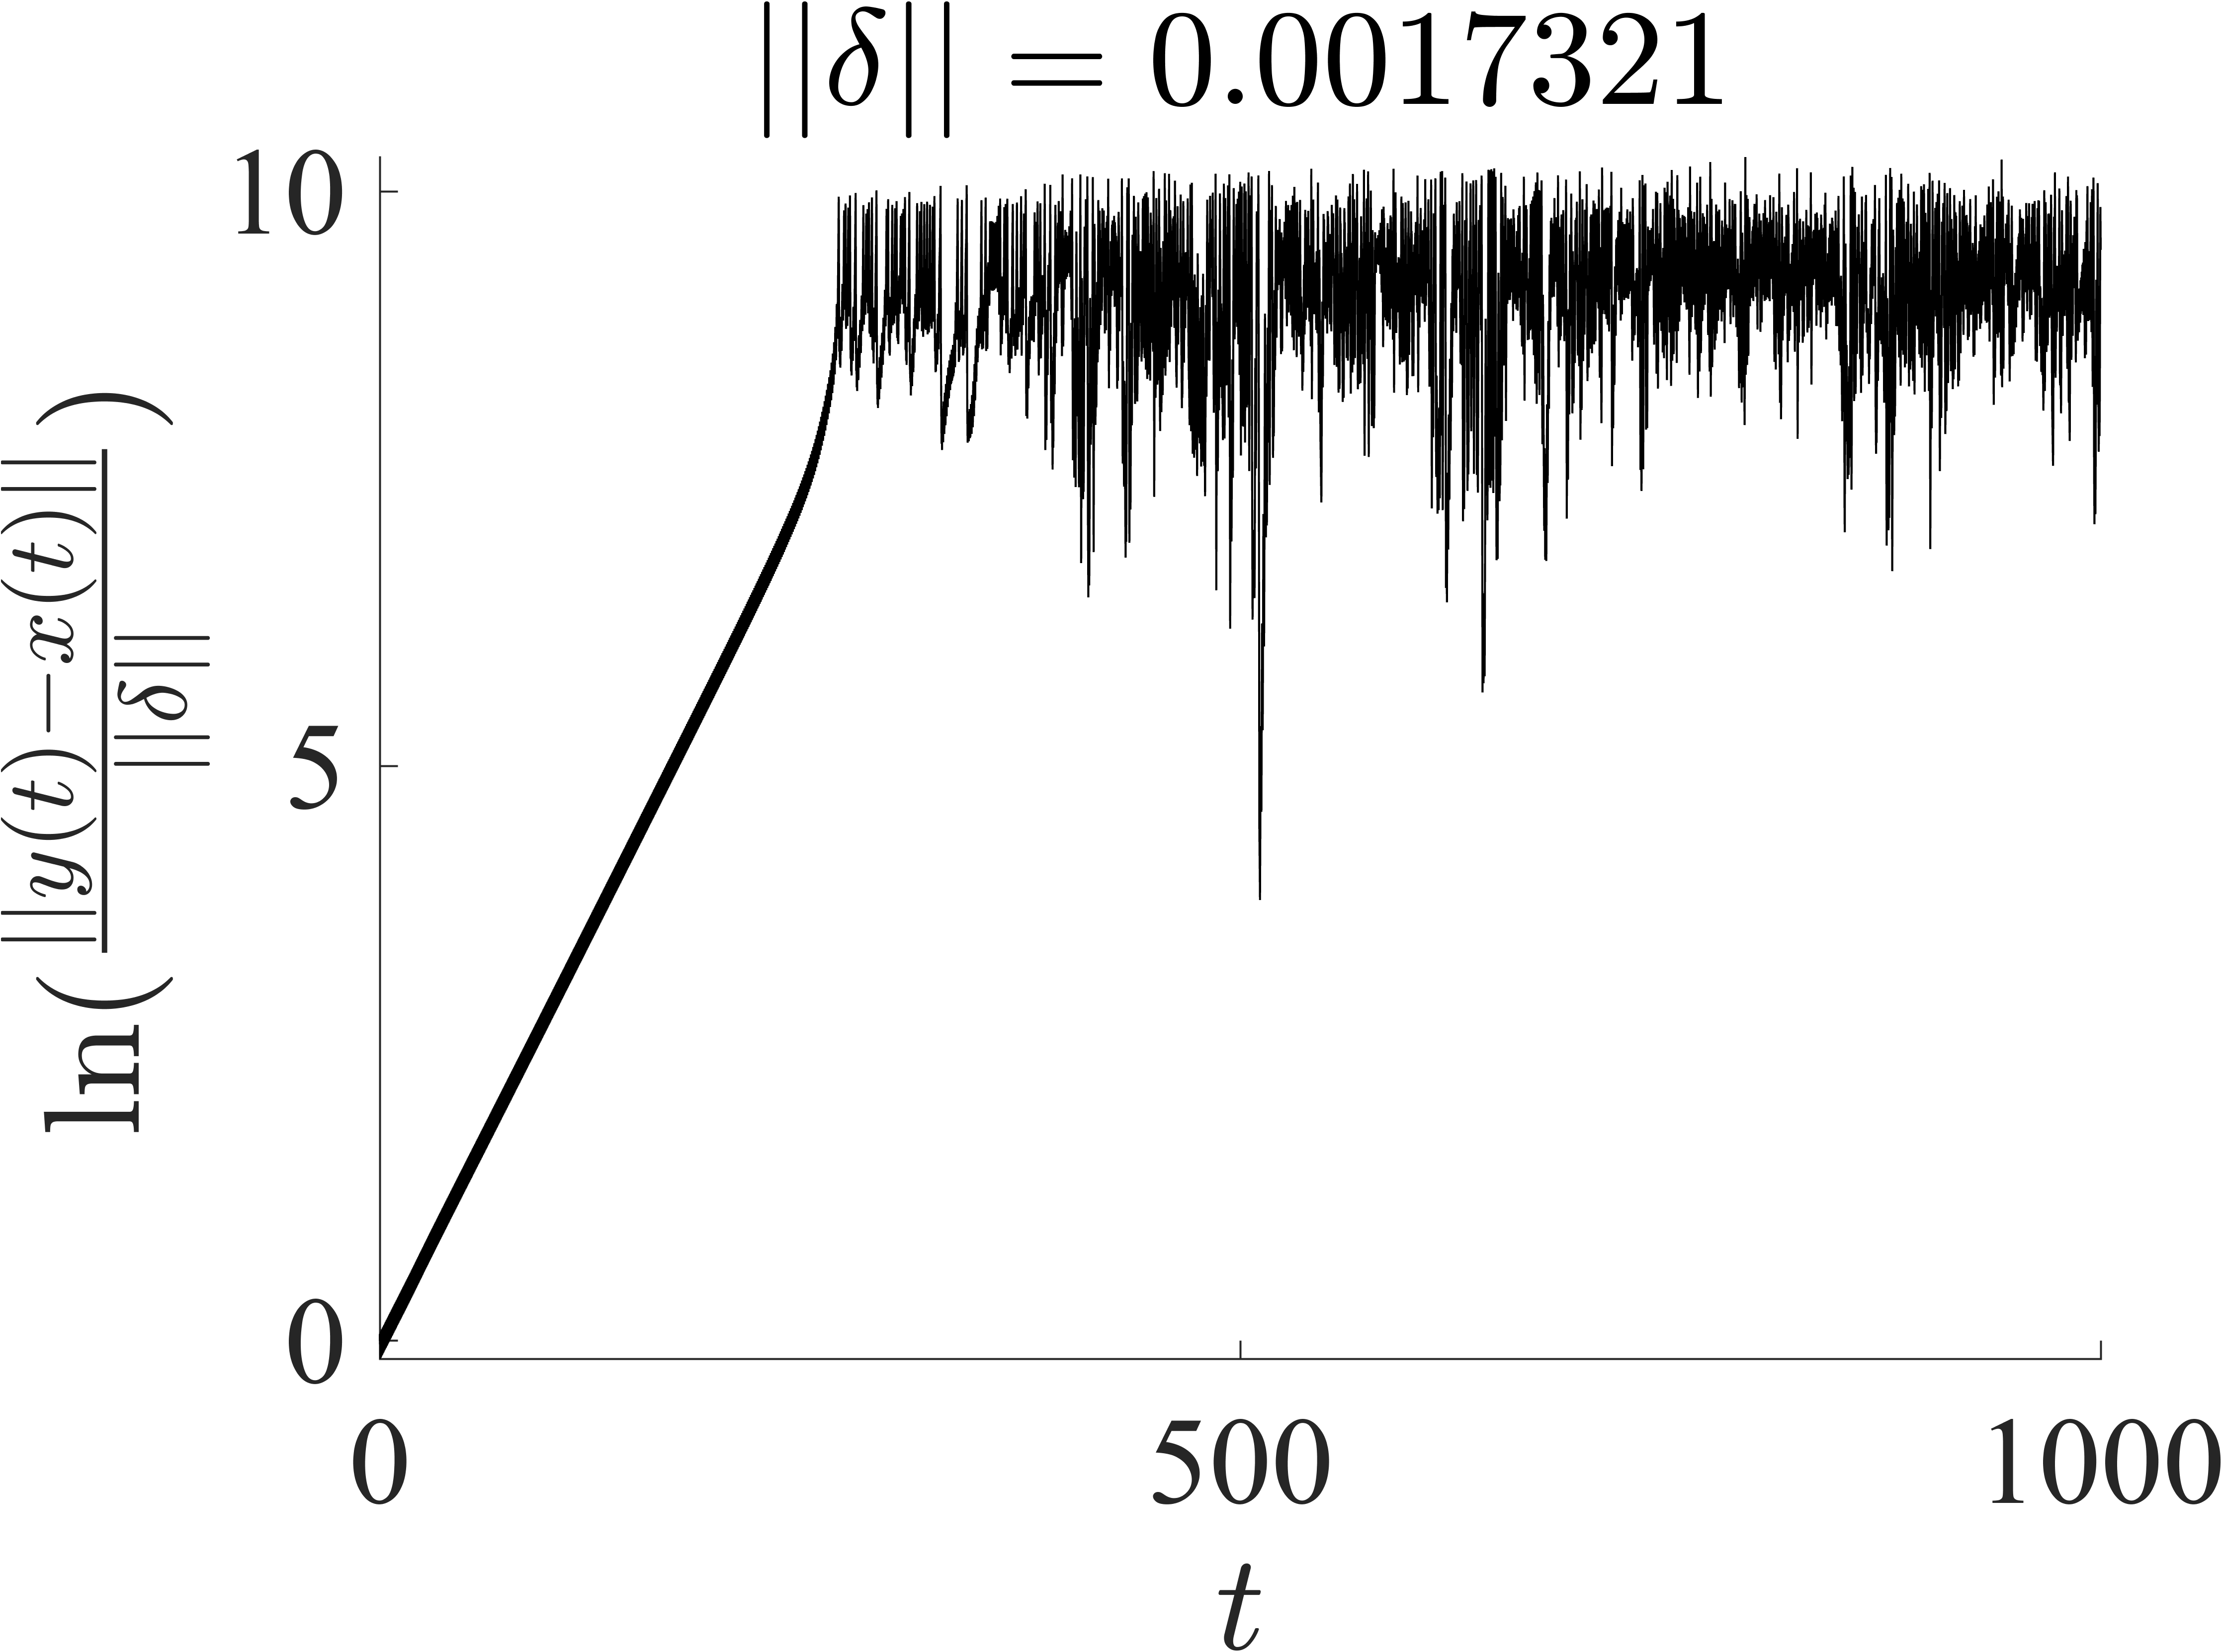
\includegraphics[width=8cm]{Lorenz_r25.73682_trajectories_discp_delta2.png}
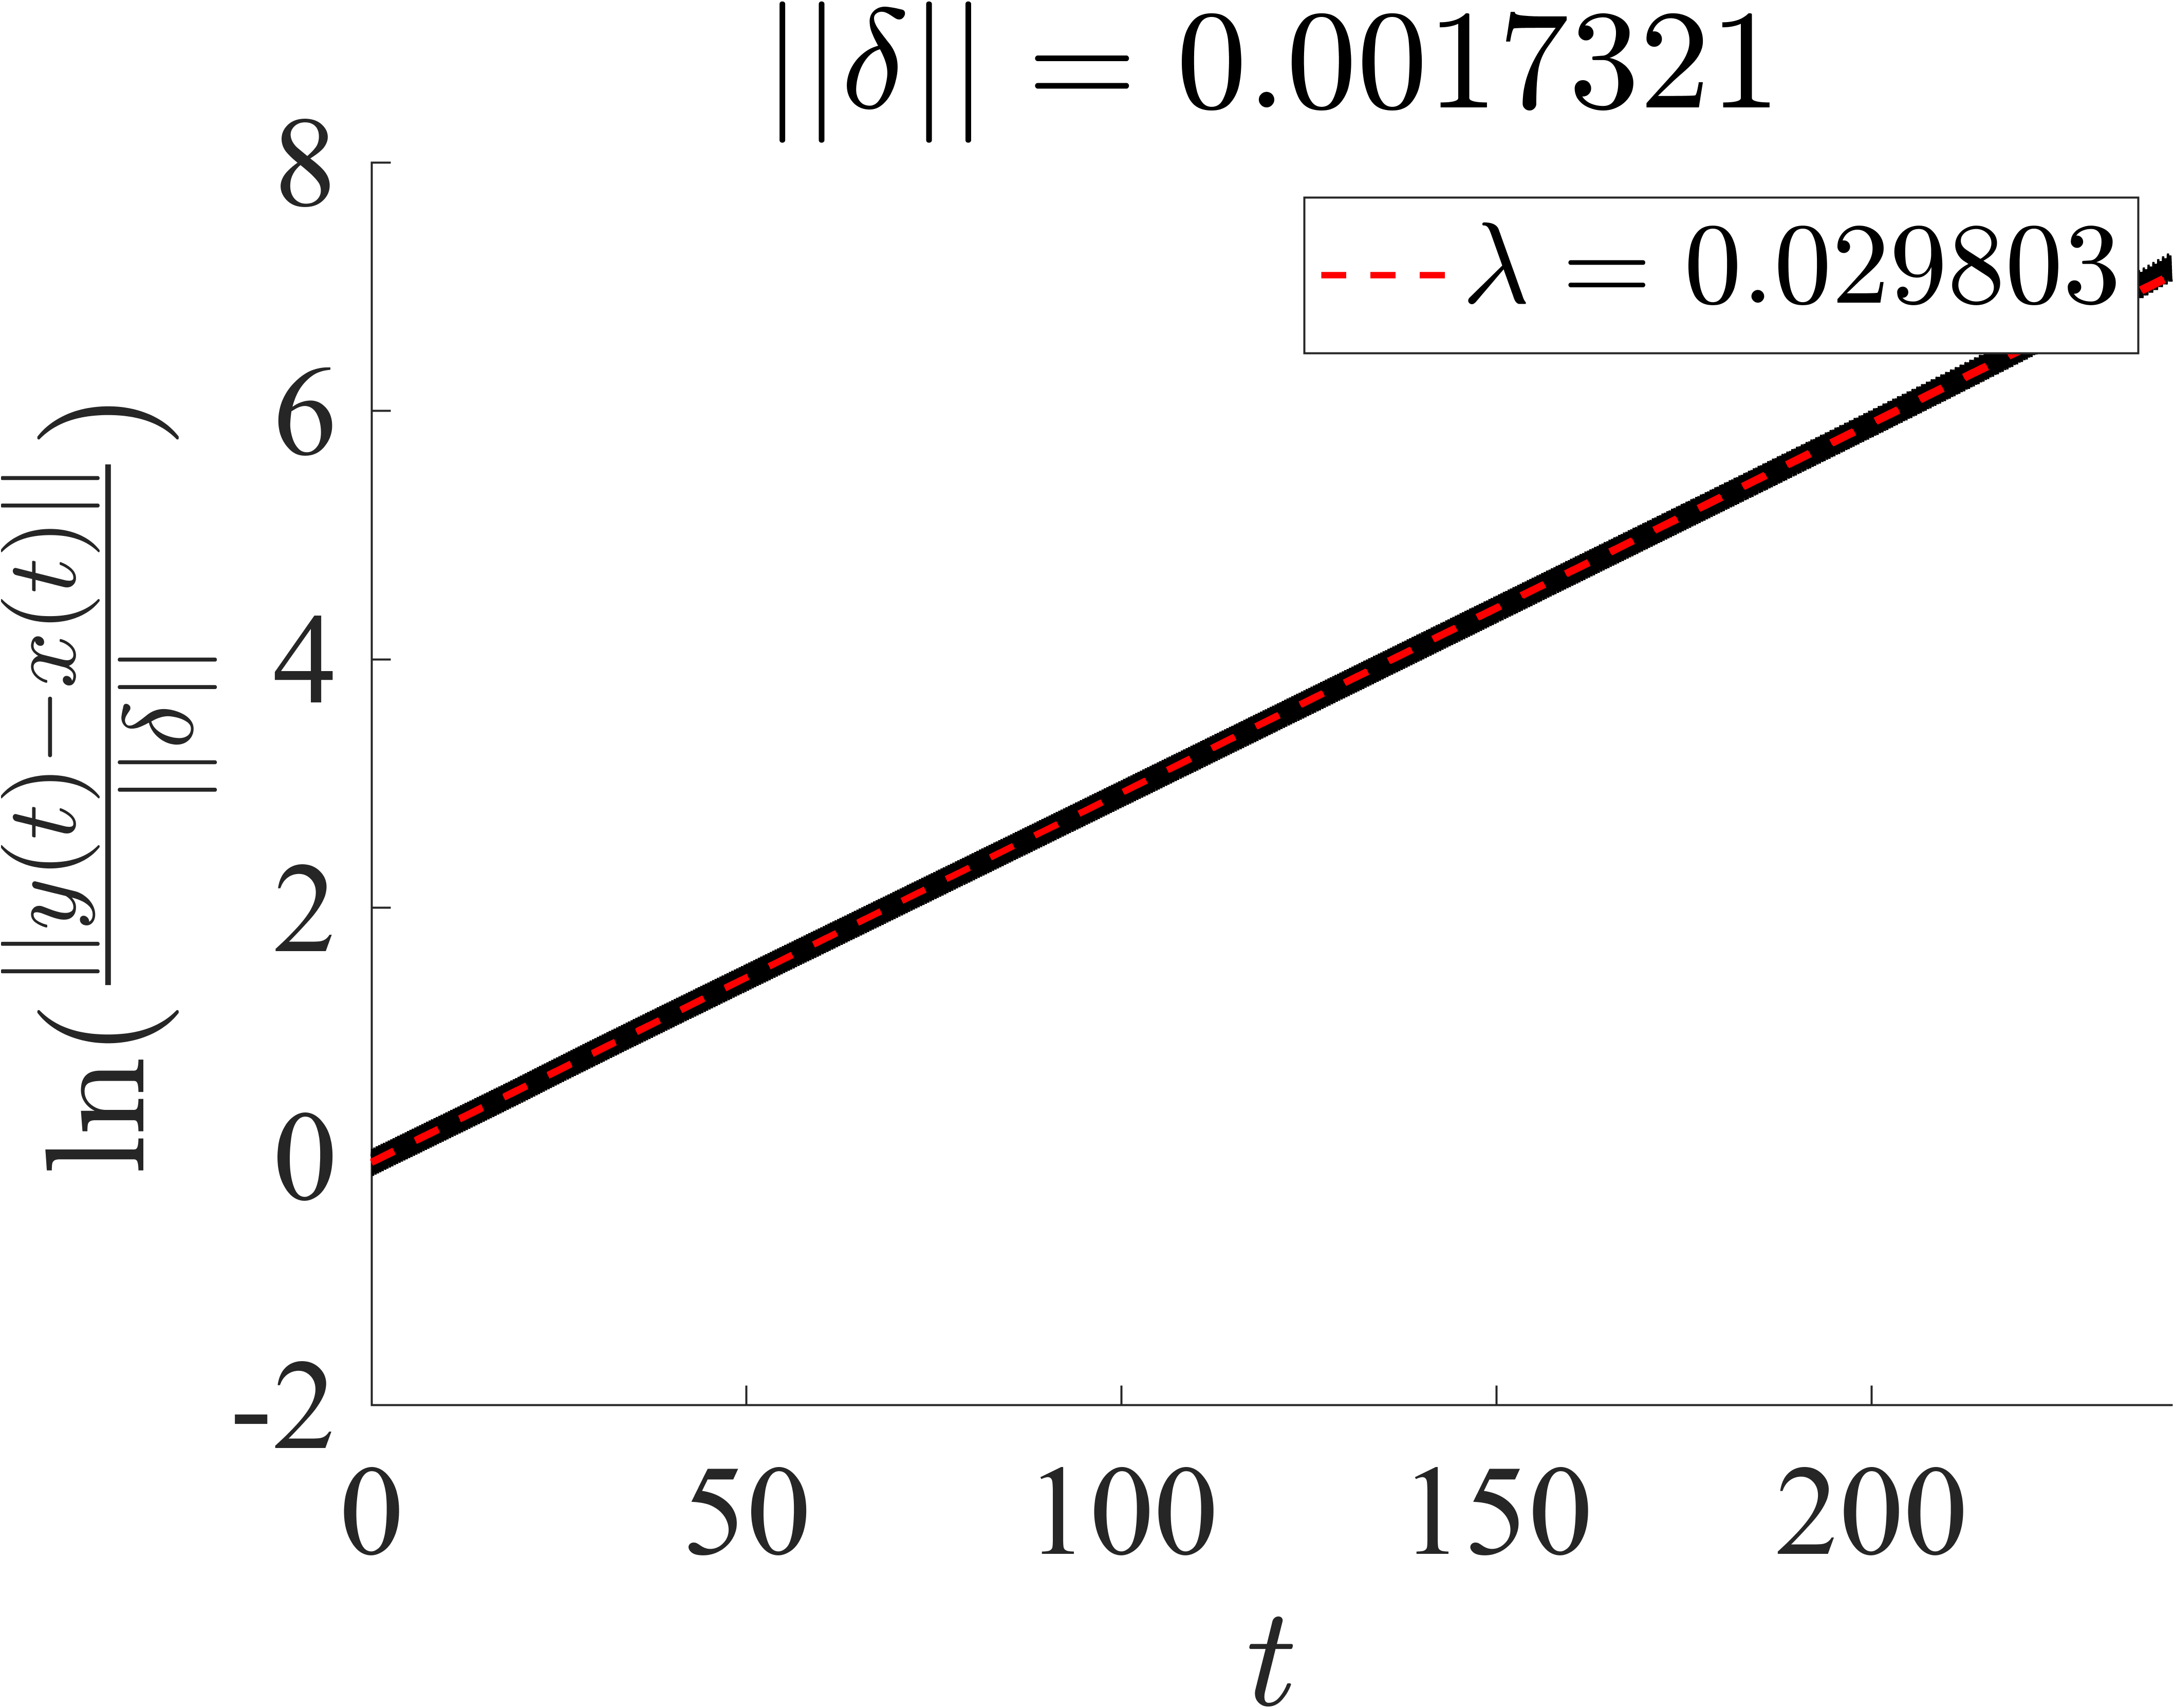
\includegraphics[width=8cm]{Lorenz_r25.73682_trajectories_discp2_delta2.png}
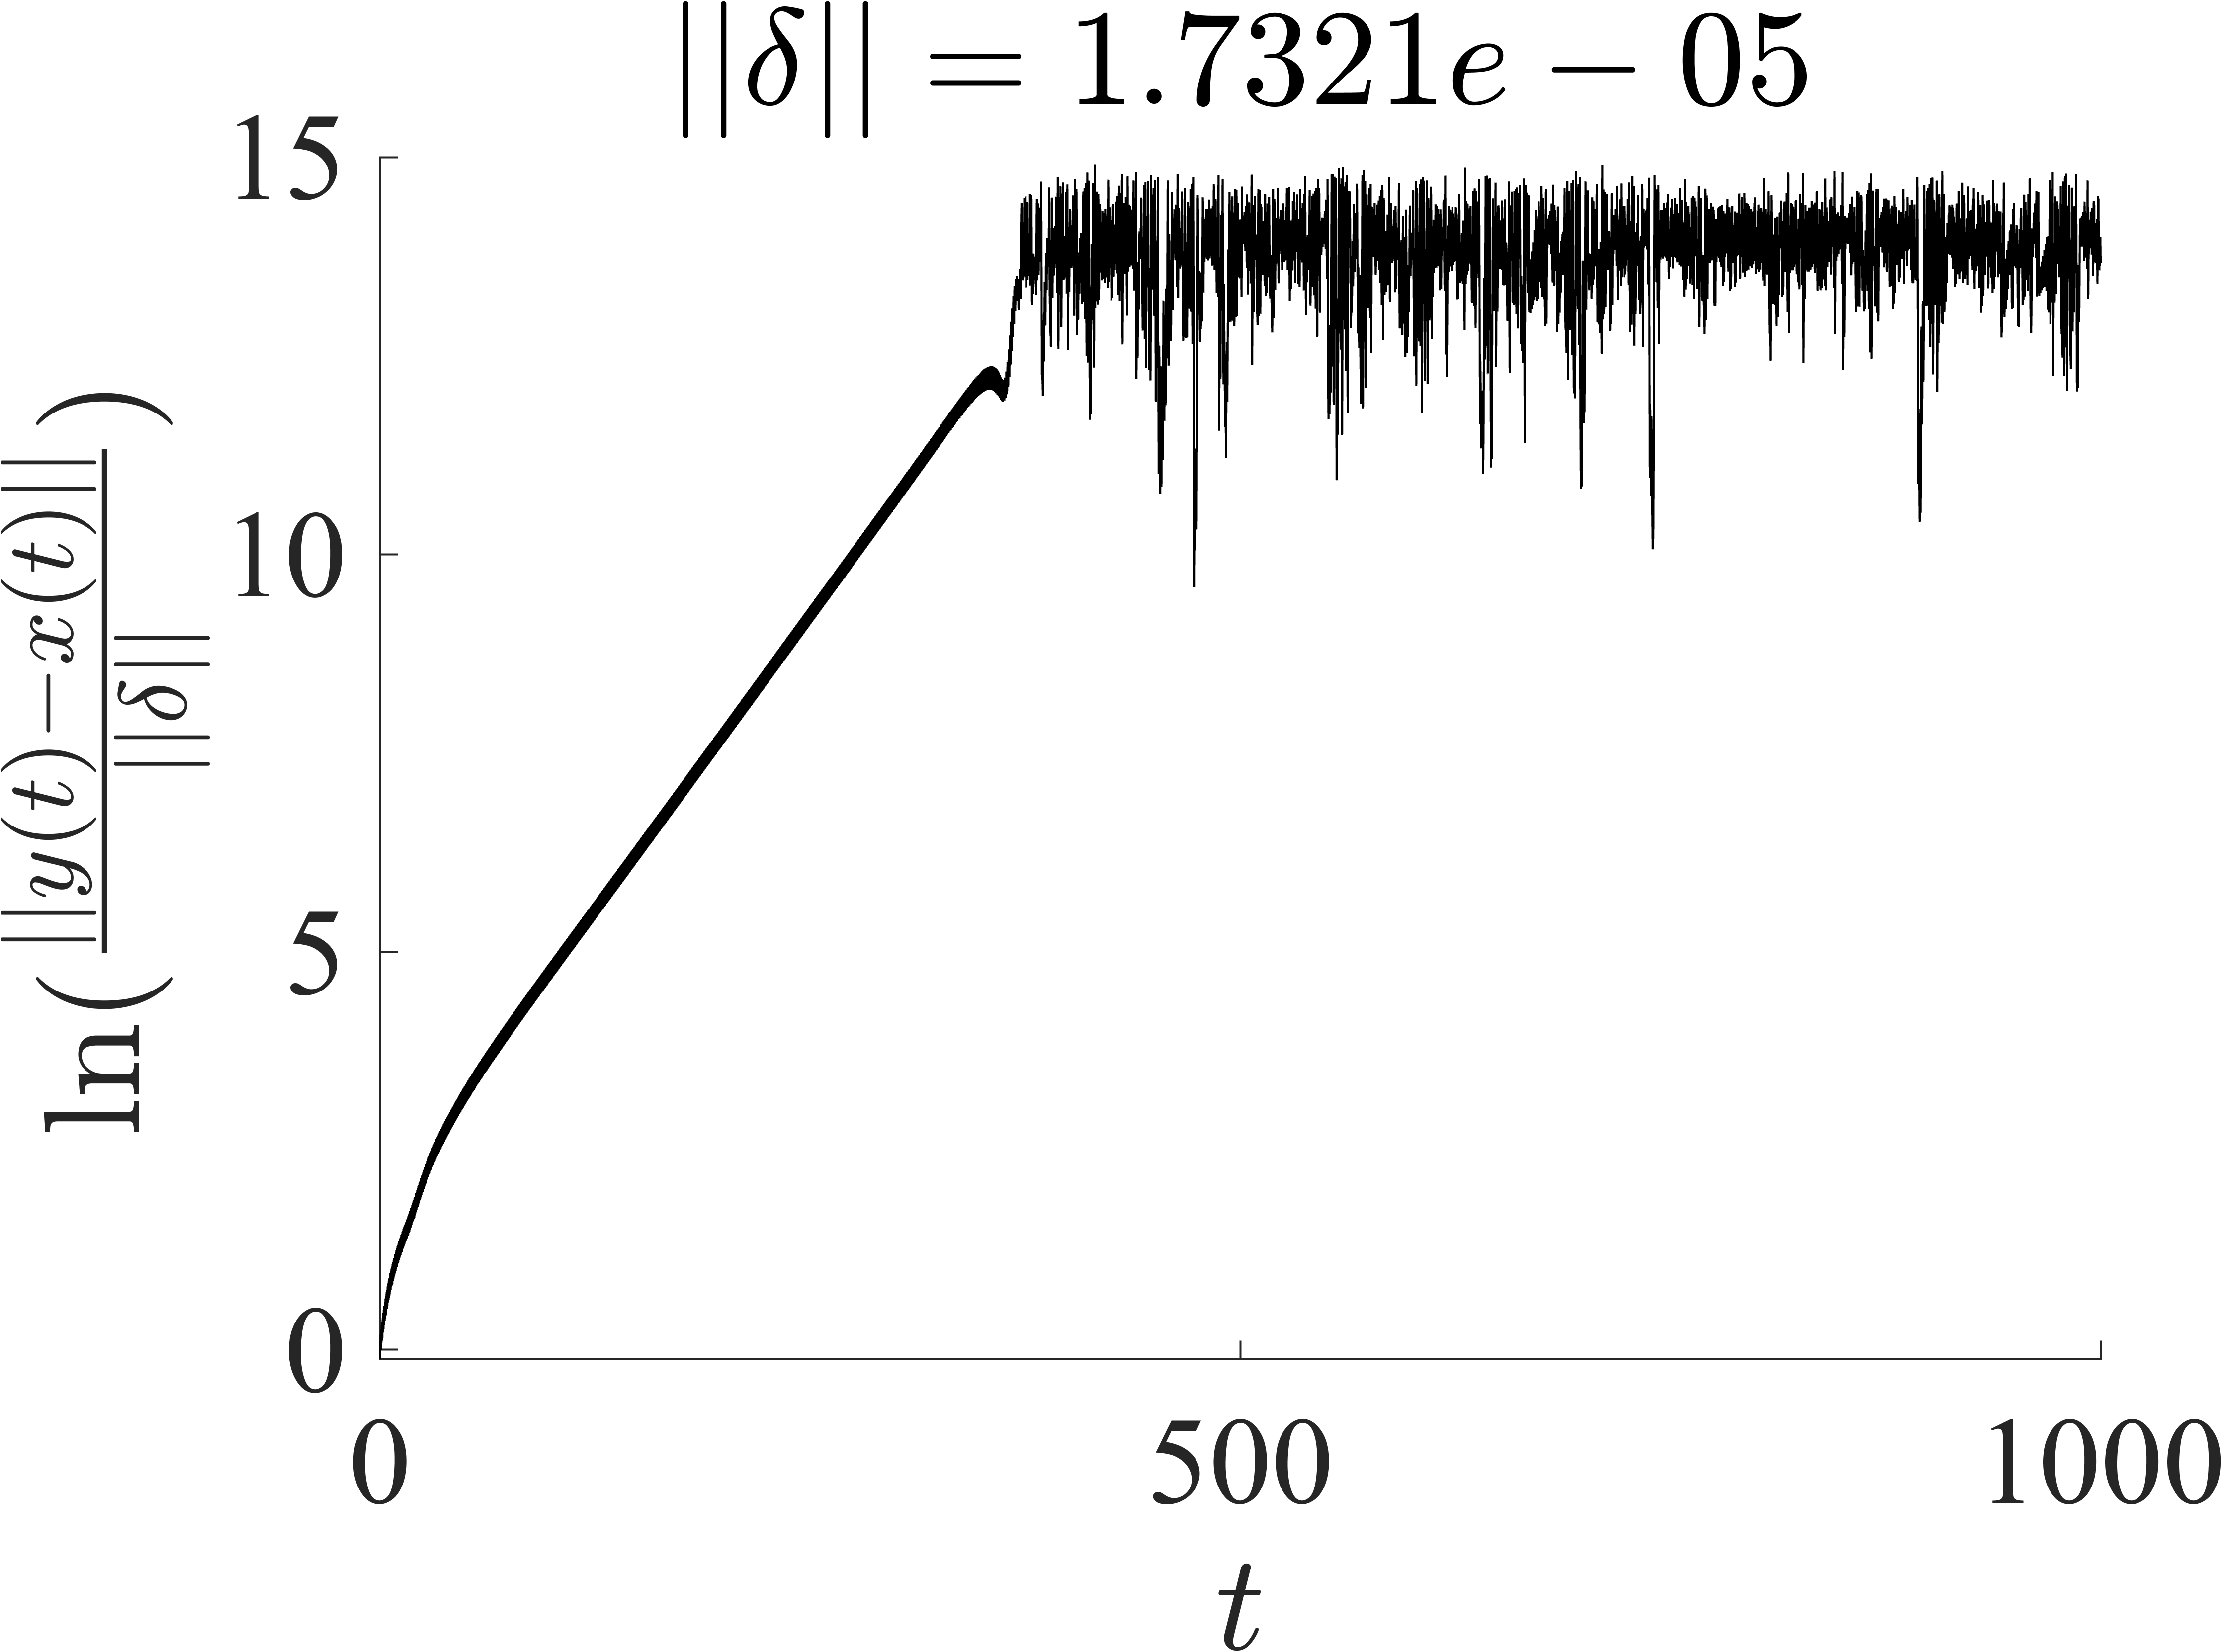
\includegraphics[width=8cm]{Lorenz_r25.73682_trajectories_discp_delta3.png}
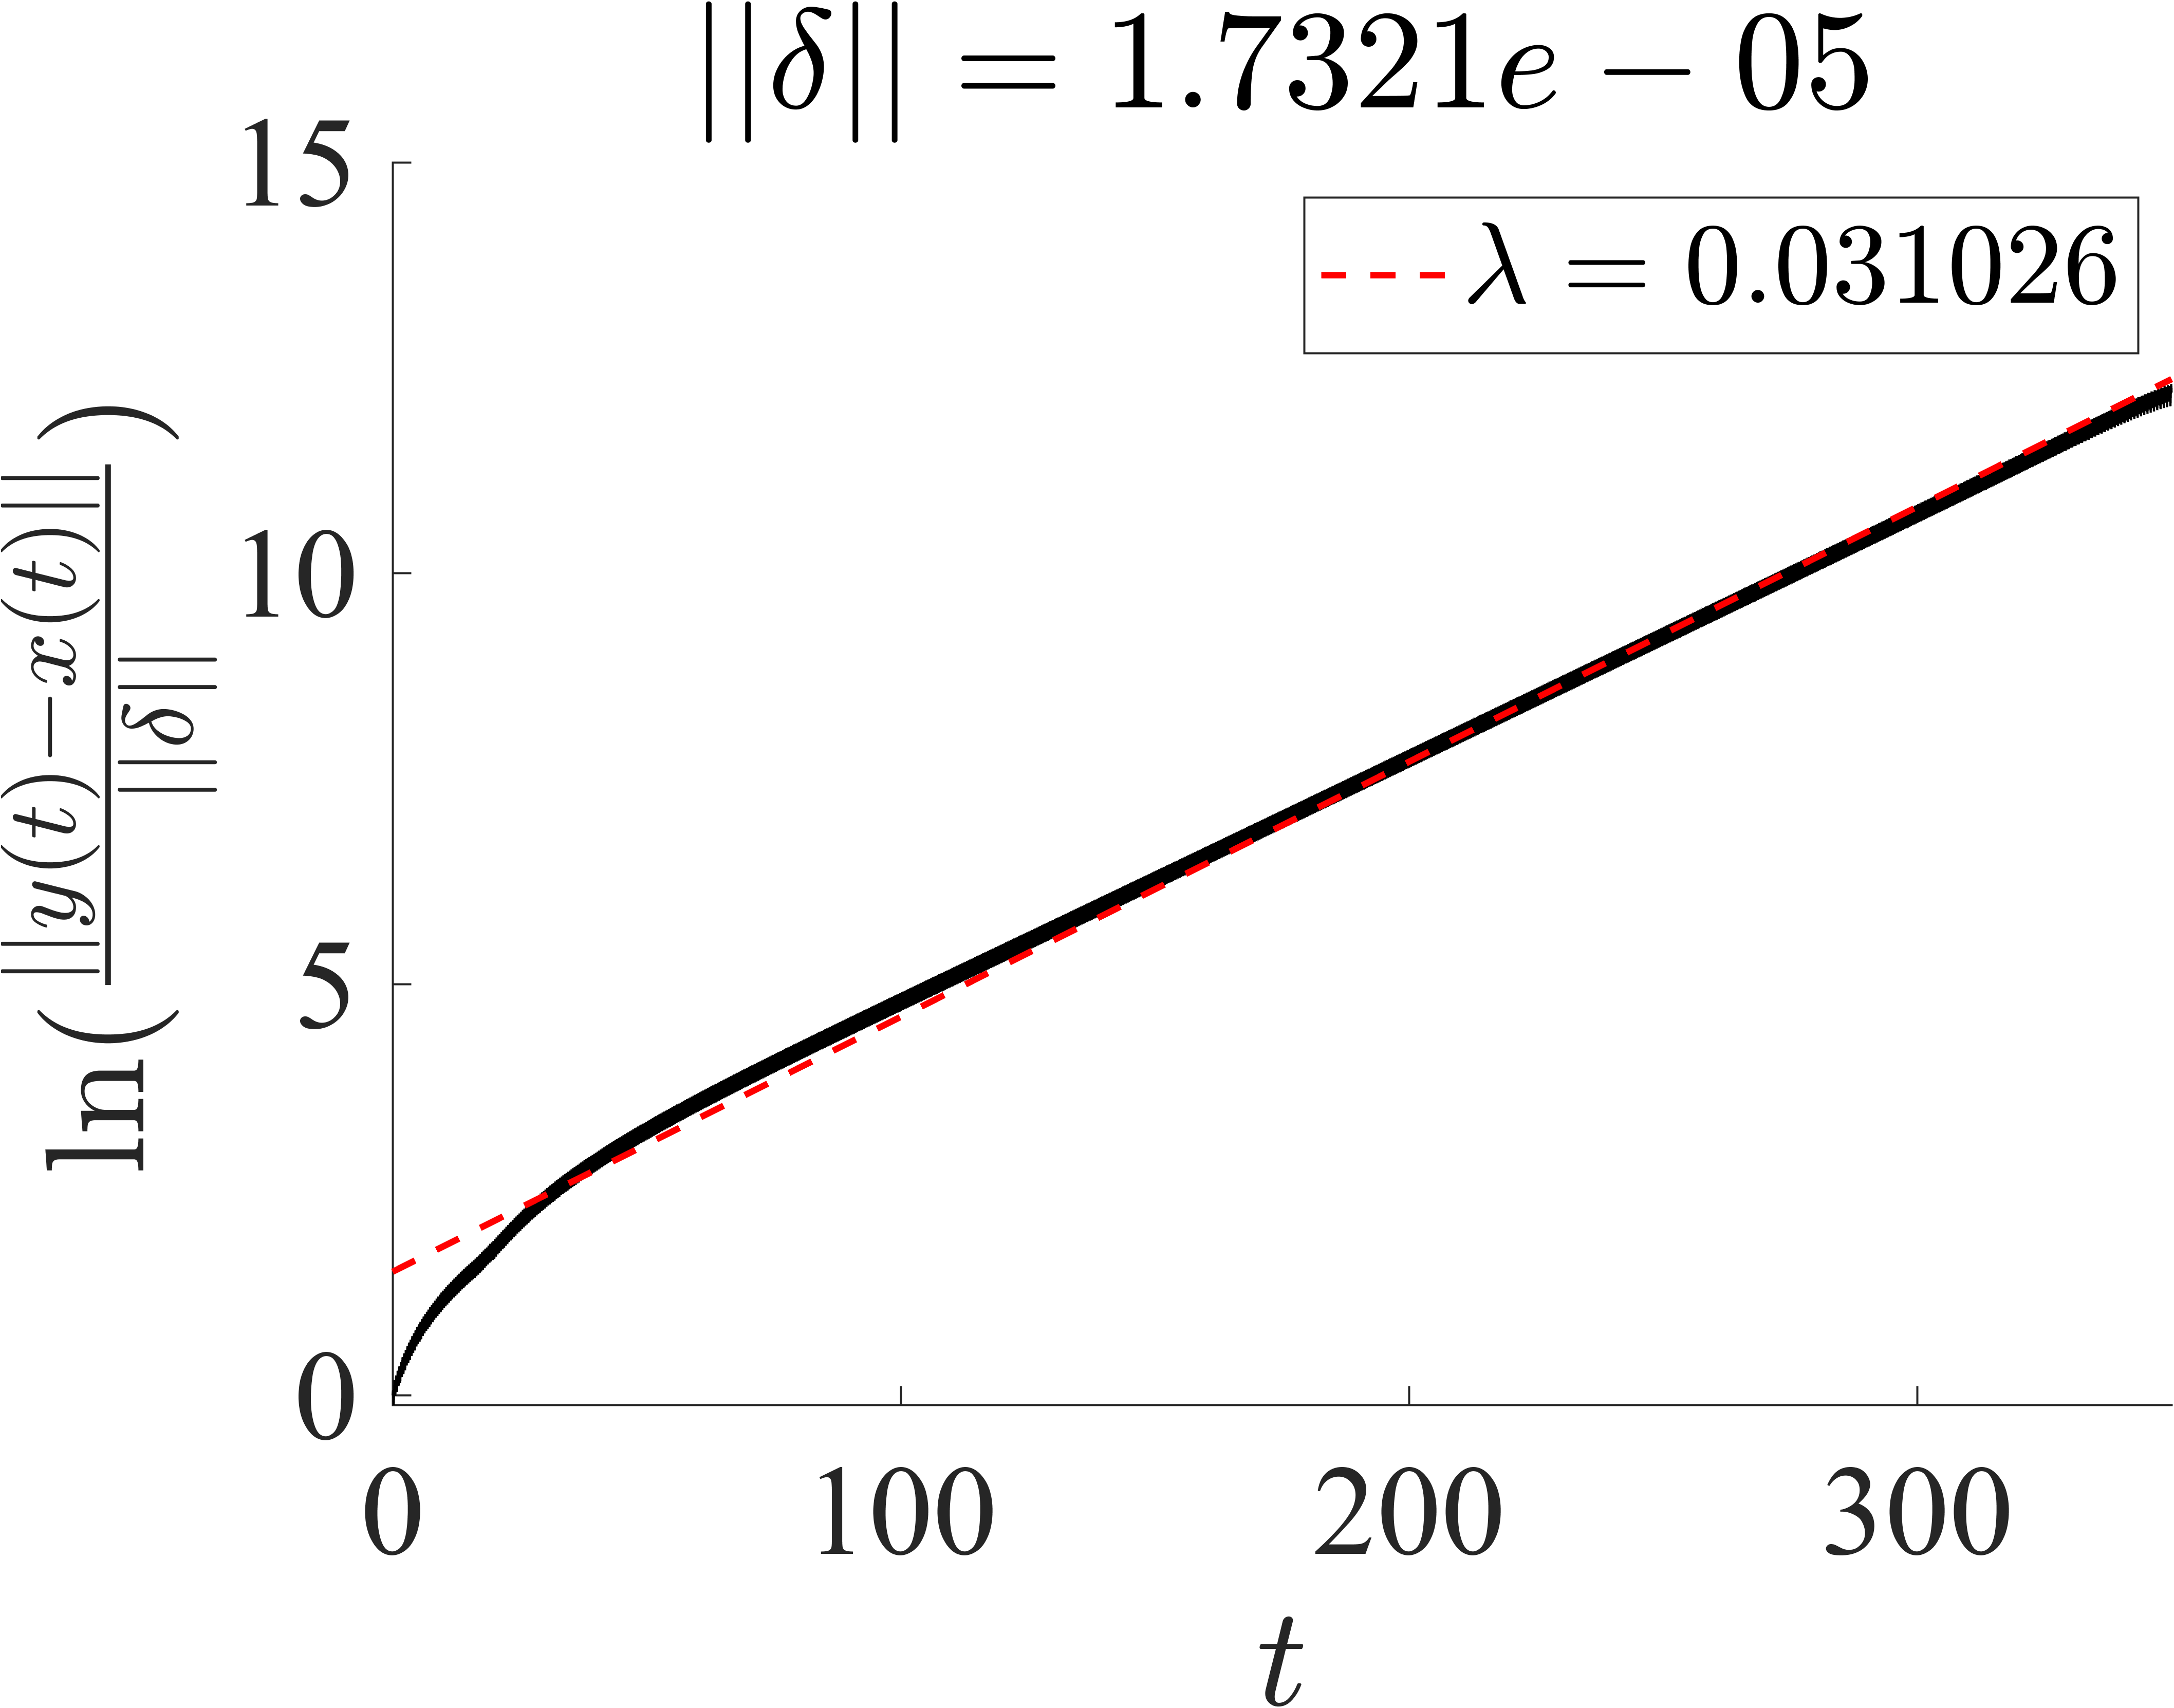
\includegraphics[width=8cm]{Lorenz_r25.73682_trajectories_discp2_delta3.png}
\caption{Lorenz Attractor: Two Trajectories}
\end{figure}

\clearpage

Now, I record the sequence of local maxima of the $z(t), \{z_1, z_2, ... \} $, and make a scatter plot of $z_{n+1}$ against $z_n$. This is the Lorenz Map, which we see below:
\begin{figure}[h]
\centering
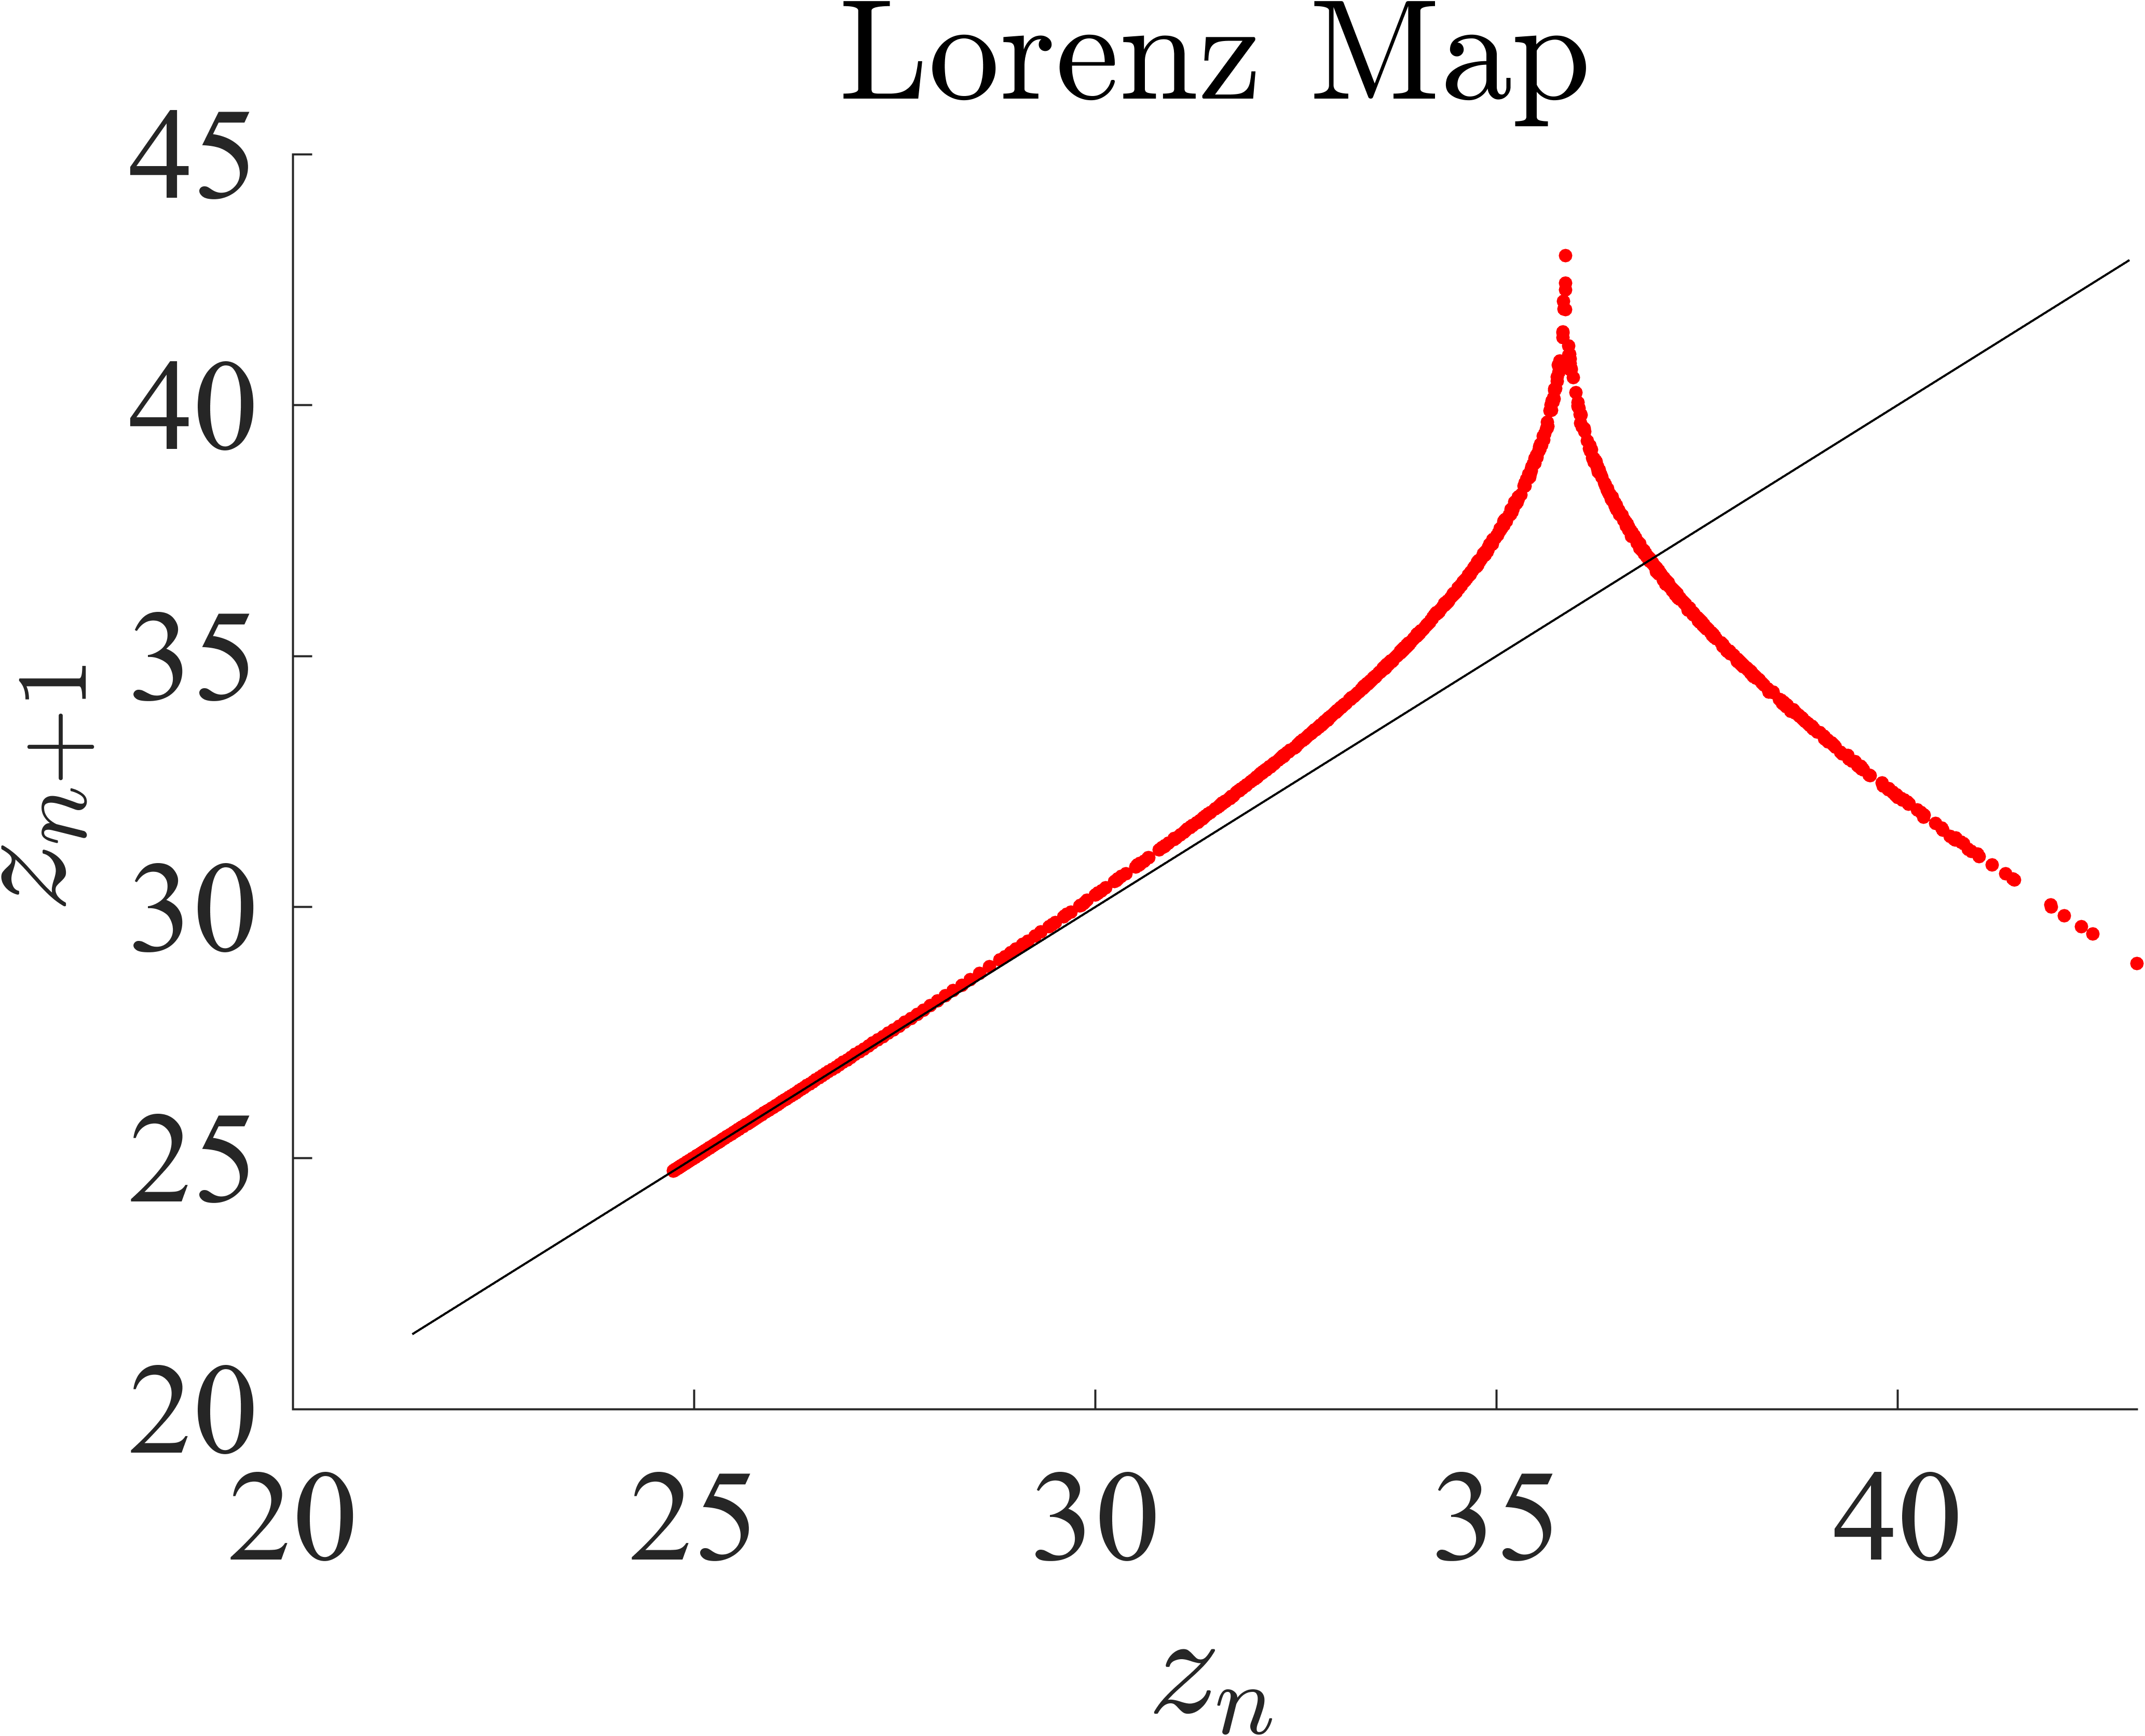
\includegraphics[width=8cm]{Lorenz_Map.png}
\caption{Lorenz Map}
\end{figure}

Here I plot some solutions to the Lorenz map using cobweb diagrams. I use a simple approximation of the curve in which I use the data value from the local maxima of $z(t)$ to tell me where $z_{n+1}$ is (no interpolation). I obtain the following cobweb diagrams for different initial conditions. In the figure after that, I plot these cobweb diagrams with a lower density (smaller number of steps). 
\begin{figure}[h]
\centering
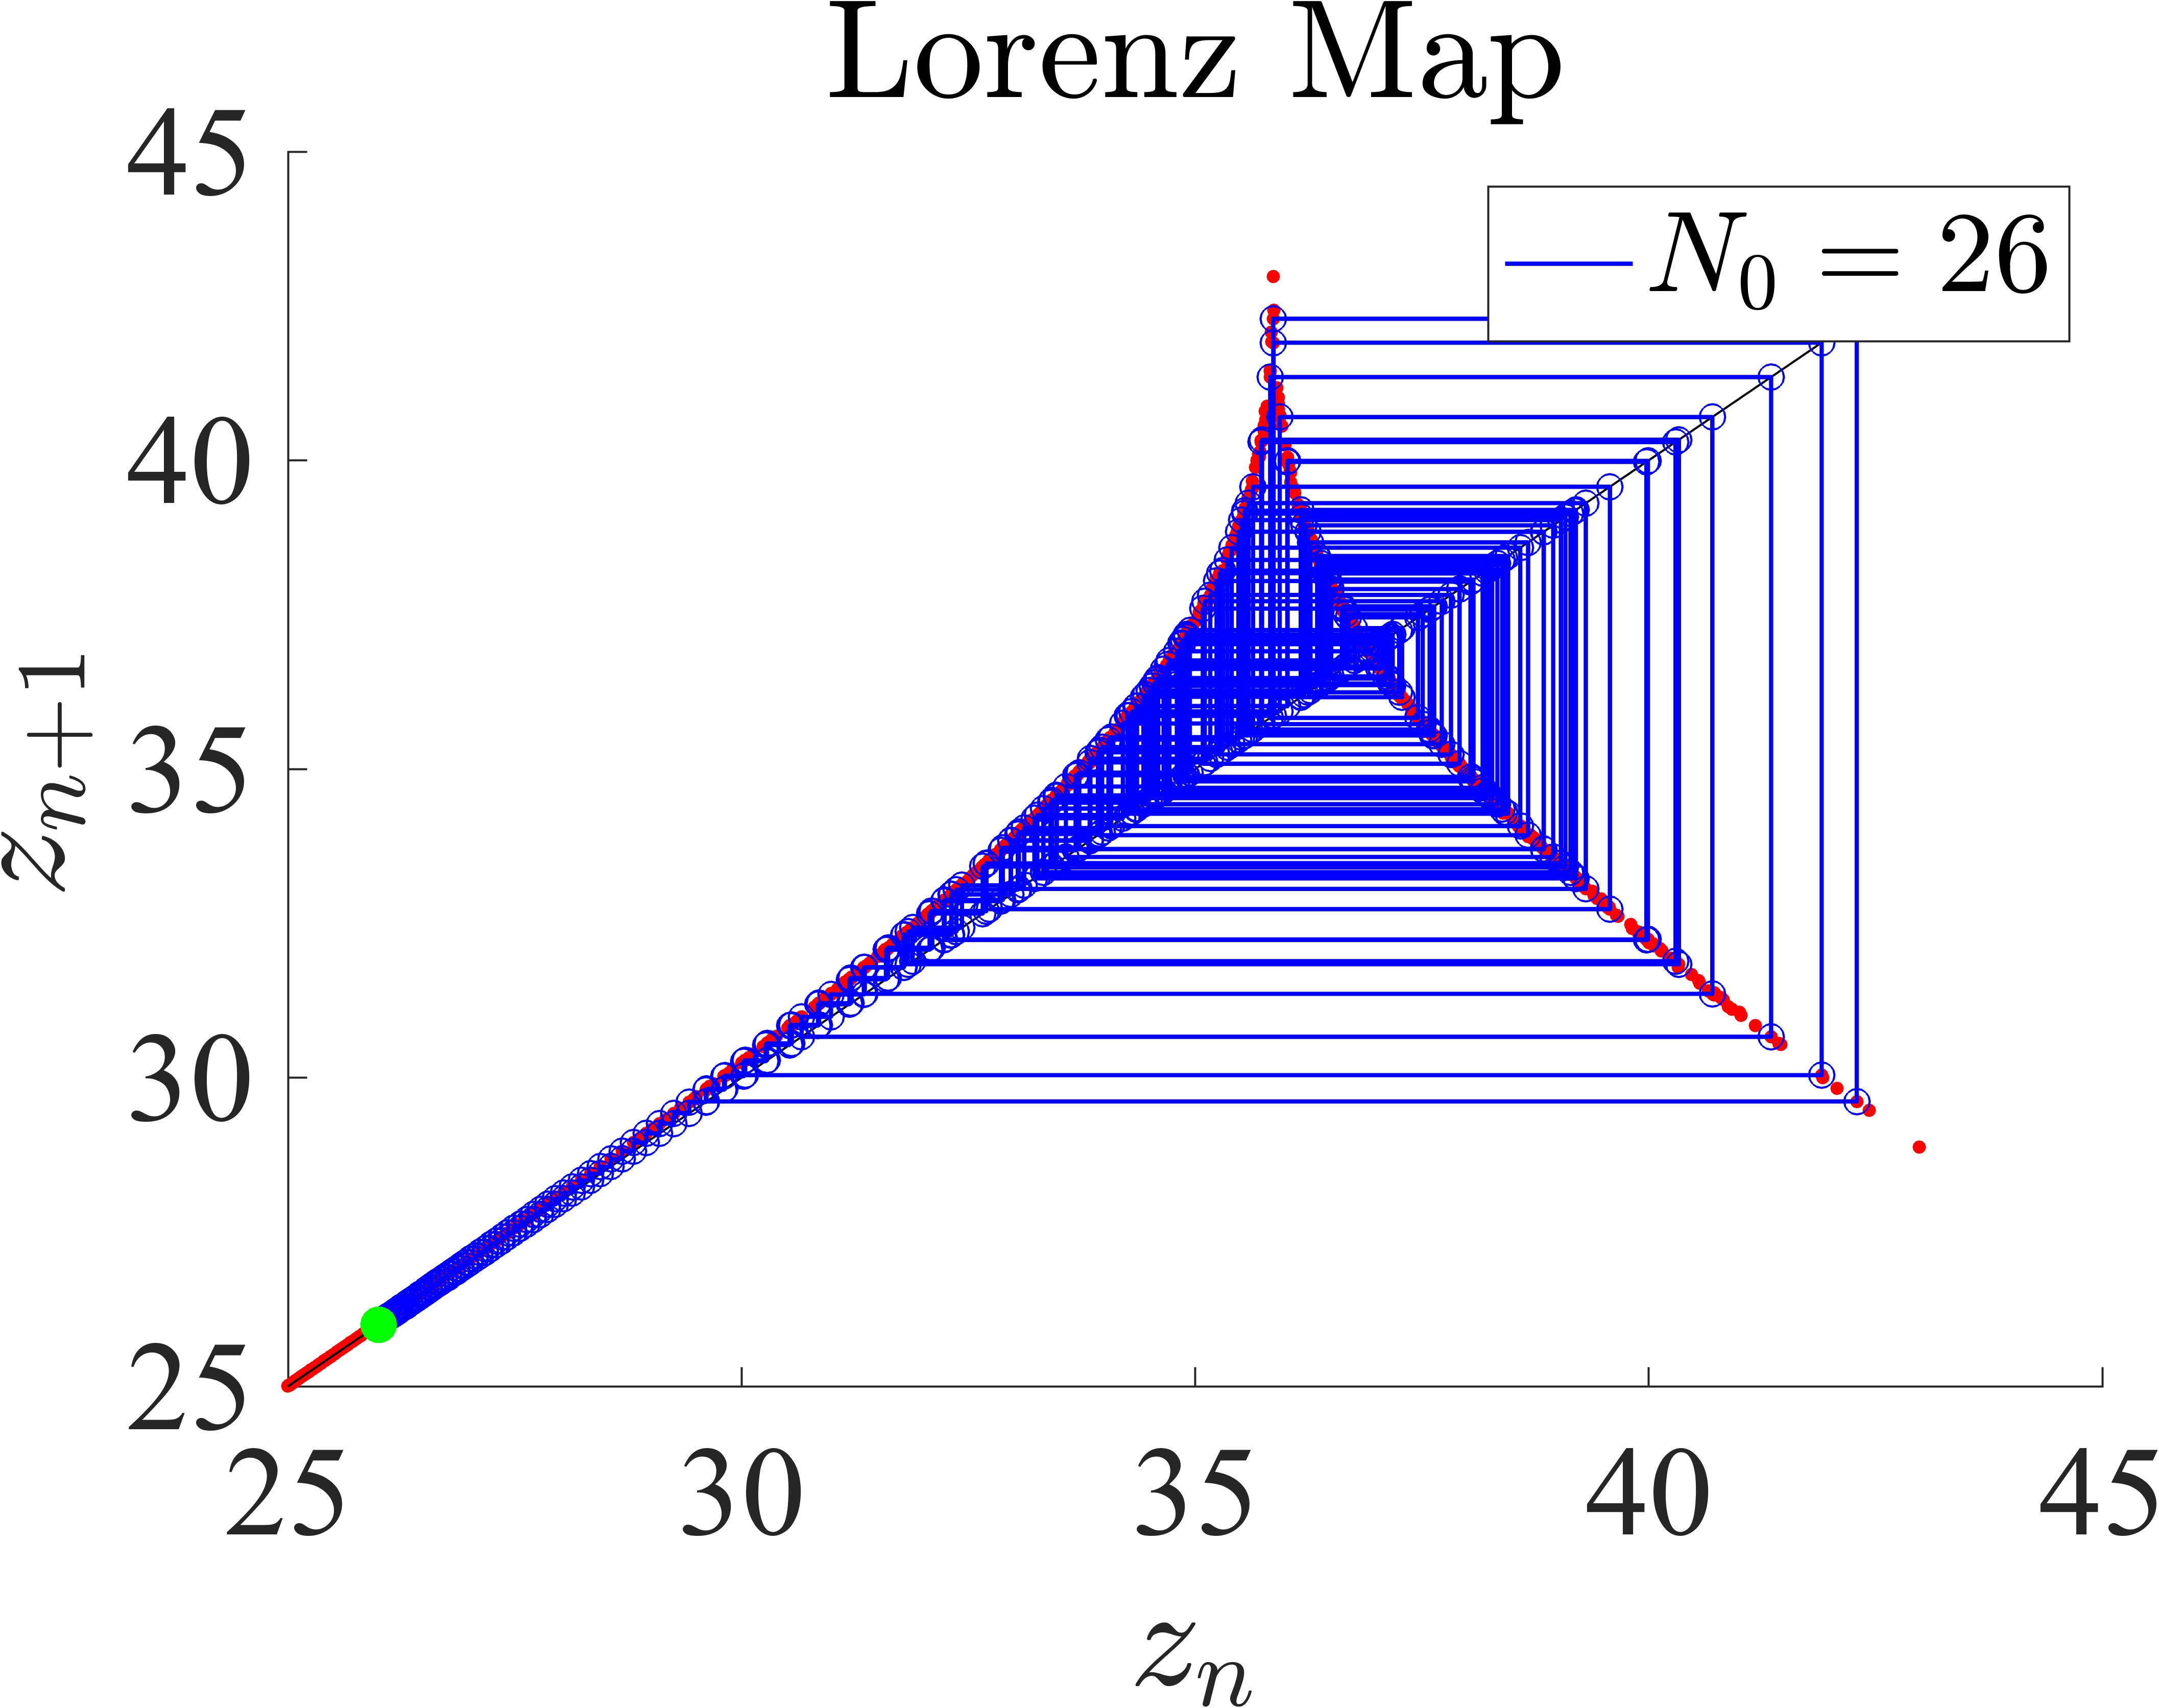
\includegraphics[width=8cm]{Lorenz_map_cobwebs_No26.png}
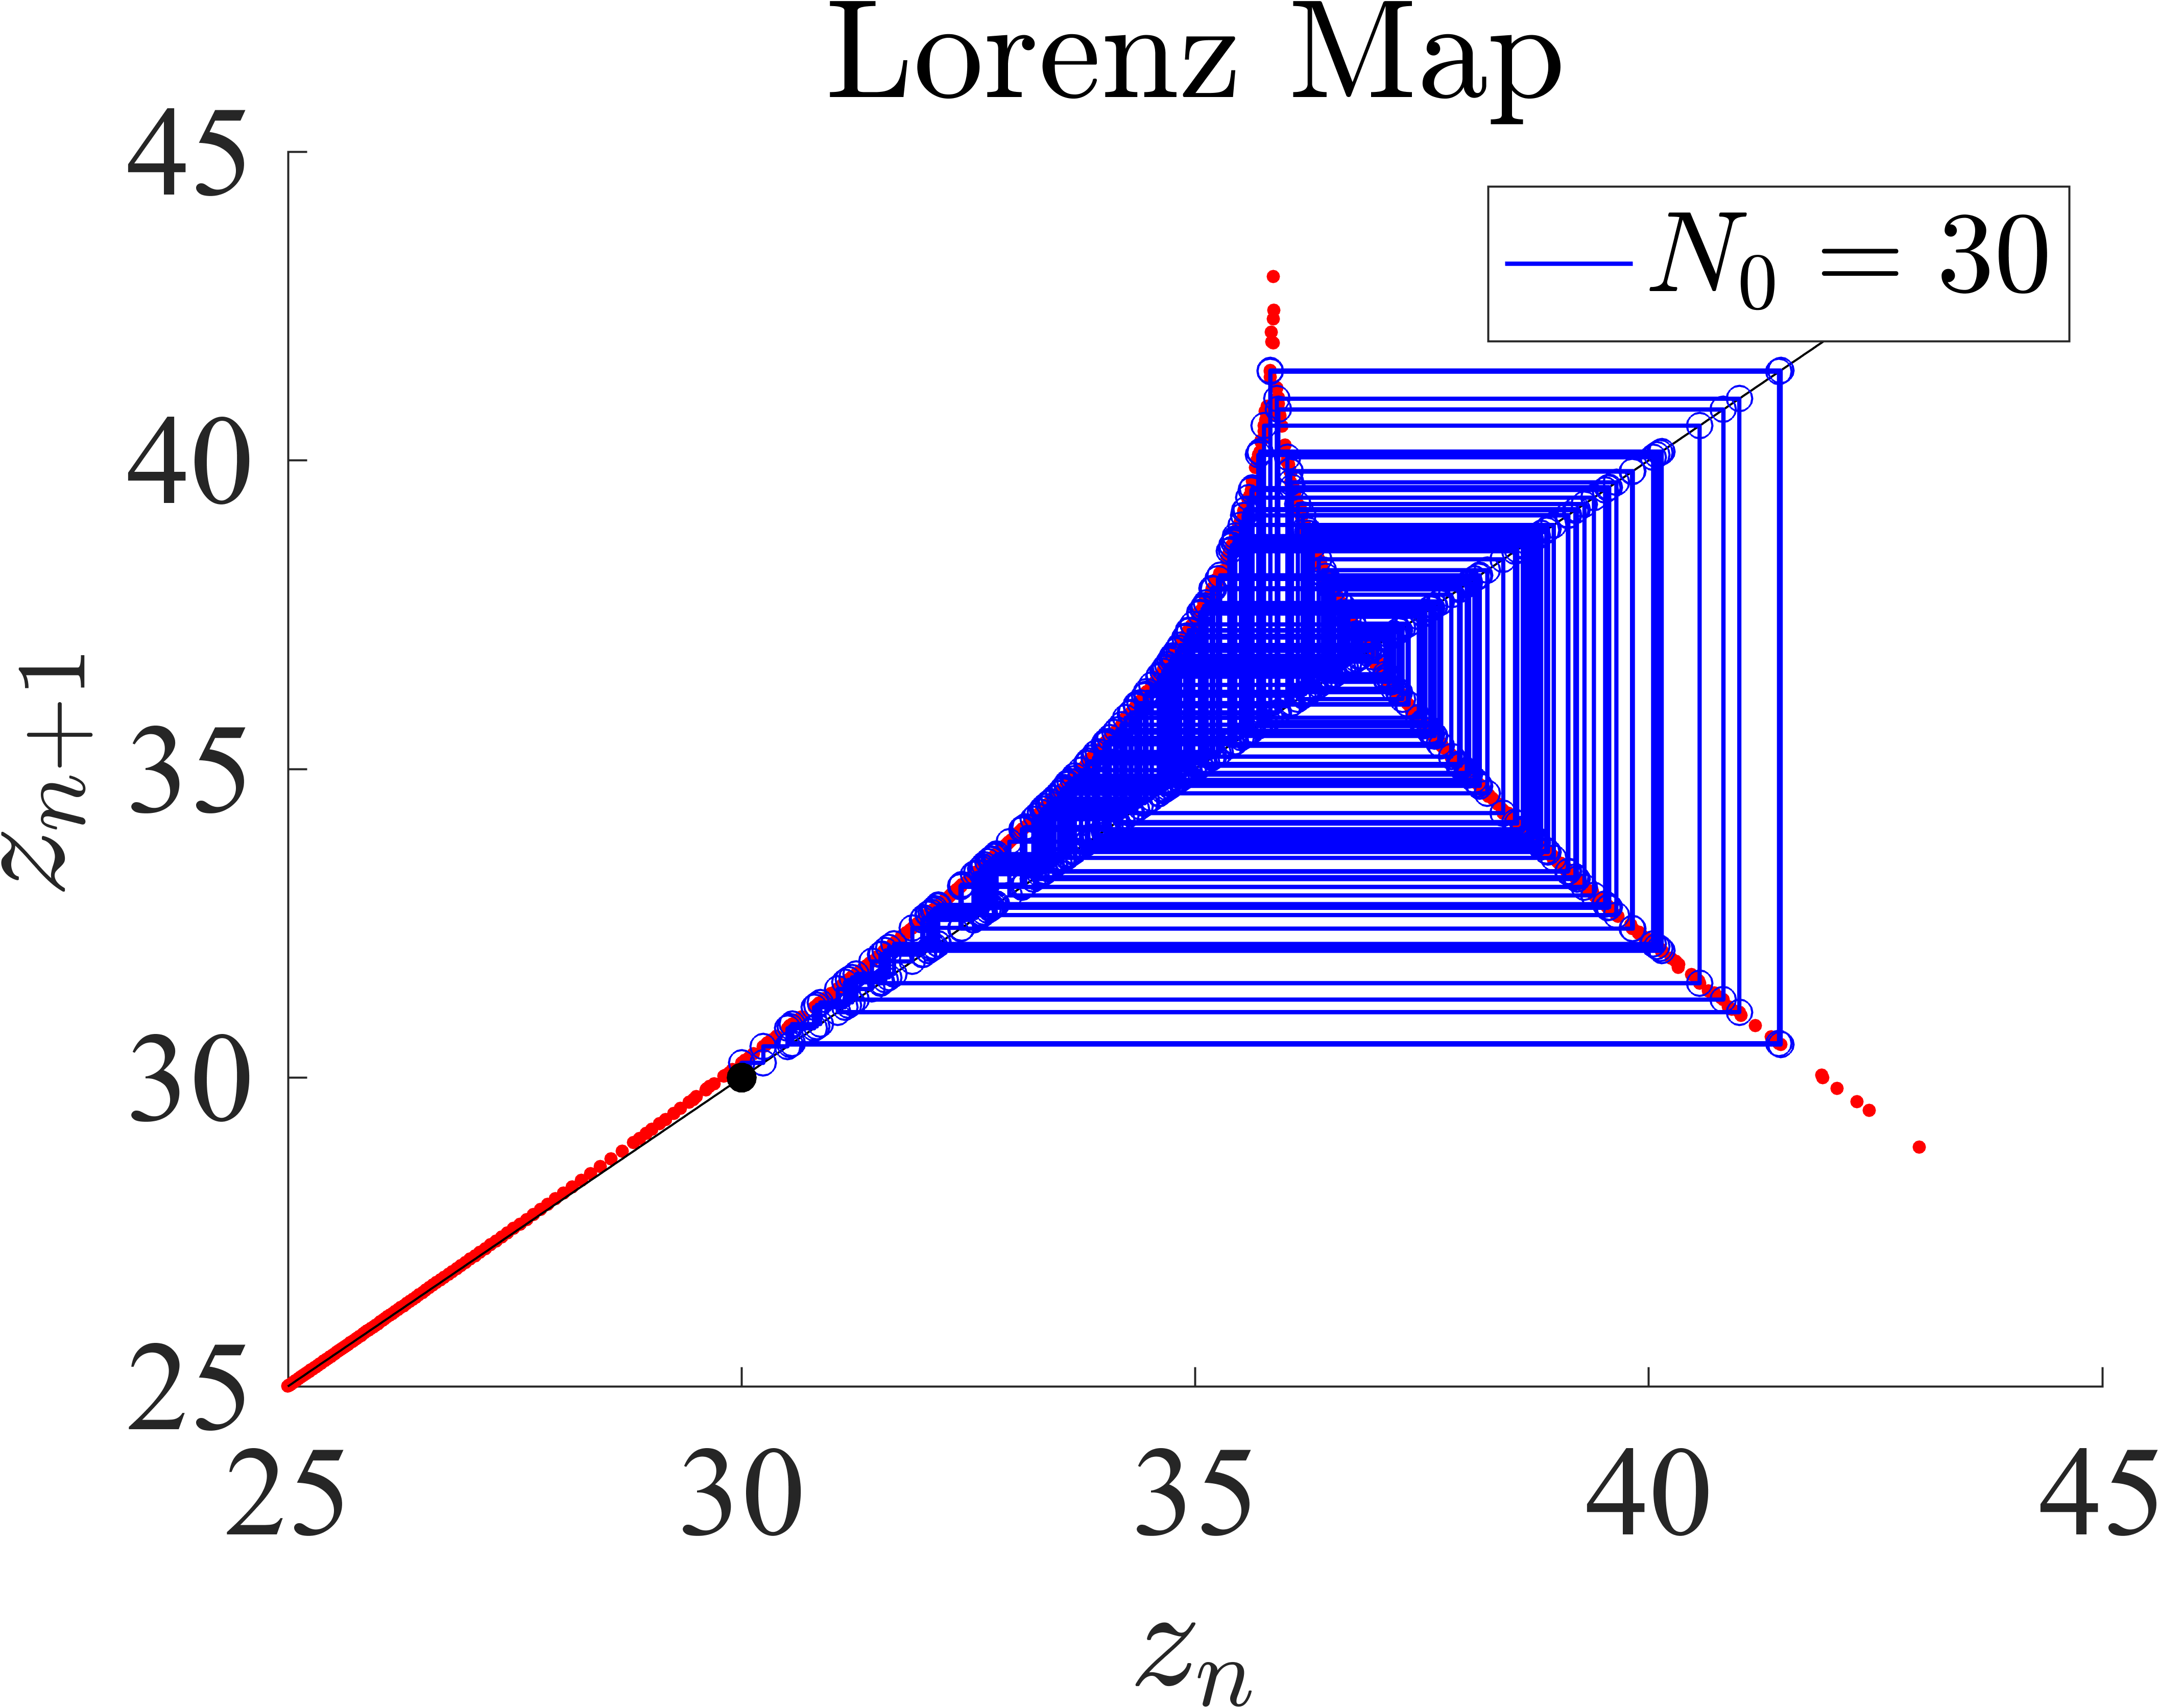
\includegraphics[width=8cm]{Lorenz_map_cobwebs_No30.png}
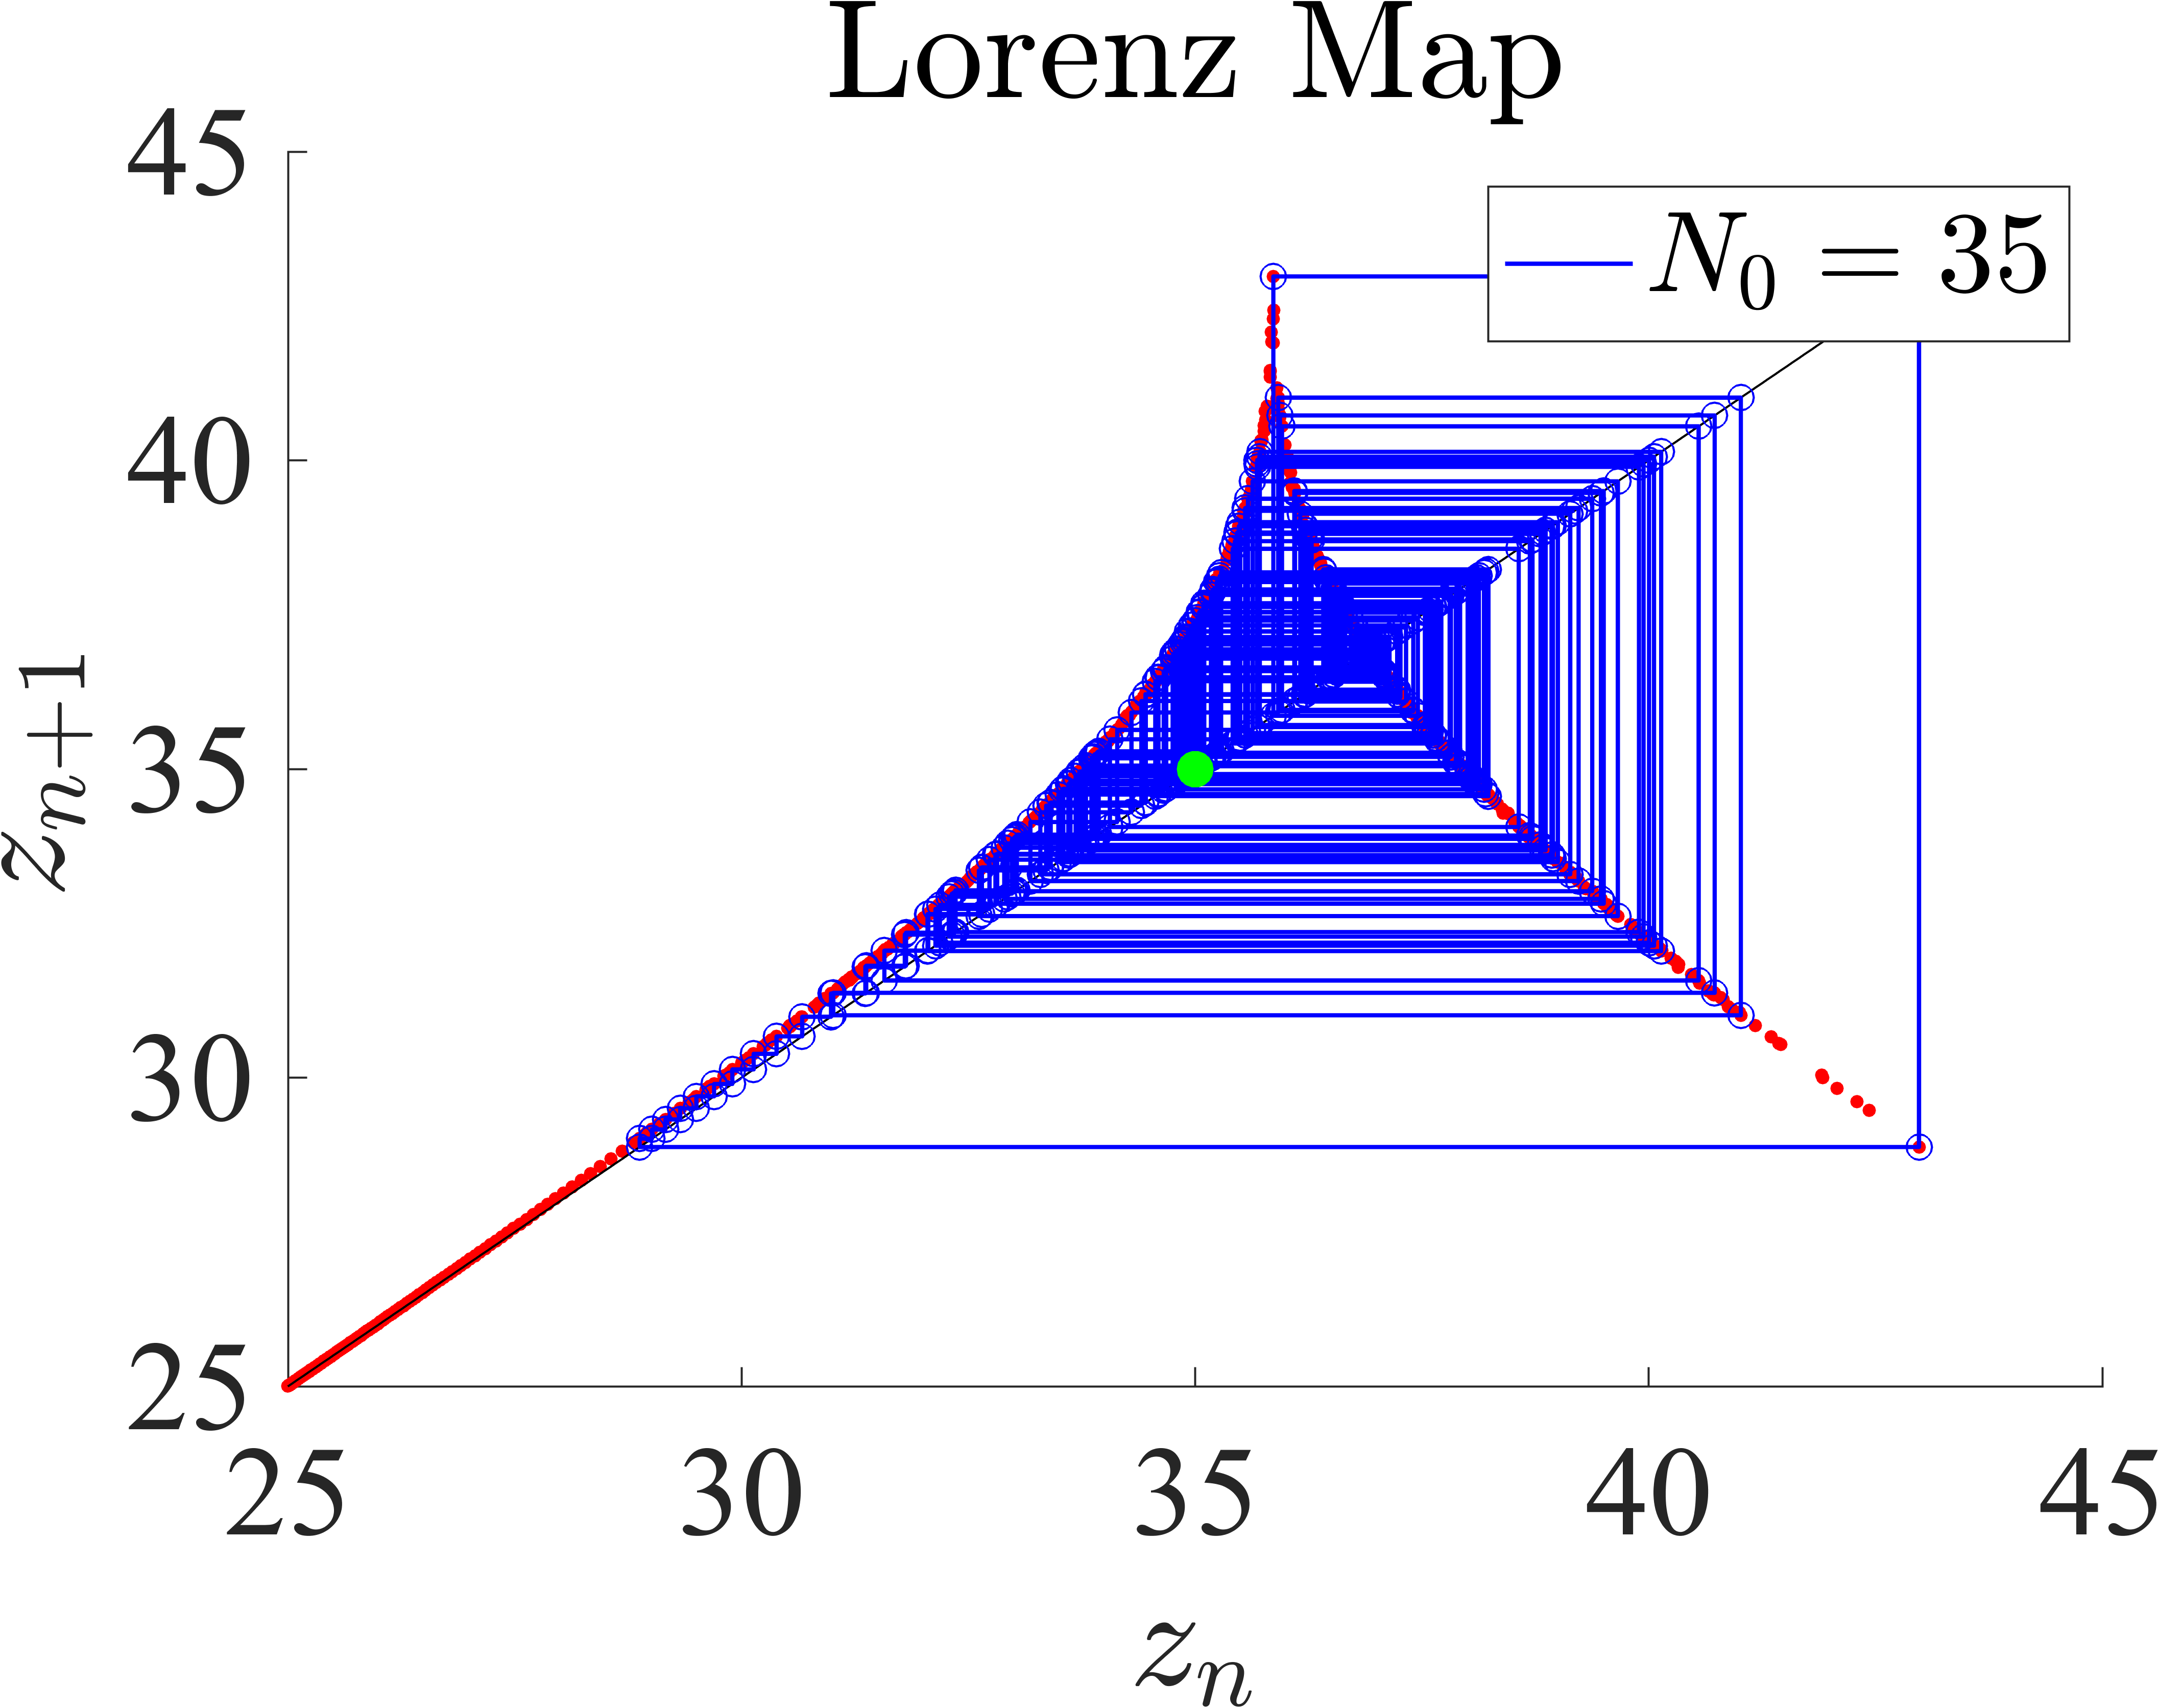
\includegraphics[width=8cm]{Lorenz_map_cobwebs_No35.png}
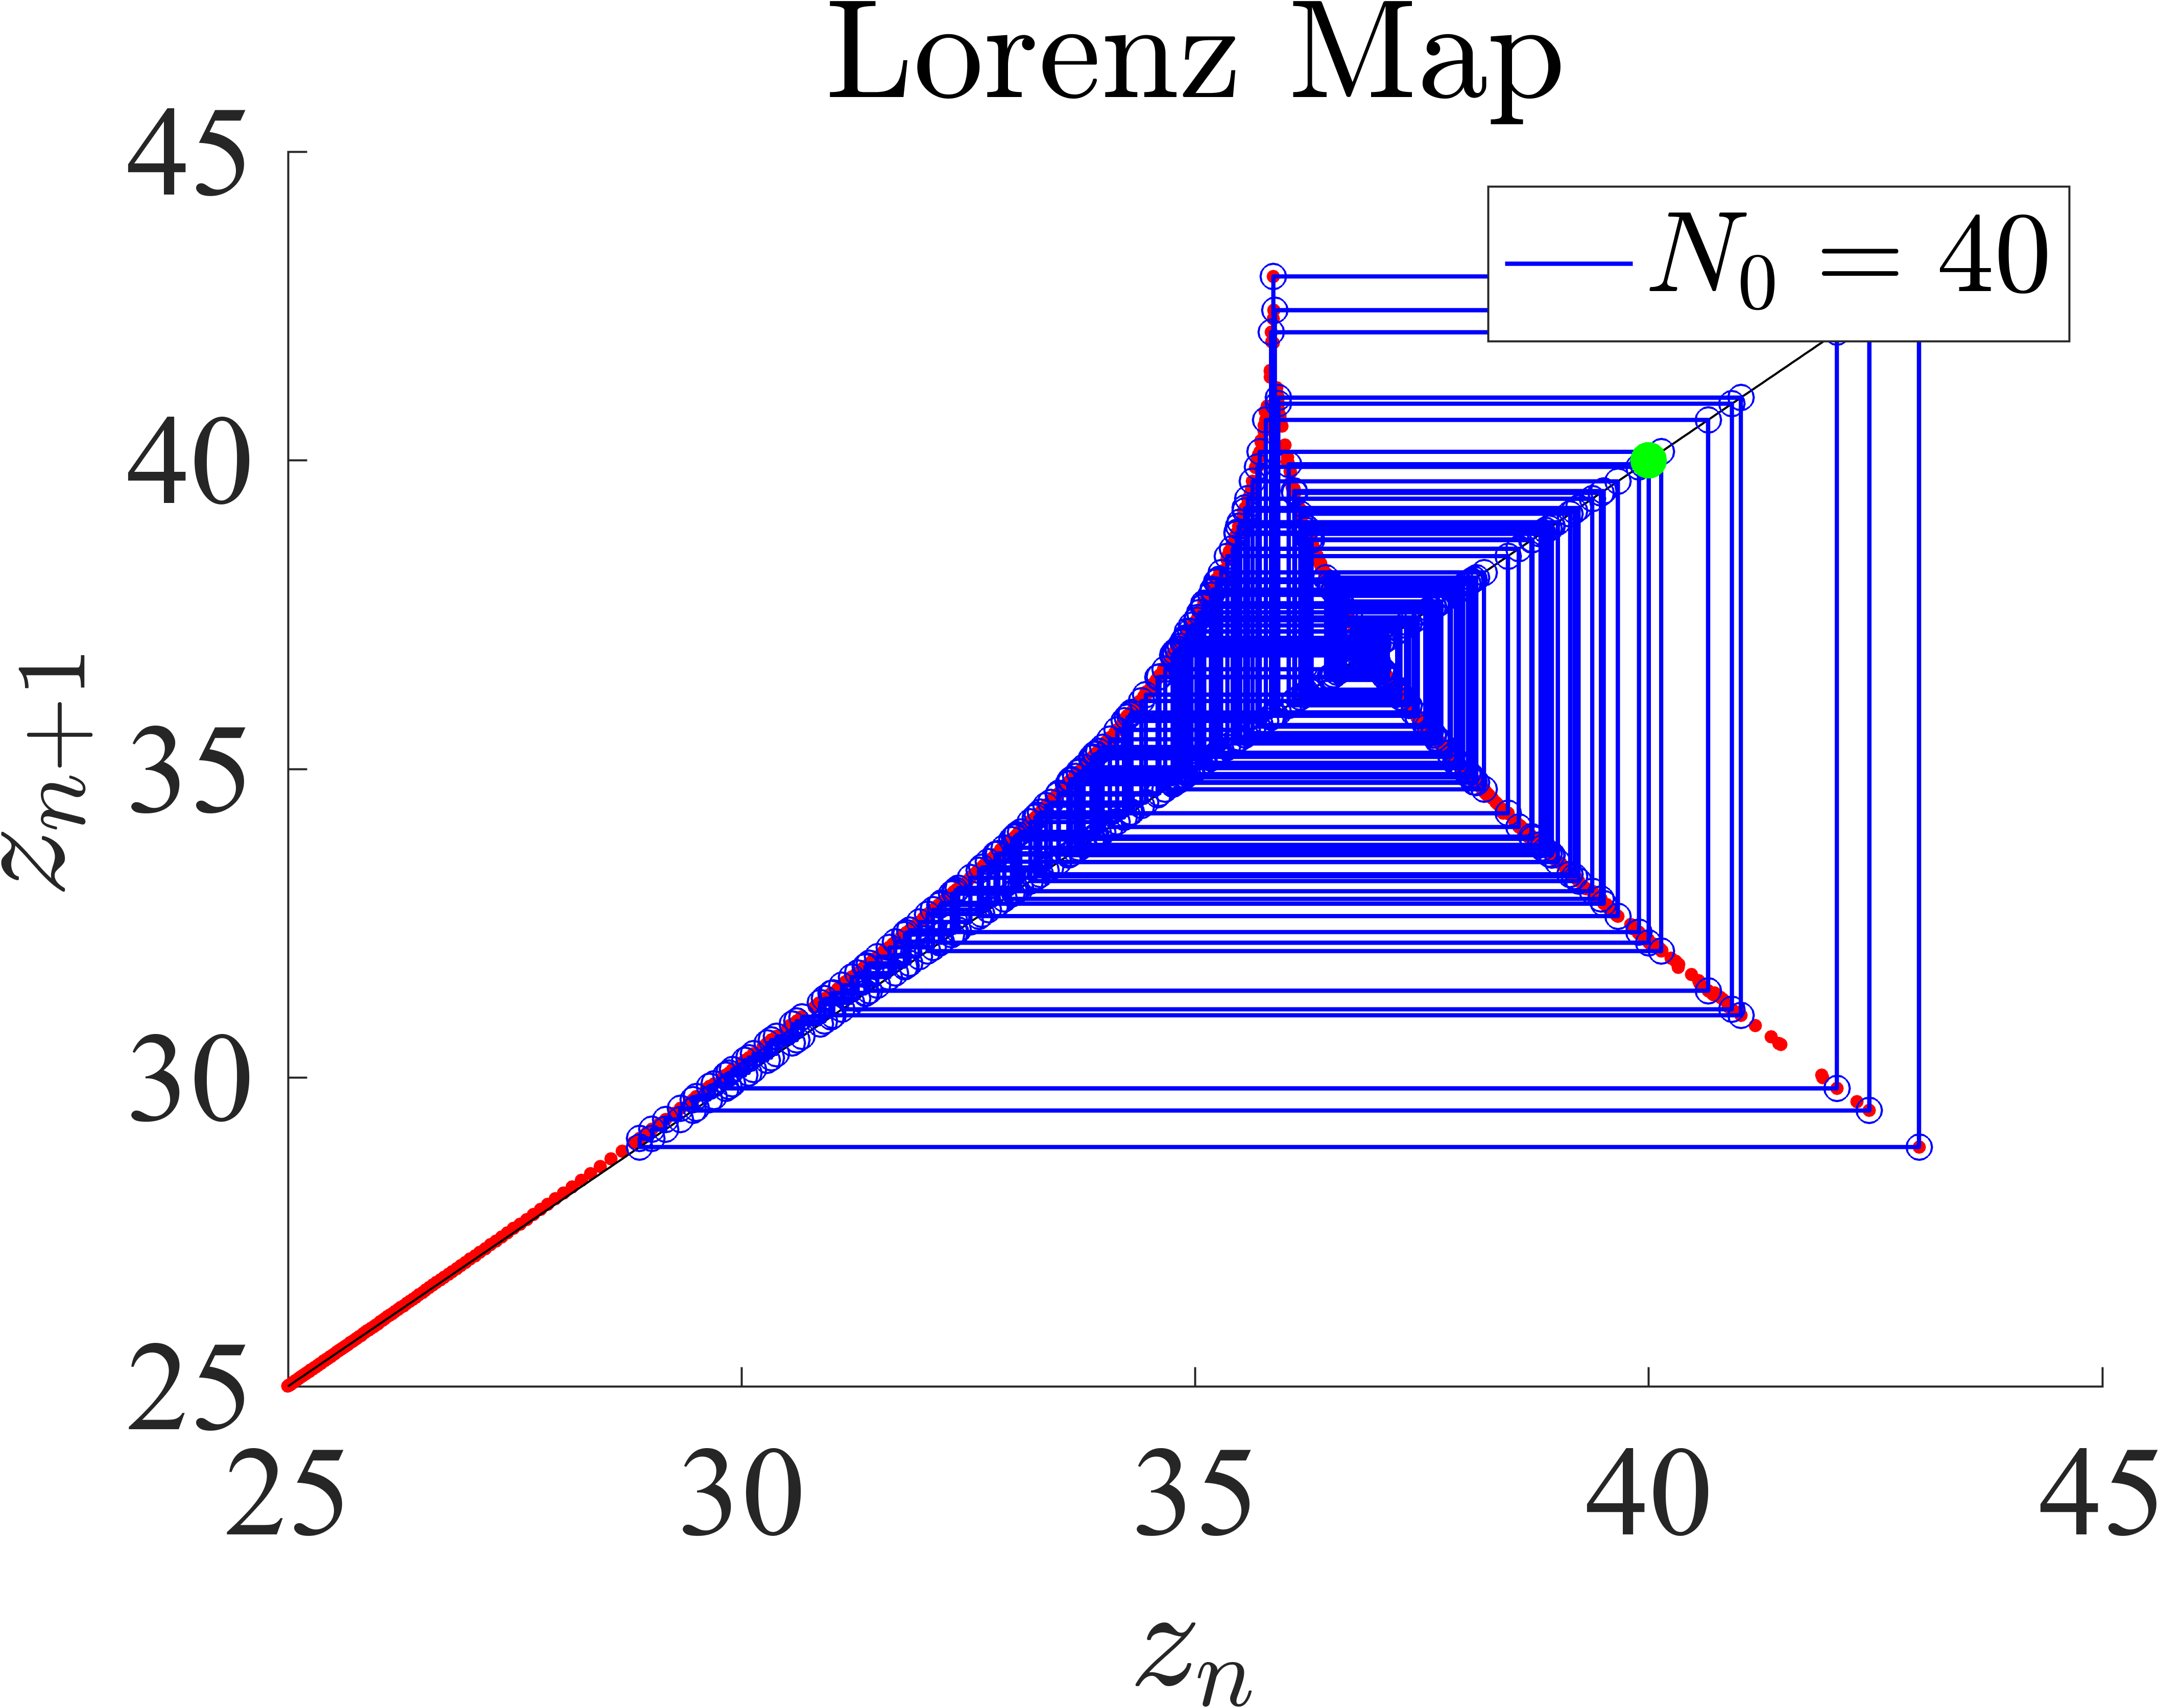
\includegraphics[width=8cm]{Lorenz_map_cobwebs_No40.png}
\caption{Lorenz Map Cobweb Diagrams, 500 Steps}
\end{figure}
\begin{figure}[h]
\centering
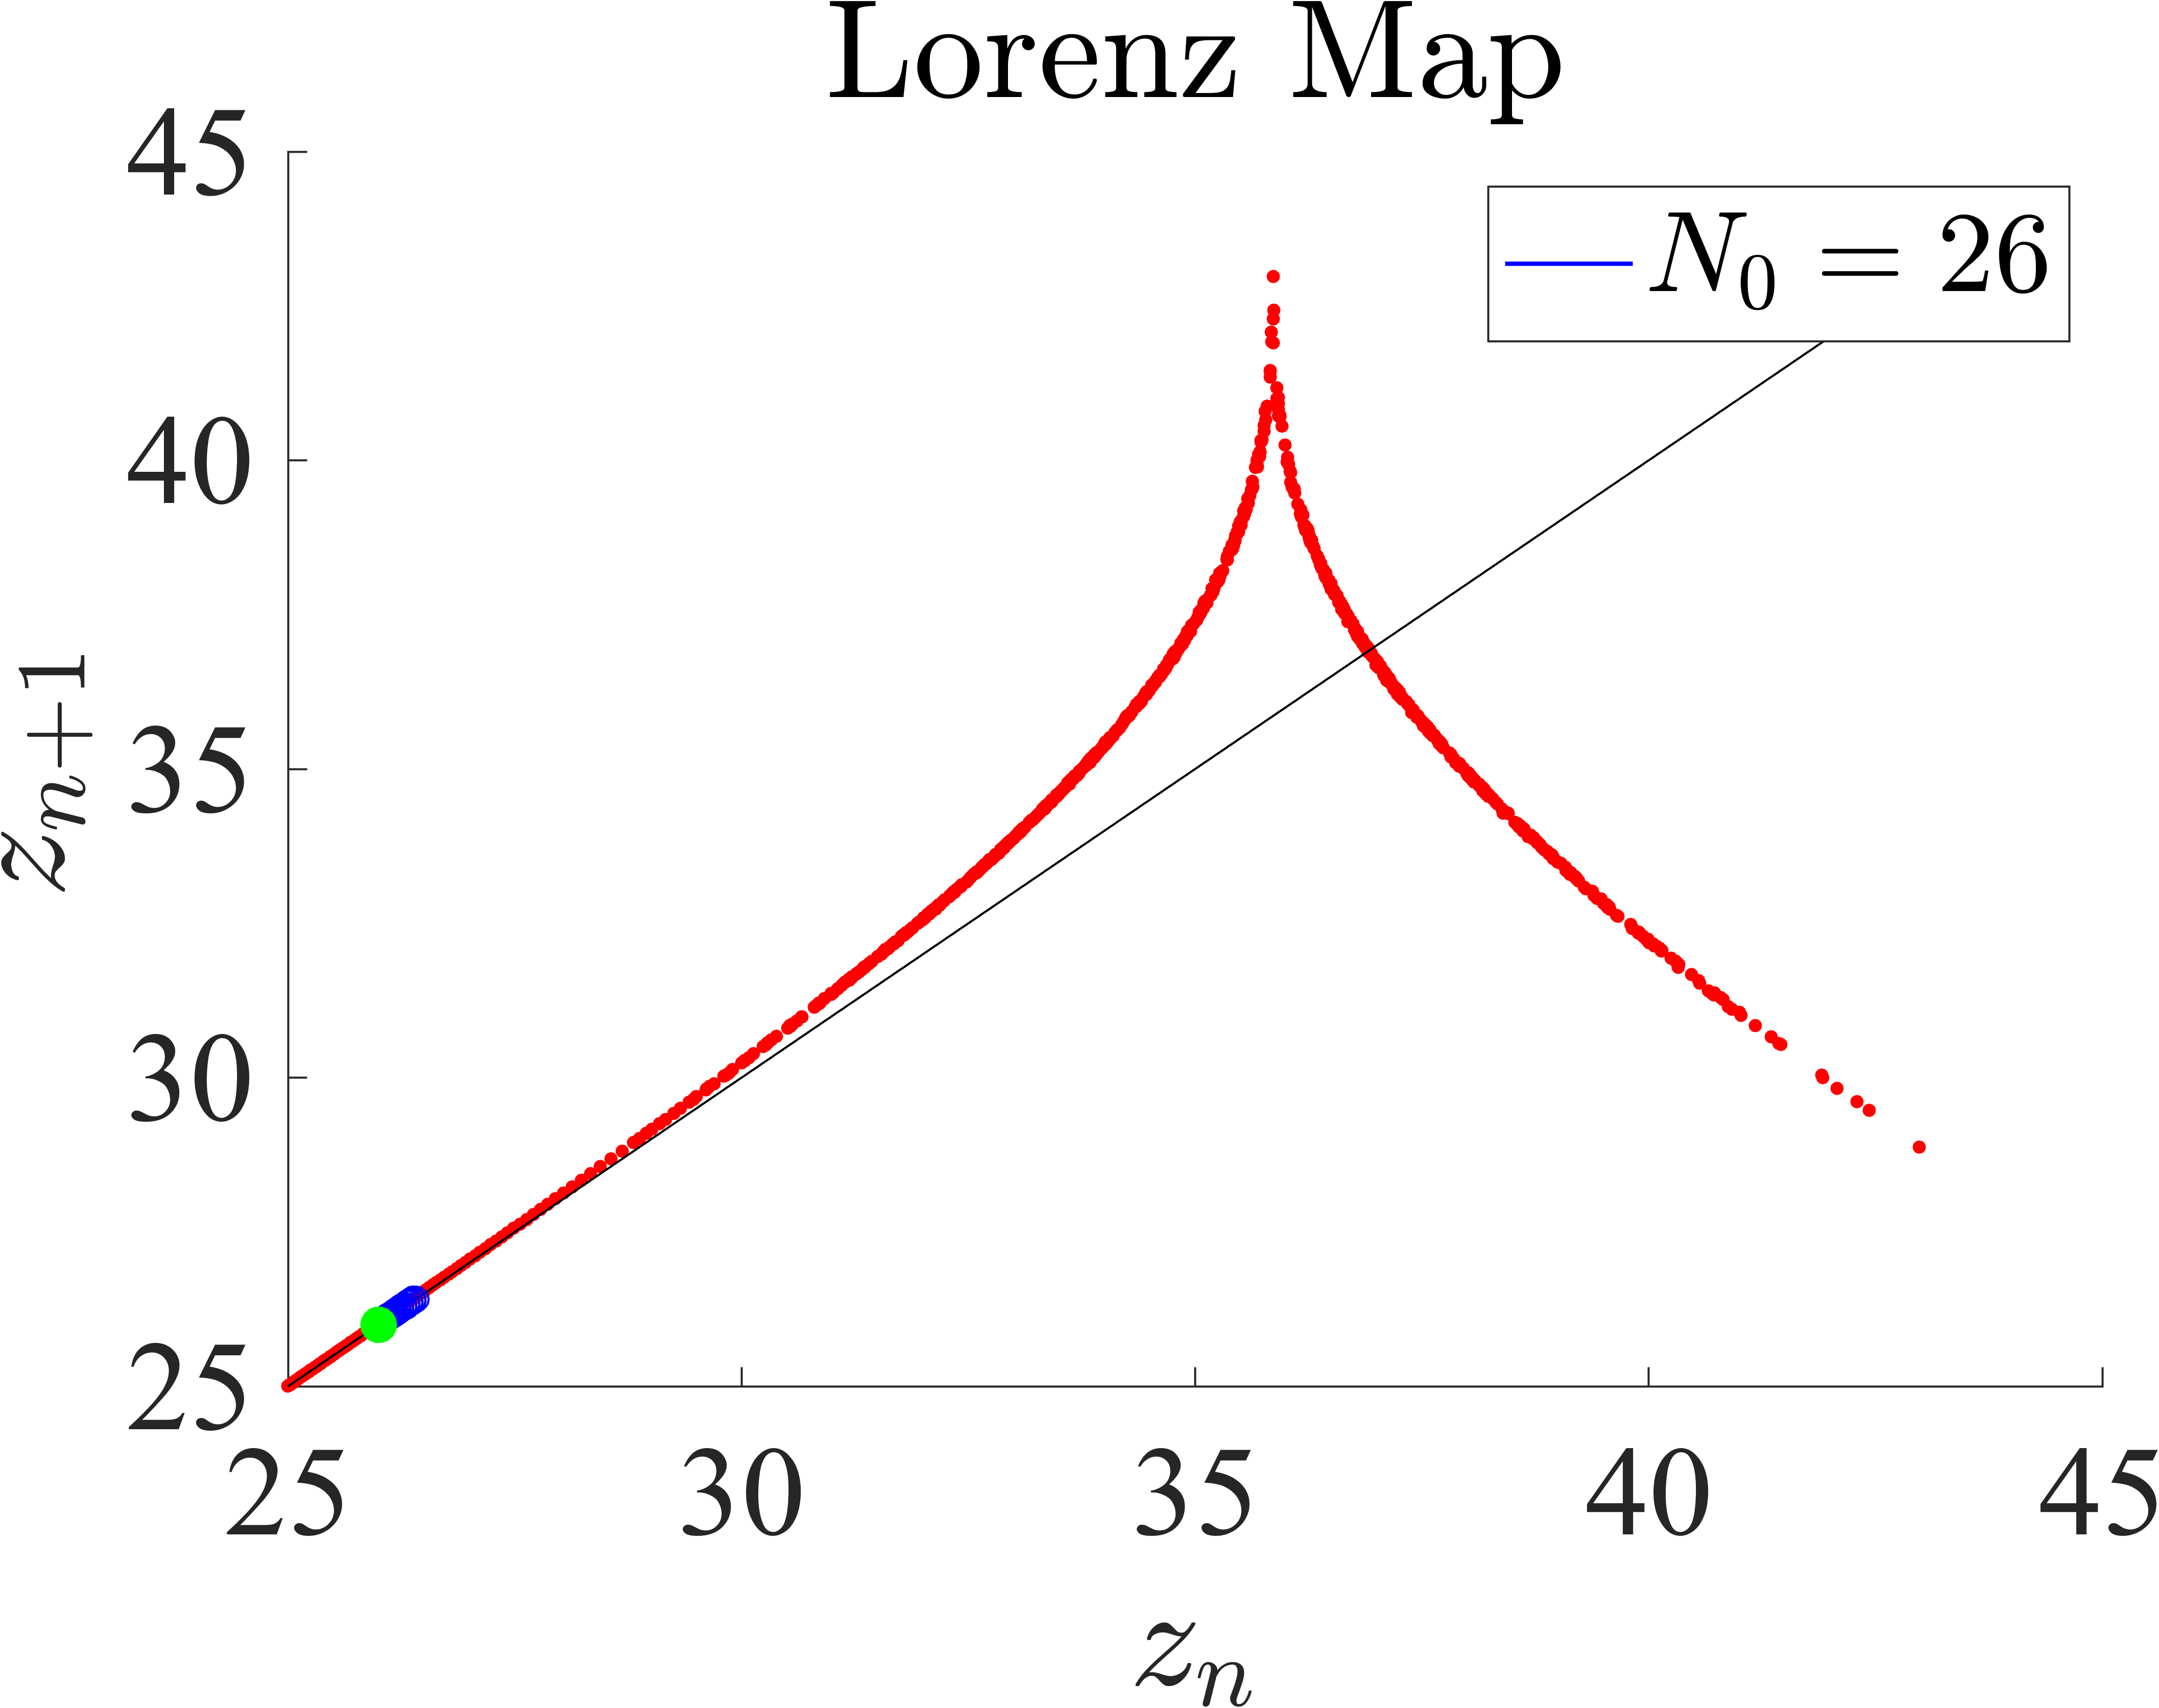
\includegraphics[width=8cm]{Lorenz_map_cobwebs_No26_ld.png}
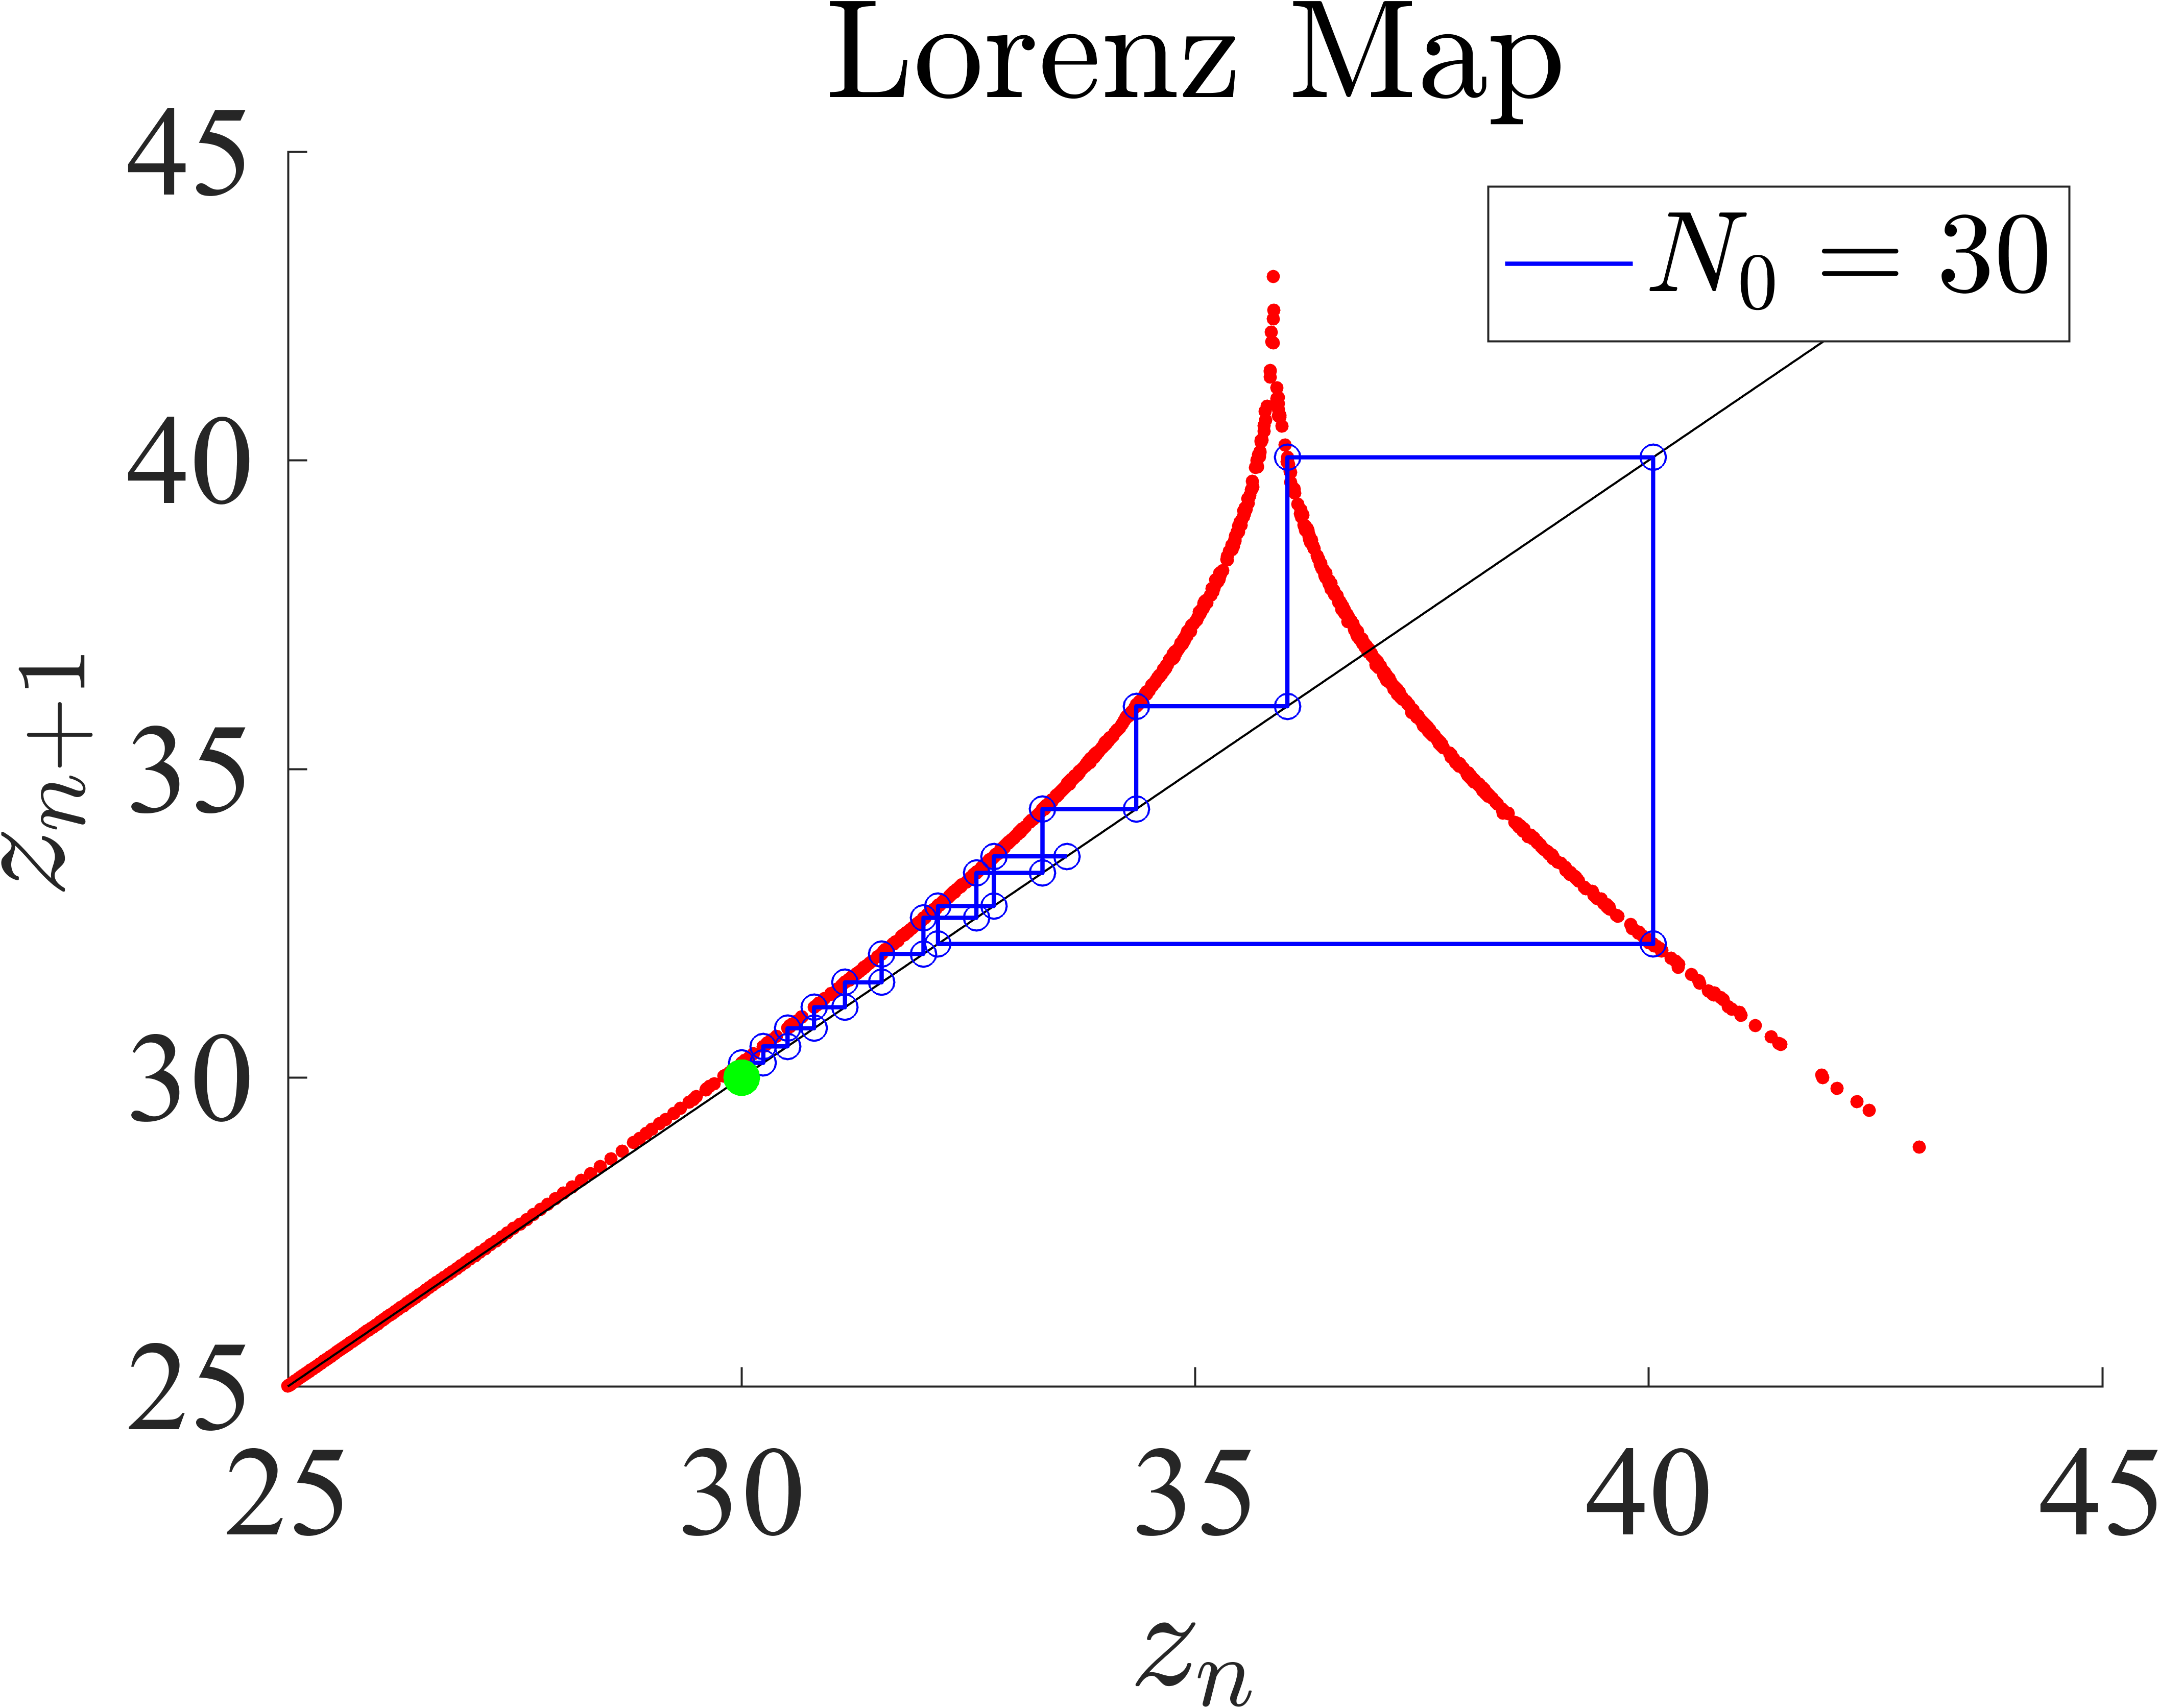
\includegraphics[width=8cm]{Lorenz_map_cobwebs_No30_ld.png}
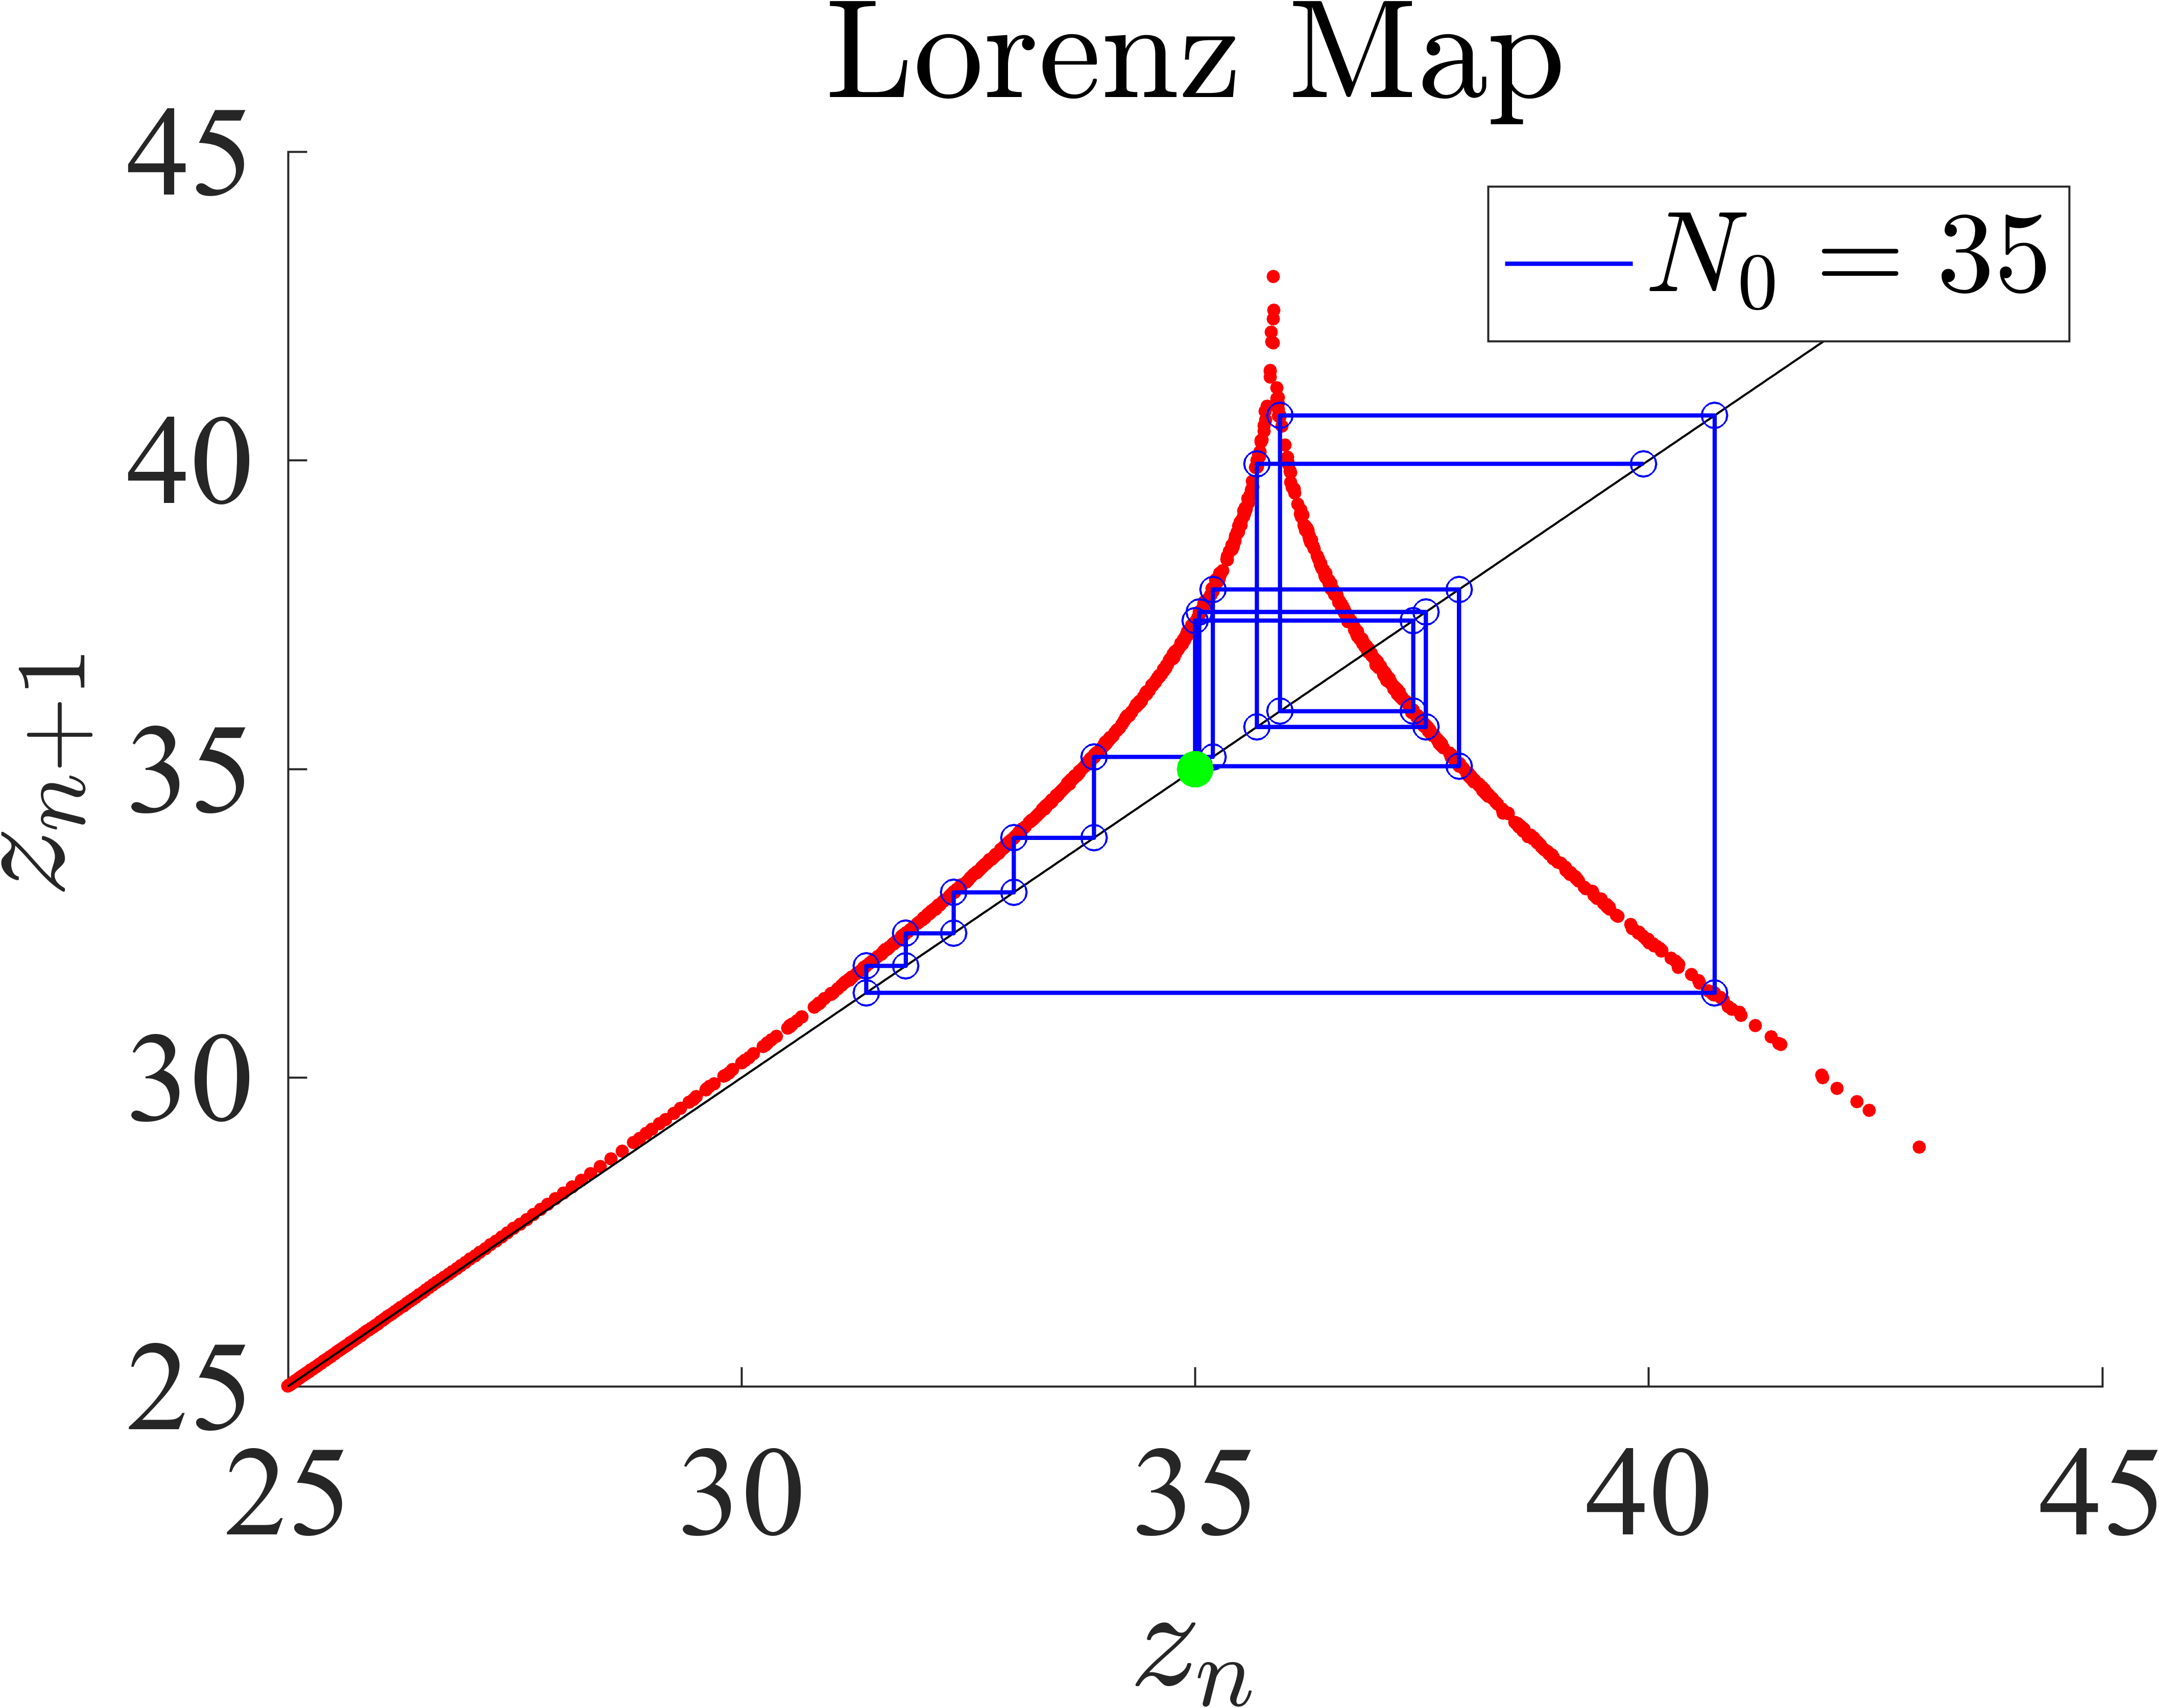
\includegraphics[width=8cm]{Lorenz_map_cobwebs_No35_ld.png}
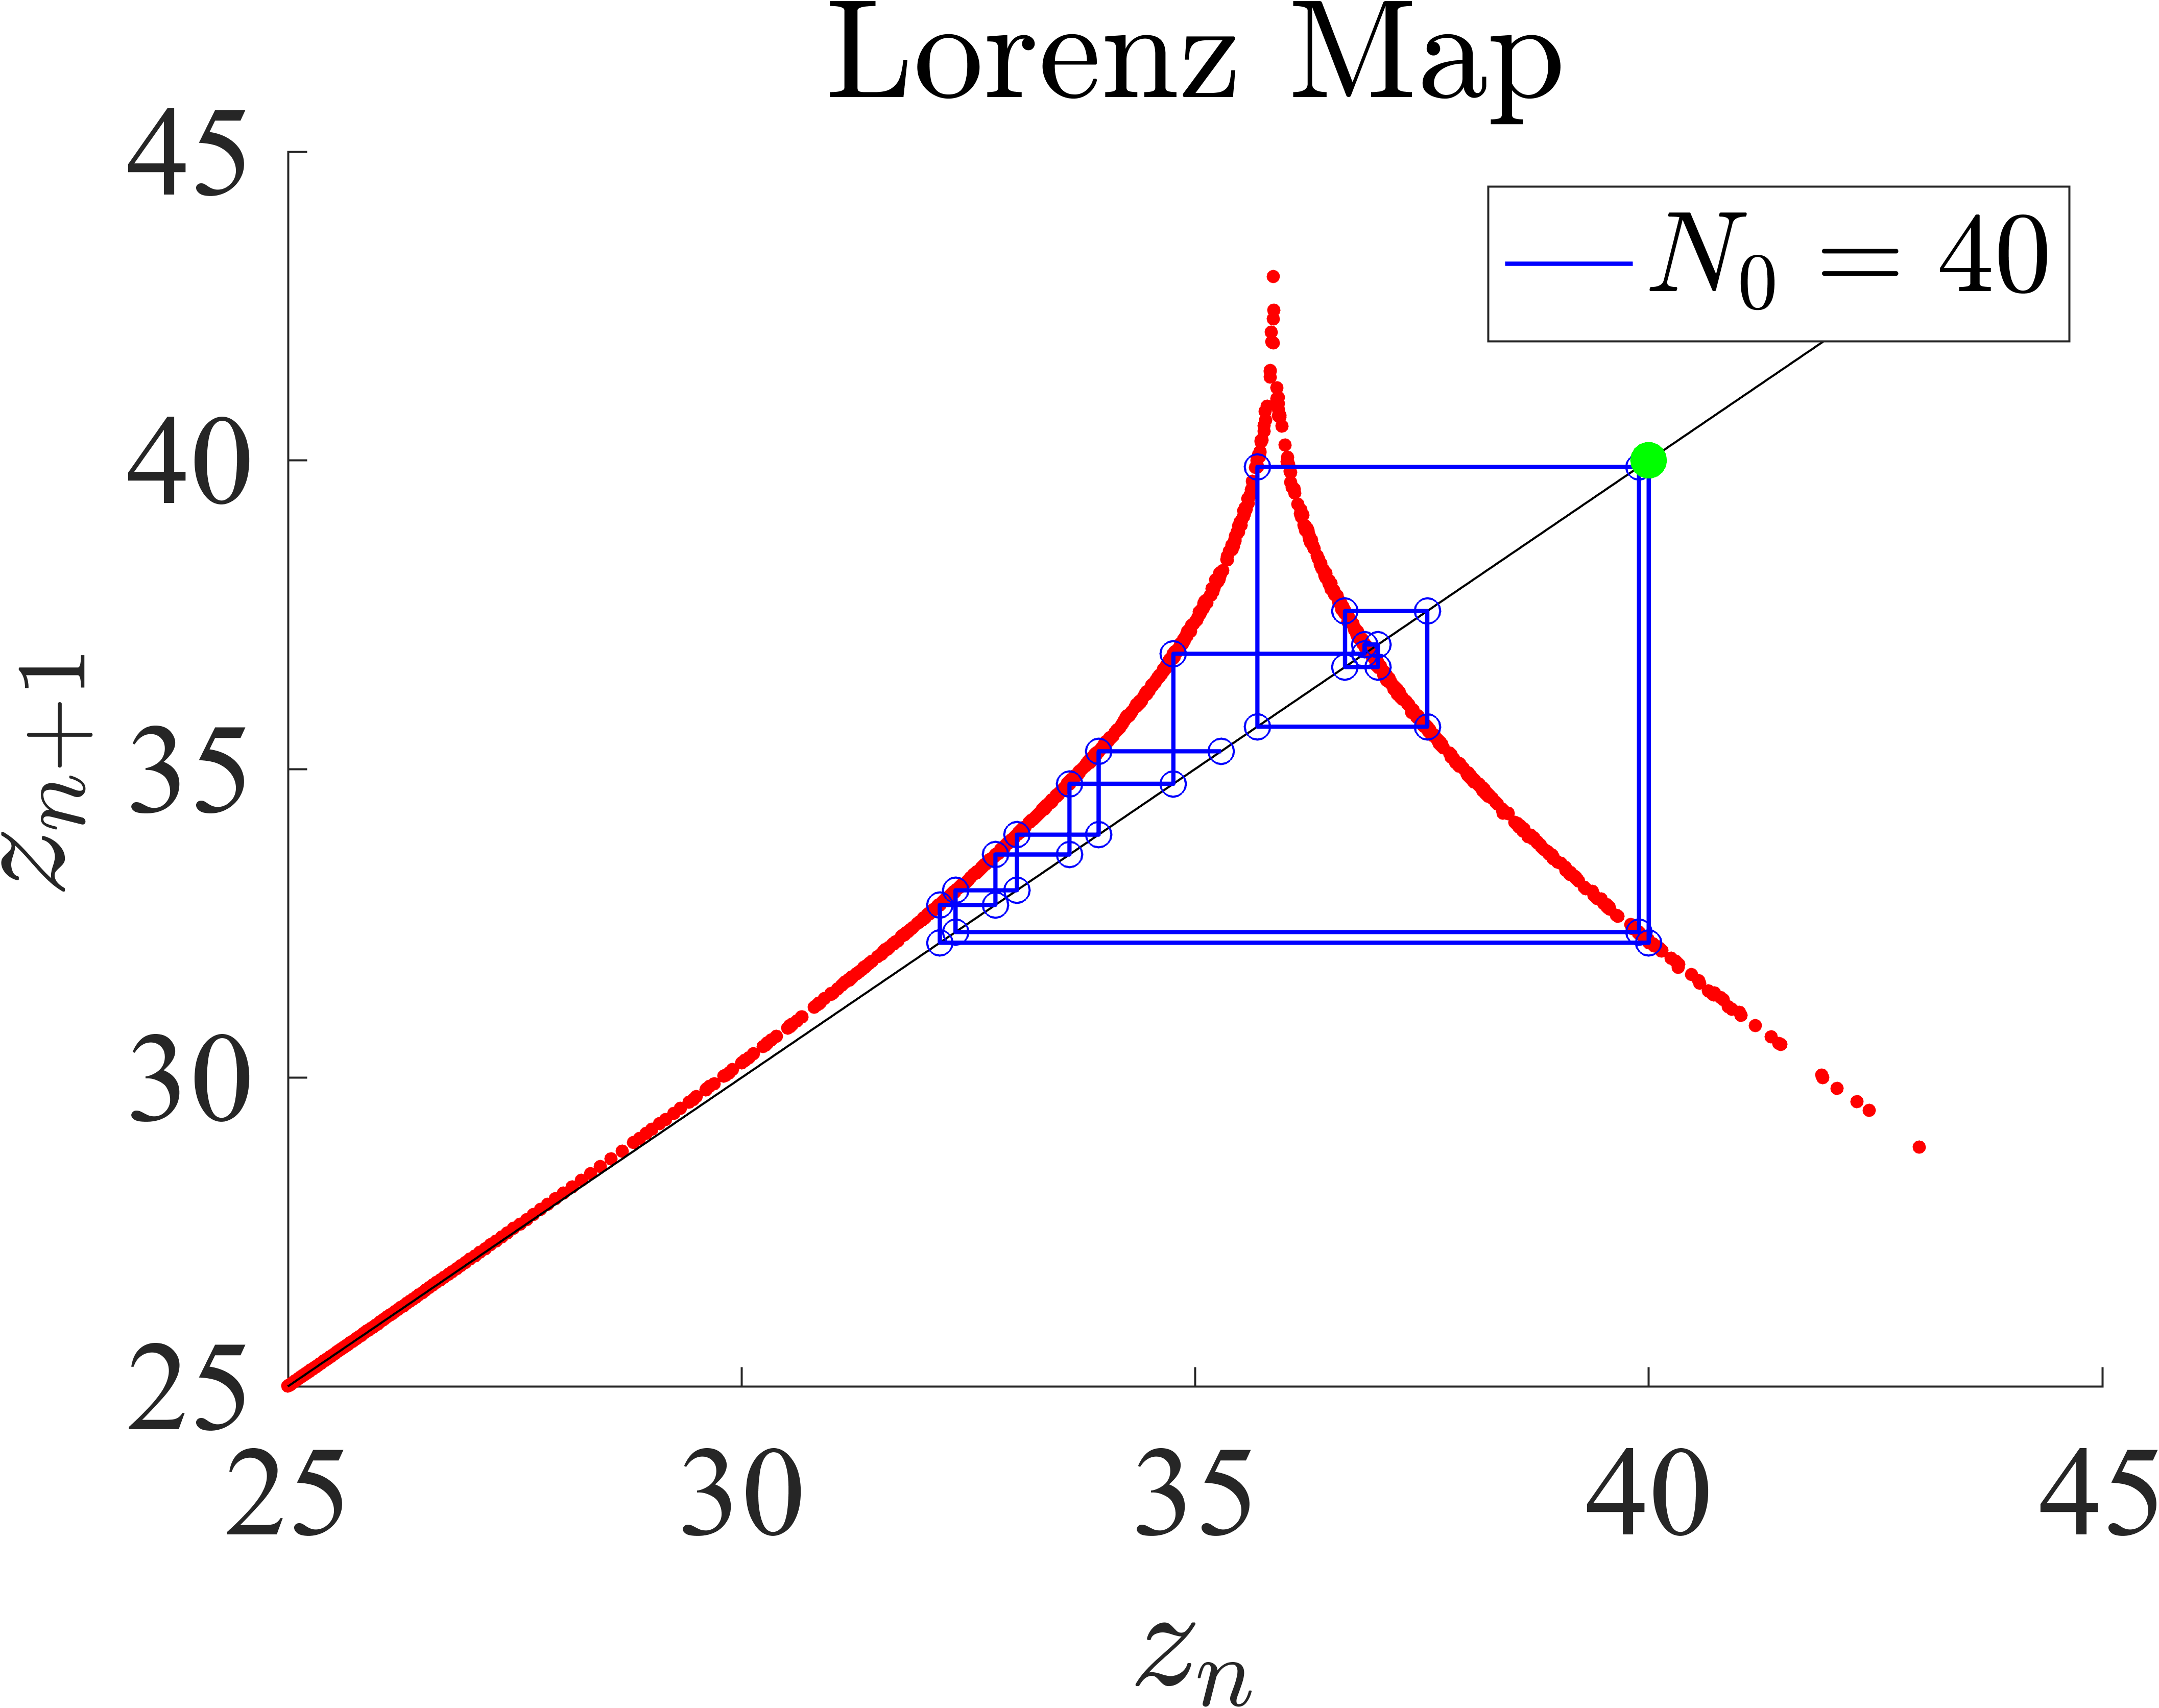
\includegraphics[width=8cm]{Lorenz_map_cobwebs_No40_ld.png}
\caption{Lorenz Map Cobweb Diagrams, 30 Steps}
\end{figure}

\clearpage
\section*{Maps and Period Doubling}
Here I run a recursion for the logistic map ($x_{n+1} = rx_n(1-x_n)$) and the sine map ($x_{n+1} = r\sin(\pi x_n)$) for different values of $r$. For the logistic map, I sample $r$ ranging from $3.4$ to $4.0$. For the sine map, I sample $r$ ranging from $0.5$ to $1.0$. I then plot the last 1,000 points for each simulation versus the corresponding value of $r$ to see where the map settles (as in an attractor). For both cases, we see an interesting structure in which the number of fixed points (or the number of lines) repeatedly doubles as $r$ increases. When $r$ reaches a critical value, it seems like there is no one fixed point and the solution becomes chaotic. 
\begin{figure}[h]
\centering
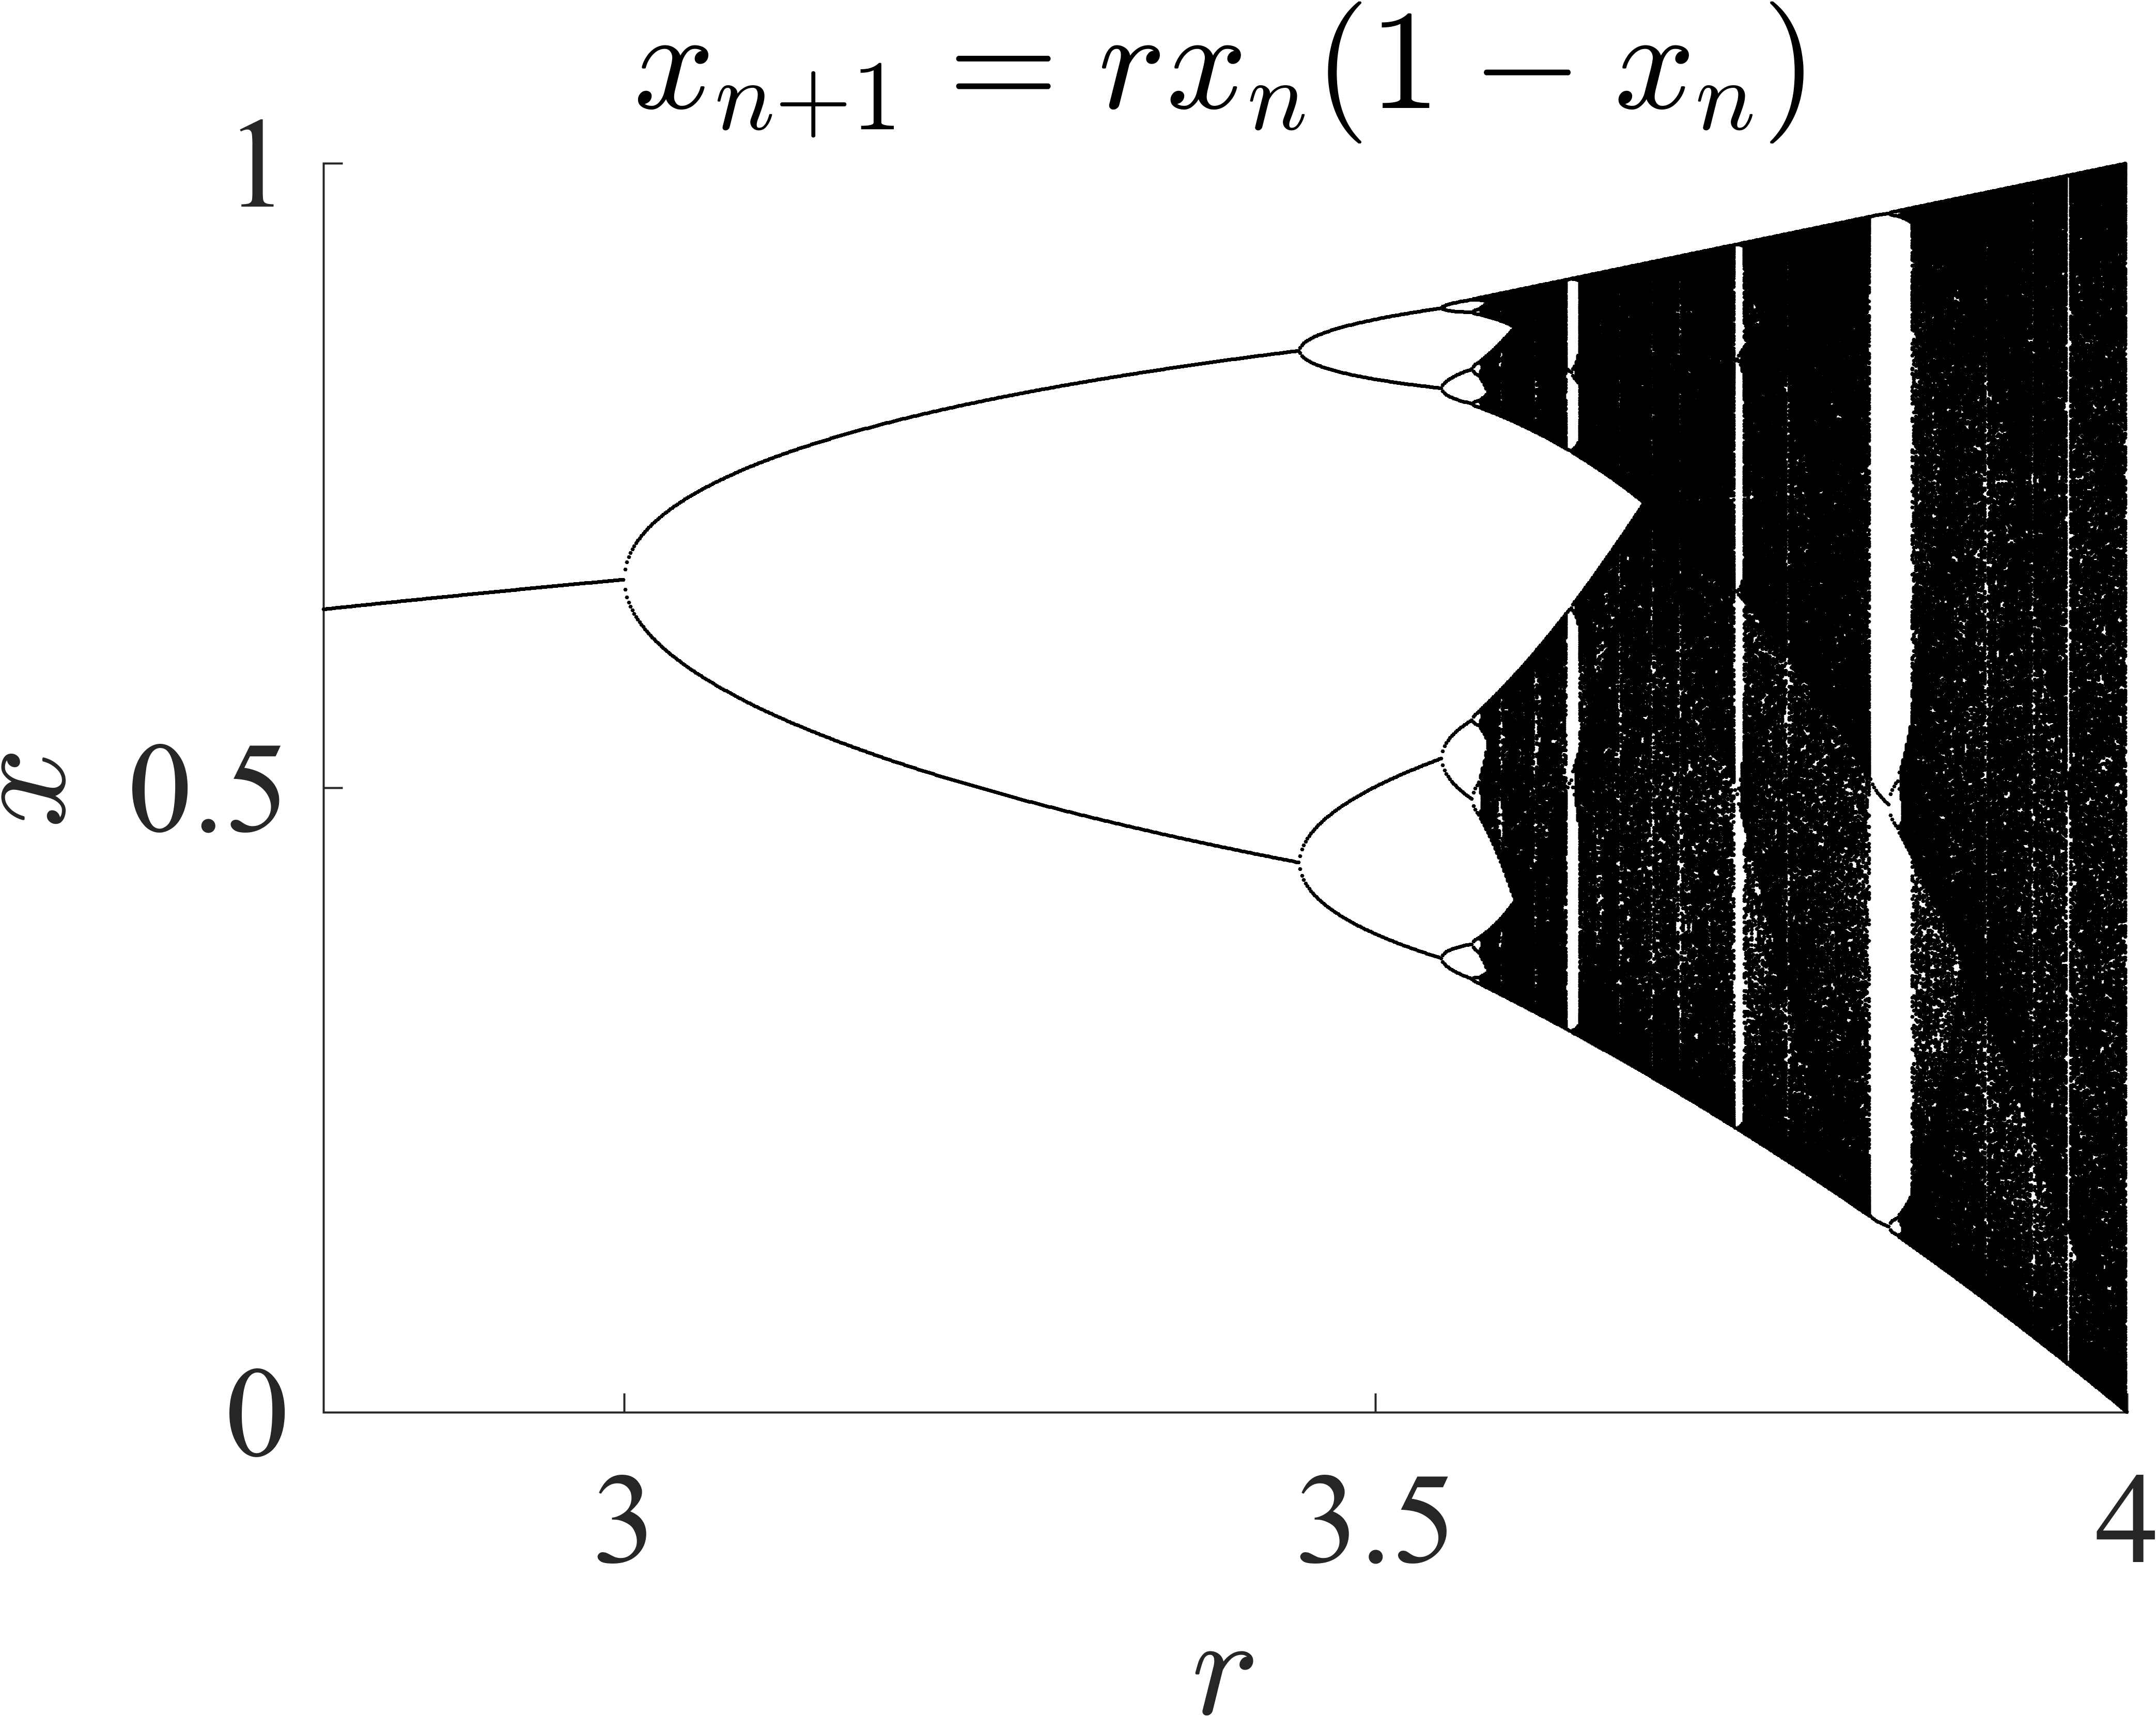
\includegraphics[width=8cm]{Logistic_map.png}
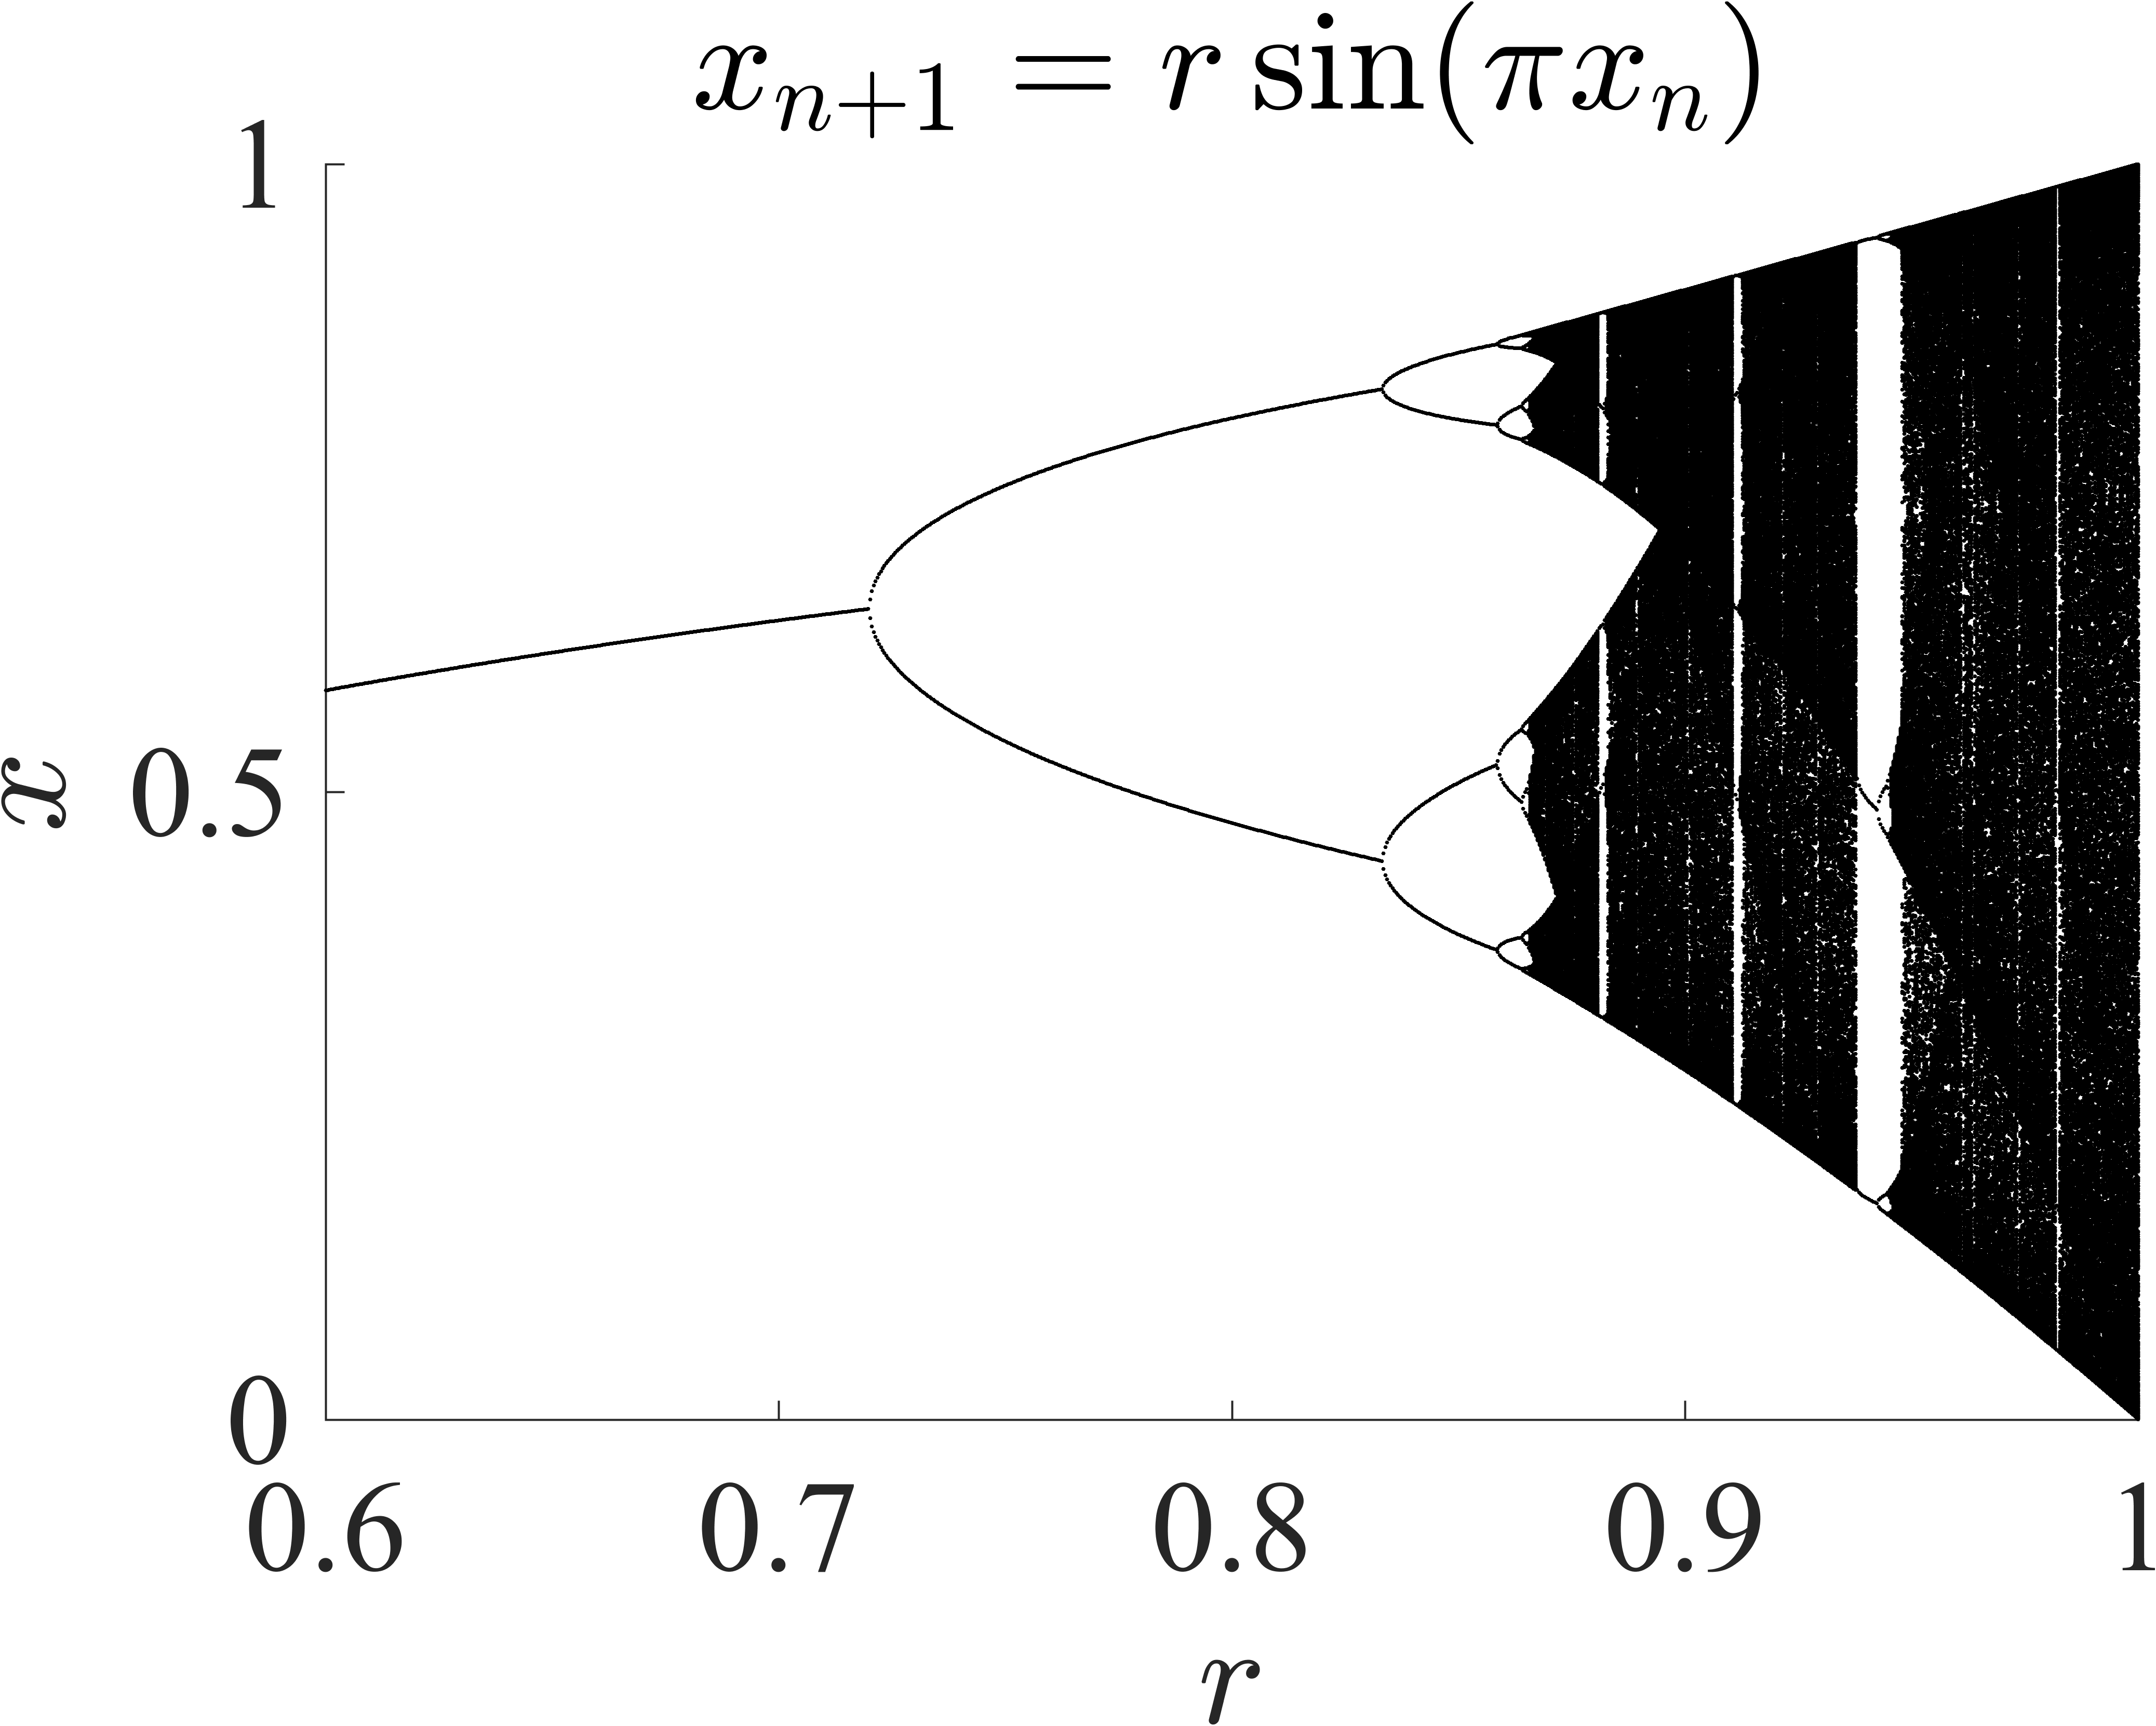
\includegraphics[width=8cm]{Sine_mapM.png}
\caption{Logistic Map and Sine Map}
\end{figure}

If we zoom into the figure, we see that there is no singular attractor after $r$ is above some critical value:
\begin{figure}[h]
\centering
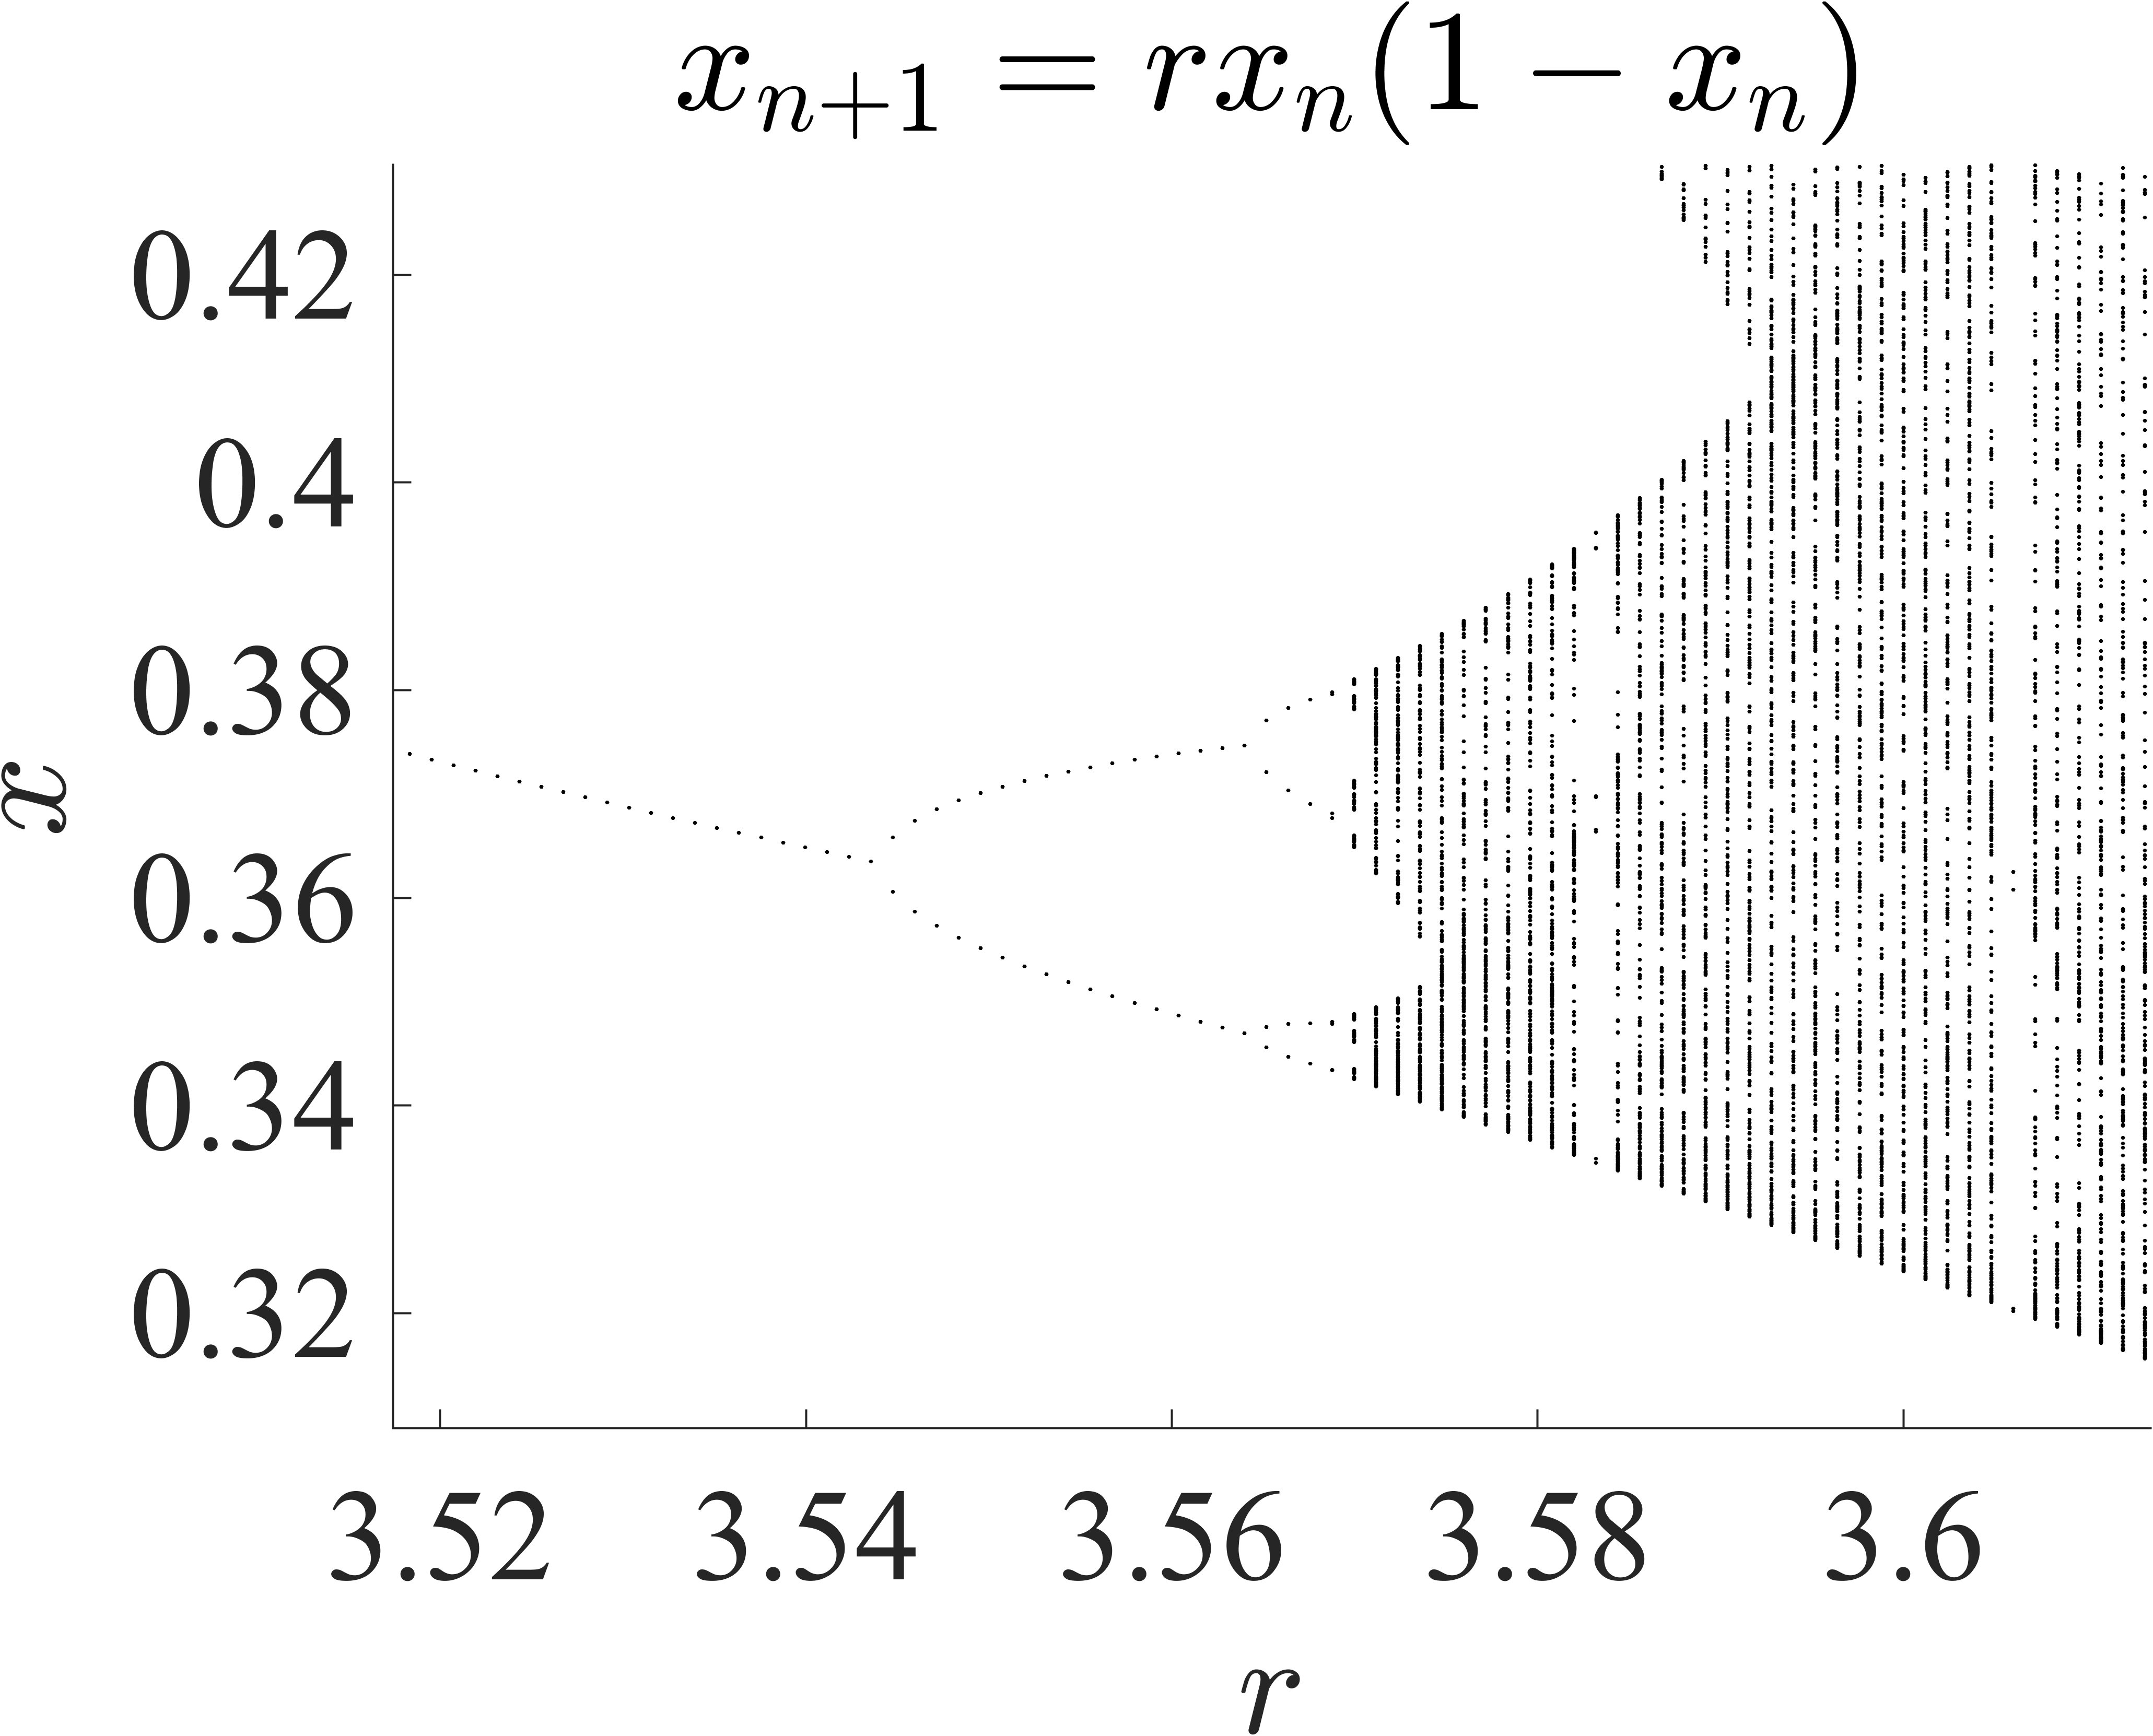
\includegraphics[width=8cm]{Logistic_map_zoom_in.png}
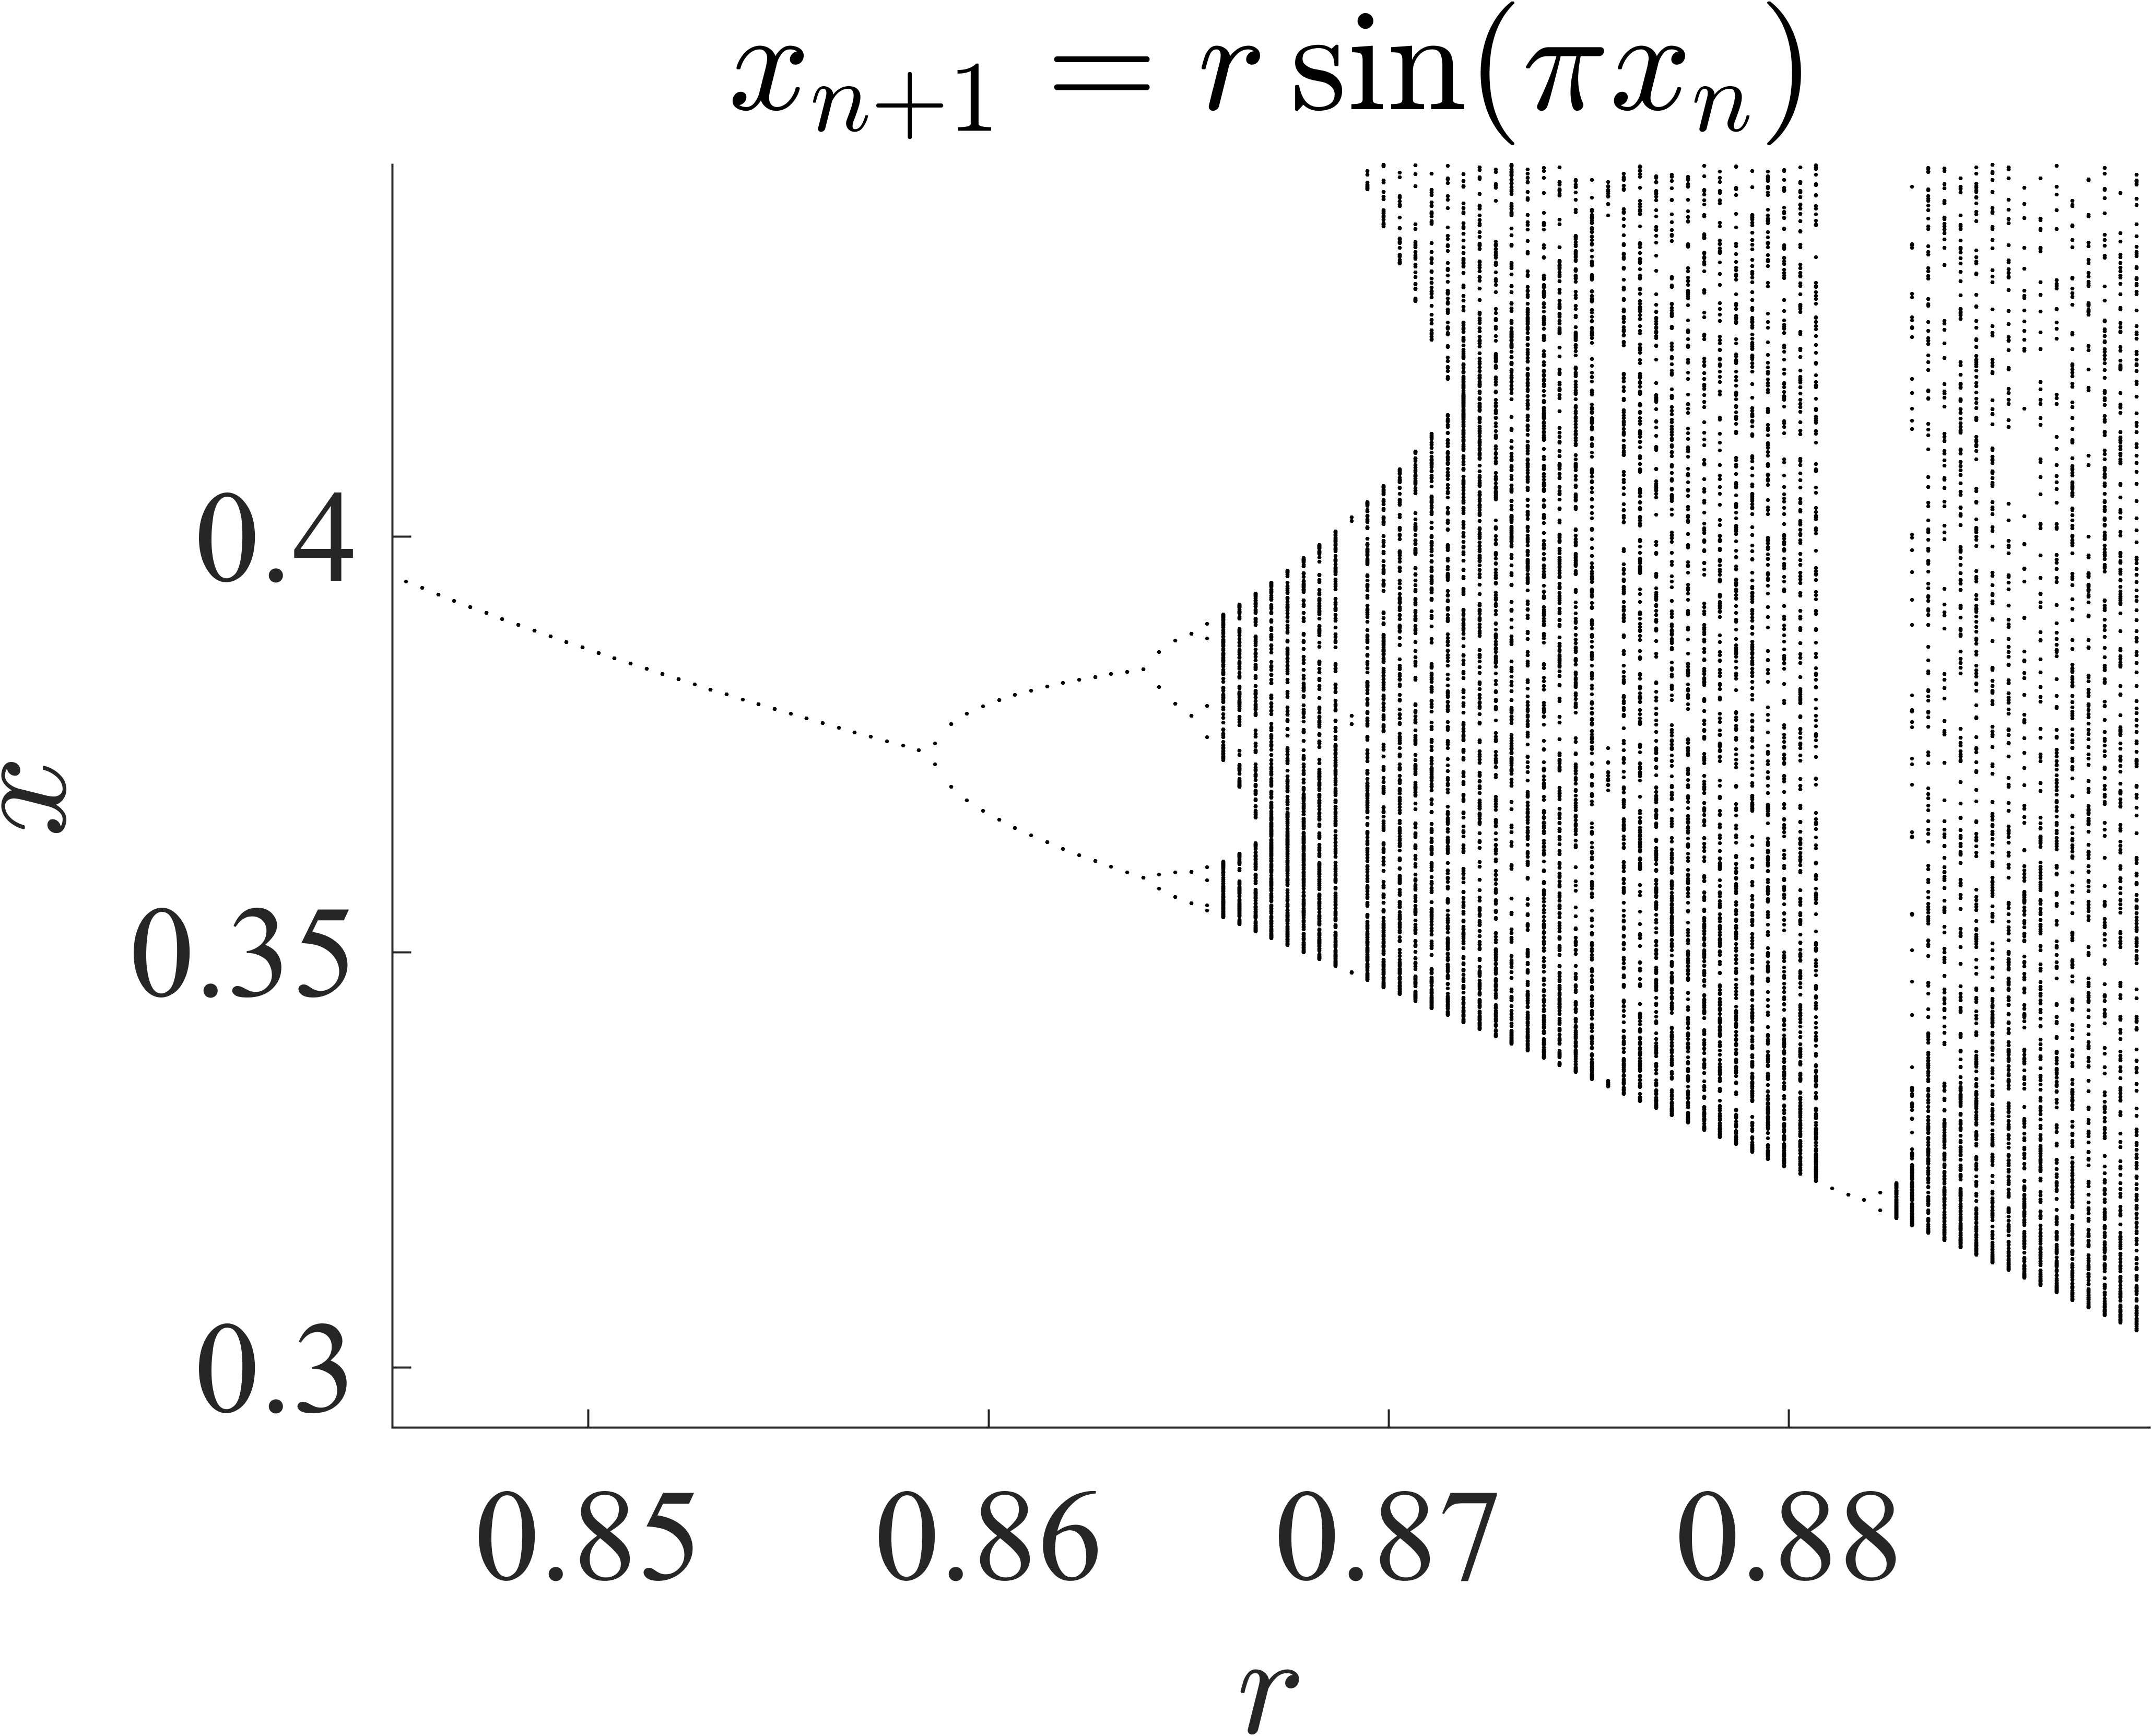
\includegraphics[width=8cm]{Sine_map_zoom_in.png}
\caption{Logistic Map and Sine Map }
\end{figure}

The attractor also has a complex and interesting structure in which there seem to be small vertical period windows that contain smaller version of the overall structure. If we zoom in to one of the period windows, we see the overall structure of the diagram reappear:
\begin{figure}[h]
\centering
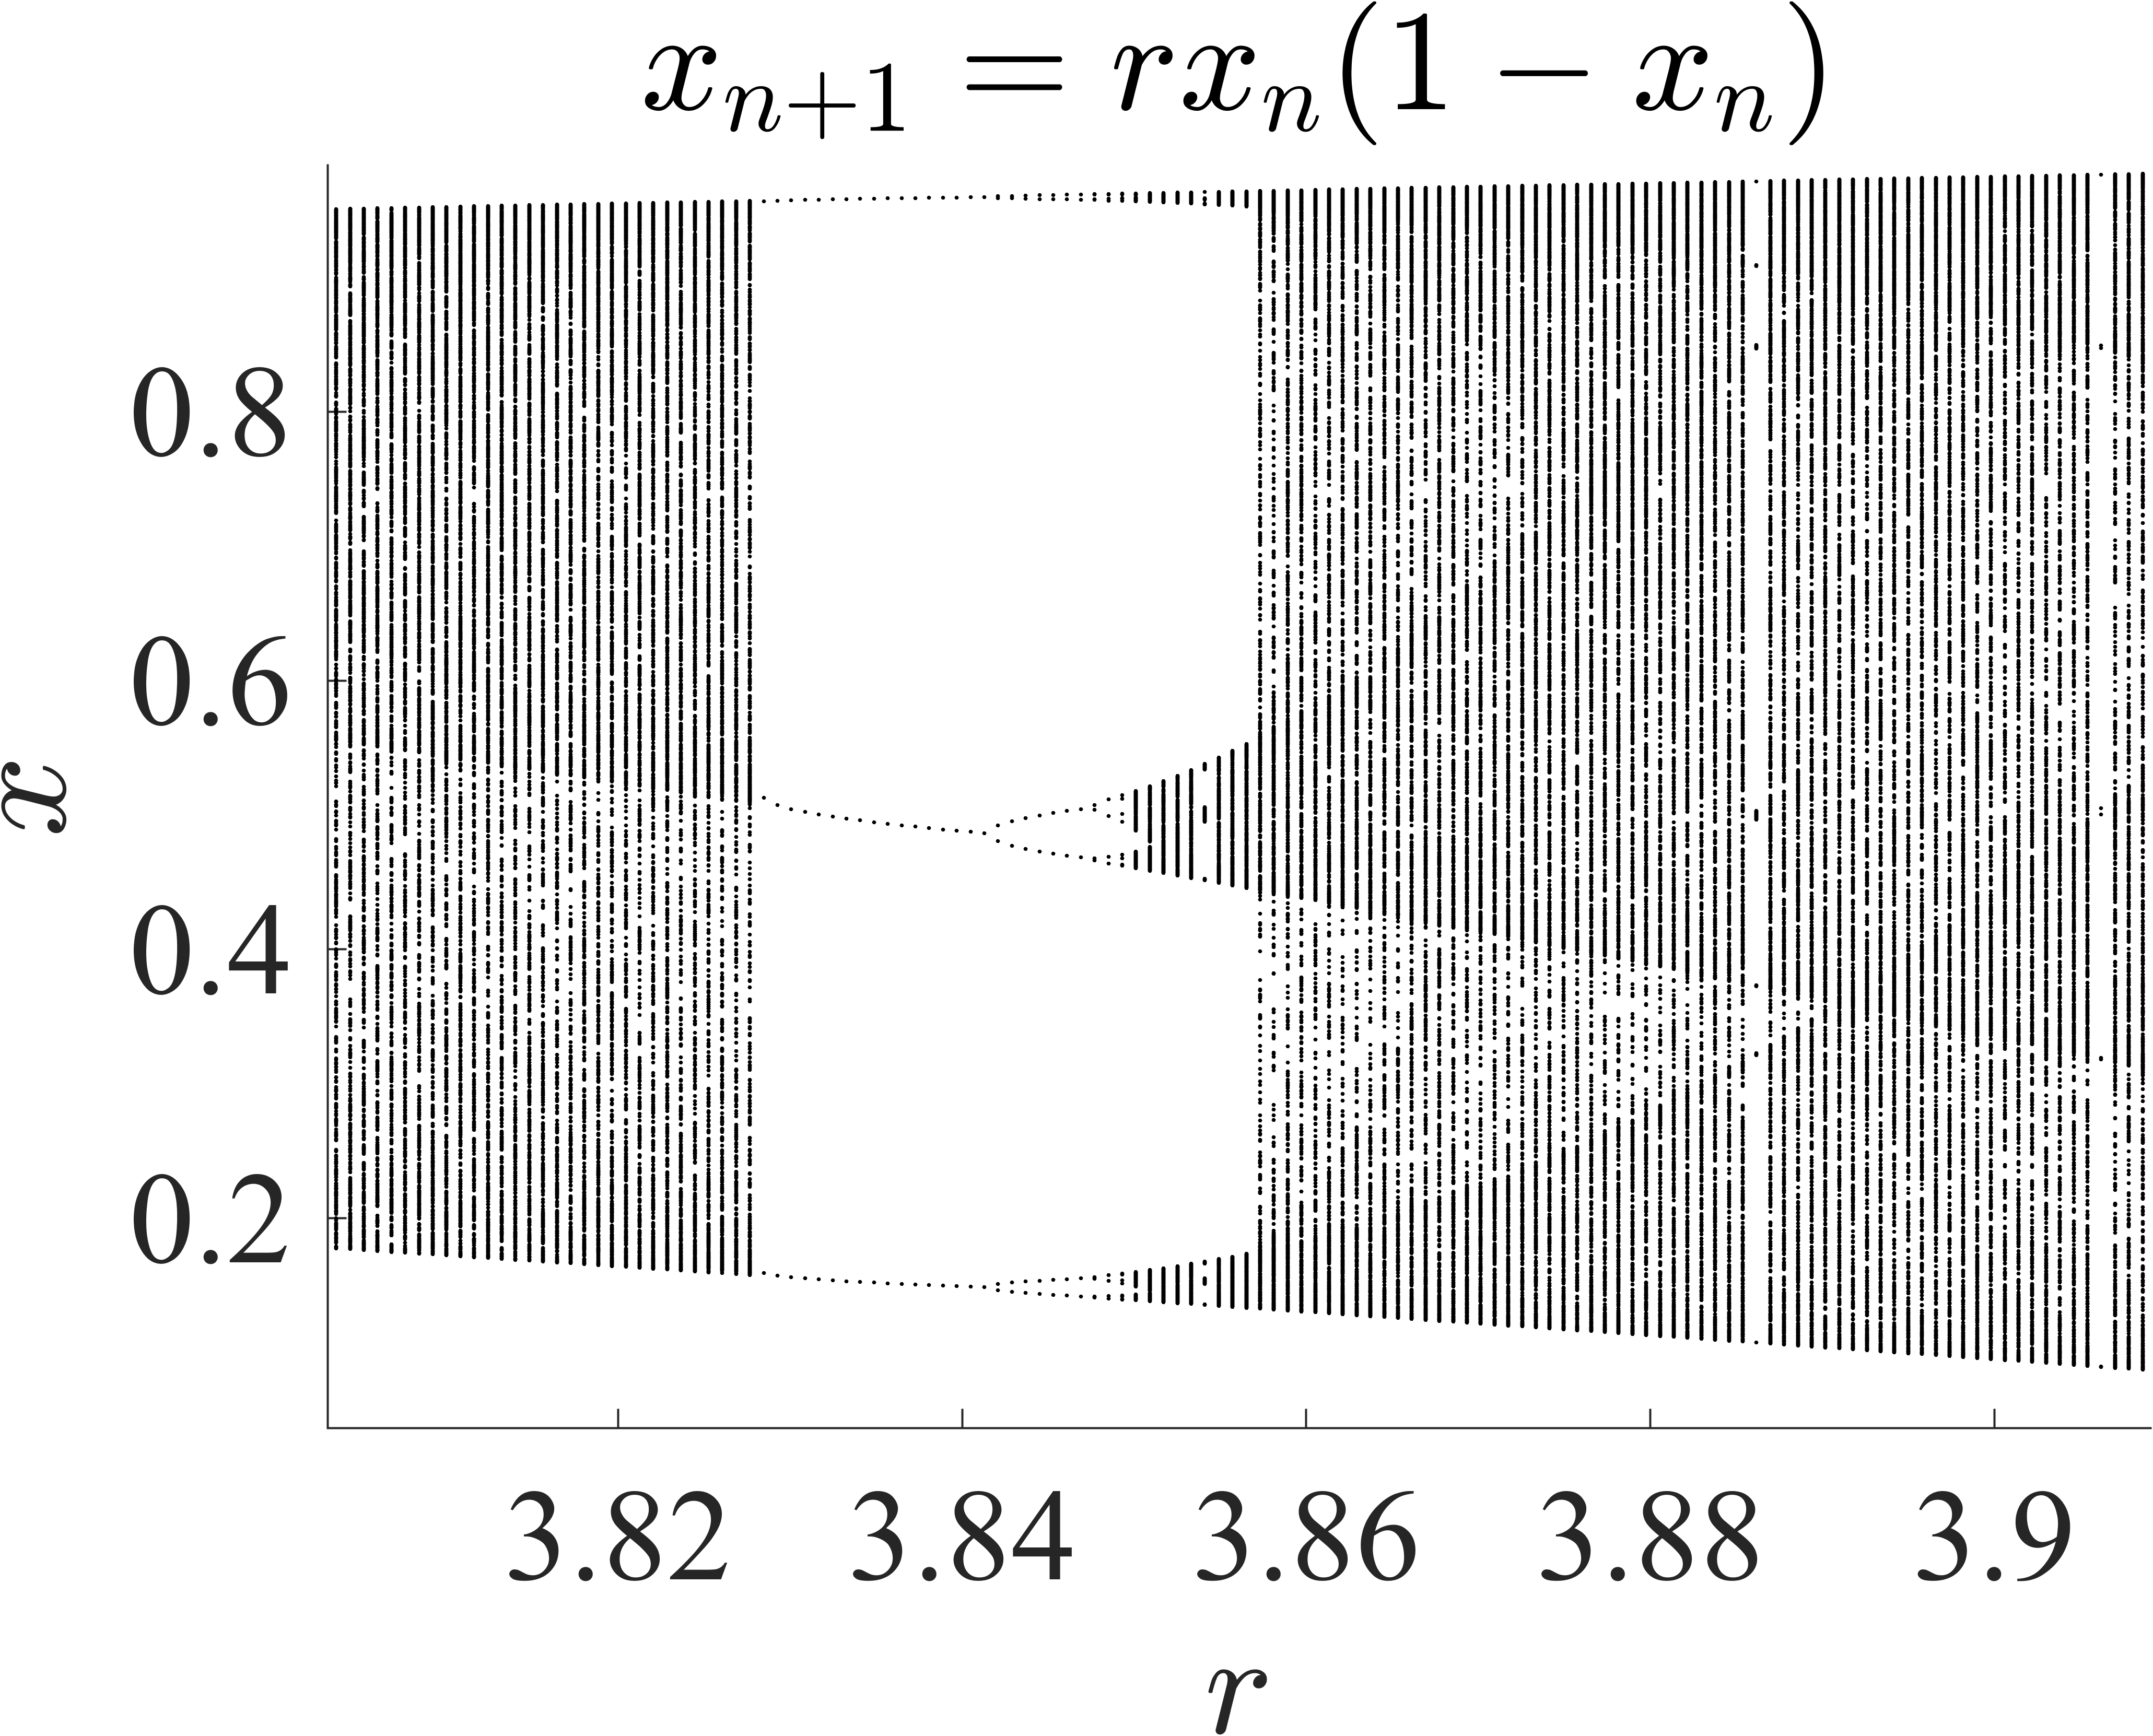
\includegraphics[width=8cm]{Logistic_map_PW.png}
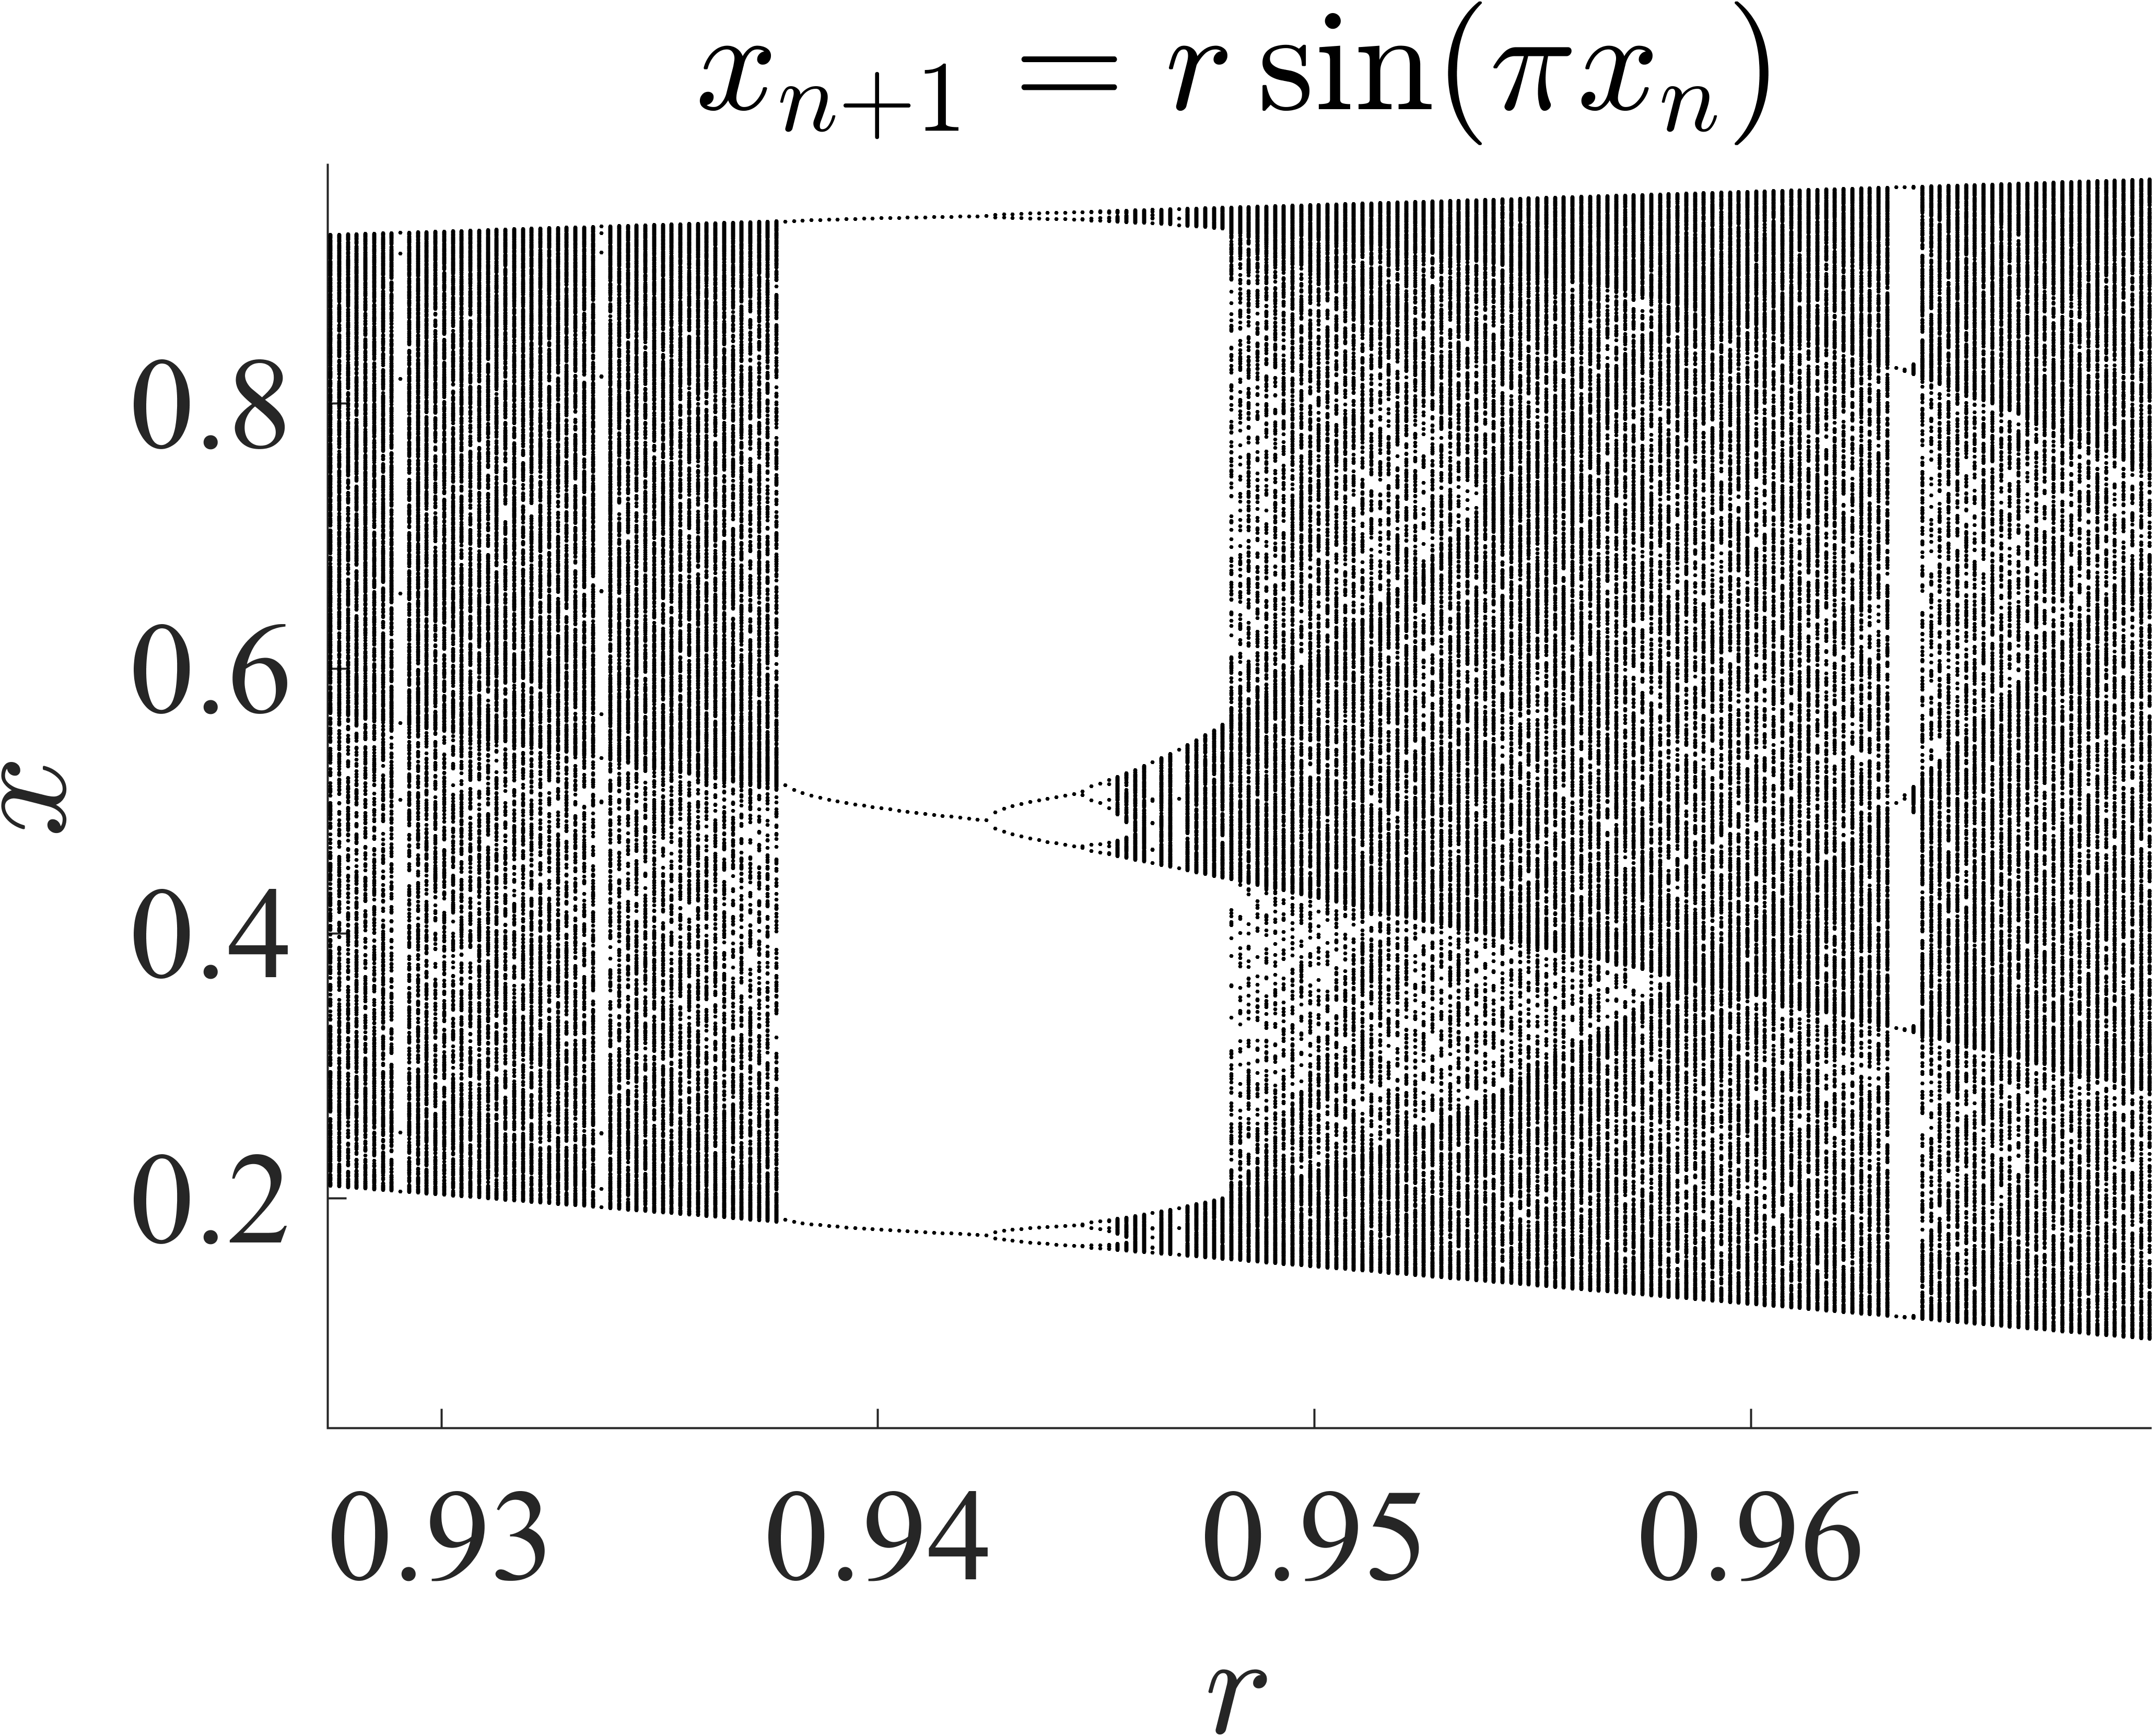
\includegraphics[width=8cm]{Sine_map_zoom_PW.png}
\caption{Logistic Map and Sine Map}
\end{figure}

I then adapted the code from the notes to calculate the values of $r$ where the period doubles for the logistic system, obtaining $r_1 = 3.0000$, $r_2=3.4498$,   $r_3 =  3.5443$, $r_4=    3.5649$, $r_5=    3.5690$. We know that from the Feigenbaum constant, we should expect that 
$$\delta = \lim_{n\rightarrow \infty} \frac{r_n - r_{n-1}}{r_{n+1} - r_n} = 4.669...$$
This means that the spacing of the period doublings should approach a regular pattern in which $\Delta_n / \Delta_{n+1} \rightarrow \delta$. With my values, I obtained a $\delta$ relatively closed to that known value. For $n = 2$, I got $\delta = 4.7597$. For $n = 3$, I got $\delta = 4.5812$, and for $n = 4$, I got  $\delta = 5.0263$. Increasing the number of periods and the numerical accuracy of my bifurcation detection would make my $\delta$ values better converge to the limit as $n$ increases.


\section*{Code}

\begin{lstlisting}{language=matlab}
% Kameel Khabaz
% CAAM 28200
% Homework 6 Lorenz Simulations

sigma = 10;
b = 8/3;
rH = (sigma * (sigma + b + 3))/(sigma - b -1);
r = rH - 1;
f = @myode;


figure()
close all;
hold on;
Cplus = [sqrt(b*(r-1)) sqrt(b*(r-1)) r-1];
initial_pos = [Cplus; Cplus + 1.* [1 1 1]];
for i = 1:2 %ength(initial_pos)
    scatter3(initial_pos(i,1),initial_pos(i,2),initial_pos(i,3),100,'filled','b');
    plot_solve(initial_pos(i,:),f,sigma, b, r)
end
scatter3(Cplus(1),Cplus(2),Cplus(3),100,'filled','r'); % C+ fixed point
set(gca,'FontSize',30,'FontName','times')
xlabel("$x$",'Interpreter','latex')
ylabel("$y$",'Interpreter','latex')
zlabel("$z$",'Interpreter','latex')
set(gcf,'Position',[0 0 700 500])
title("$r = " + r + ", r_H = " + rH+  ", \sigma = " + sigma + ", b = 8/3$",'Interpreter','latex')
%exportgraphics(gcf,"Lorenz_r" + r + ".png",'Resolution',600)
axis equal

%%
figure()
hold on
xlabel("$t$",'Interpreter','latex')
ylabel("$y$",'Interpreter','latex')
for i = 2 %ength(initial_pos)
    scatter(0,initial_pos(i,2),'filled','b');
    tspan = 0:.1:100;
    [~,sol] = ode45(@(t,y) myode(t,y,sigma, b, r),tspan,initial_pos(i,:));
    plot(tspan, sol(:,2),'k','LineWidth',.5);
end
set(gca,'FontSize',30,'FontName','times')

%% 2 neighboring trajectories 
sigma = 10;
b = 8/3;
rH = (sigma * (sigma + b + 3))/(sigma - b -1);
r = rH + 1;
f = @myode;


figure()
close all;
hold on;
delta = [.001 .001 .001];
Cplus = [sqrt(b*(r-1)) sqrt(b*(r-1)) r-1];
initial_pos = [Cplus; Cplus + delta];
cols = ['b' 'g']
solutions = {};
for i = 1:2 %ength(initial_pos)
    y0 = initial_pos(i,:);
    scatter3(initial_pos(i,1),initial_pos(i,2),initial_pos(i,3),100,'filled',cols(i));
    tspan = 0:.01:1000;
    opts = odeset('RelTol',1e-7,'AbsTol',1e-6);
    [~,sol] = ode45(@(t,y) myode(t,y,sigma, b, r),tspan,y0,opts);
    solutions{end+1} = sol;
    plot3(sol(:,1), sol(:,2),sol(:,3),'k','LineWidth',.5);
end

set(gca,'FontSize',30,'FontName','times')
xlabel("$x$",'Interpreter','latex')
ylabel("$y$",'Interpreter','latex')
zlabel("$z$",'Interpreter','latex')
set(gcf,'Position',[0 0 700 500])
title("$r = " + r + ", r_H = " + rH+  ", \sigma = " + sigma + ", b = 8/3$",'Interpreter','latex')
%exportgraphics(gcf,"Lorenz_r" + r + "2_trajectories.png",'Resolution',600)
axis equal

% Discrepancies plot
figure()
hold on;
discrep = vecnorm(solutions{1} - solutions{2},2,2);
normdiscrep = discrep ./ norm(delta);
normlogd = log(normdiscrep);
plot(tspan',normlogd,'k')
%{
% Now do the fit
linidcs = 1:find(tspan == 350);
f = fit(tspan(linidcs)',normlogd(linidcs),'poly1');
h = plot(f);
h.LineStyle = '--';
h.Color = "r";
h.LineWidth = 1.5;
legend(h,"$\lambda = "+ f.p1 + "$",'Interpreter','latex')
%}
xlabel("$t$",'Interpreter','latex')
ylabel("$\ln(\frac{||y(t) - x(t)||}{||\delta||})$",'Interpreter','latex')
title("$ ||\delta|| = " + norm(delta) + "$",'Interpreter','latex')
set(gca,'FontSize',30,'FontName','times')

%% Find local maxima
z = sol(:,3);
lmax = islocalmax(z,'MinProminence',.01);
map = [[0; z(lmax)] [z(lmax); 0] ];
map = map(2:end-1,:);
x = [max(map(:))/2:.1:max(map(:))];
y = x;
figure()
hold on
scatter(map(:,1),map(:,2),10,'r','filled')
plot(x, y,'k')
set(gca,'FontSize',30,'FontName','times')
xlabel("$z_n$",'Interpreter','latex')
ylabel("$z_{n+1}$",'Interpreter','latex')
title("Lorenz Map",'Interpreter','latex')
exportgraphics(gcf,"Lorenz_Map.png",'Resolution',600)
%% Make cobweb plot
ts = linspace(0,1,30);


f1 = figure()
hold on
scatter(map(:,1),map(:,2),10,'r','filled')
plot(x, y,'k')
set(gca,'FontSize',30,'FontName','times')


xlabel("$z_n$",'Interpreter','latex')
ylabel("$z_{n+1}$",'Interpreter','latex')
xlim([25 45])
ylim([25 45])
set(gca,'FontName','Times','FontSize',30)

Ns = zeros(length(ts),1);
No = 35;
Ns(1) = No;
for i = 2:length(ts)
    if mod(i,2) == 1
        [~,mini] = min(abs(map(:,1) - Ns(i-1)));
        Ns(i) = map(mini,2);
    else
        Ns(i) = Ns(i-1);
    end 
end
Ns_p1 = Ns(2:end);
Ns = Ns(1:end-1);
h = plot(Ns,Ns_p1,'b','LineWidth',1)
scatter(Ns,Ns_p1,'b')
scatter(No,No,75,'g','filled')
title("Lorenz Map",'Interpreter','latex')
legend(h,"$N_0 = " + No + "$",'Interpreter','latex')
exportgraphics(gcf,"Lorenz_map_cobwebs_No" + No + "_ld.png",'Resolution',600)


%% Maps and Period Doubling

logistic = @(r,x) r .* x .* (1 - x);
sine = @(r, x) r .* sin(pi .* x);
xo = 0.5;
rs = linspace(3.6,4,500);

% Do logistic
figure()
hold on
for i = 1:length(rs)
    logsols = recursion(logistic, rs(i), 100000, xo);
    scatter(repmat(rs(i), 1000,1), logsols(end-1000+1:end),1,'k','filled')
end 
set(gca,'FontName','Times','FontSize',30)
xlabel("$r$",'Interpreter','latex')
ylabel("$x$",'Interpreter','latex')
title("$x_{n+1} = rx_n(1-x_n)$",'Interpreter','latex')
%exportgraphics(gcf,"Logistic_map.png","Resolution",600)

%% Do sine map
figure()
hold on
rs = linspace(.9,1,500);
for i = 1:length(rs)
    logsols = recursion(sine, rs(i), 100000, xo);
    scatter(repmat(rs(i), 1000,1), logsols(end-1000+1:end),1,'k','filled');
end 
set(gca,'FontName','Times','FontSize',30)
xlabel("$r$",'Interpreter','latex')
ylabel("$x$",'Interpreter','latex')
title("$x_{n+1} = r\sin(\pi x_n)$",'Interpreter','latex')
%exportgraphics(gcf,"Sine_map.png","Resolution",600)

%% Calculating r of bifurcations, adapted from Strang notes
rs = linspace(2.8,3.57,10^4); % Increase spacing of r 
xs = linspace(0,1,10^4);
f_logistic = @(x,r) r*x.*(1 - x);
f_sine = @(x,r) r*sin(pi*x);

f{1} = @(x,r) f_logistic(x,r);
for j = 1:31
    f{j+1} = @(x,r) f{1}(f{j}(x,r),r);
end

new_period = 0;
rBifurcations = [];
for j = 1:length(rs)
    r = rs(j);
    % find fixed points and cycles (up to period 16)
    period = new_period;
    for p = 0:period
        step = 2^p;
        % find intersections
        sign_func = @(x) sign(f{step}(x,r) - x);
        signs = sign_func(xs);
        indices{p+1} = find(abs(diff(signs)) ~= 0); % indices corresponding to equilibrium for period 2^p
        indices{p+1} = sort(indices{p+1},'ascend');
        indices{p+1}(1) = []; % drop the equilibrium at 0
        % get stability
        stability = nan(size(indices{p+1}));
        for index_n = 1:length(indices{p+1})
            index = indices{p+1}(index_n);
            slope = (f{step}(xs(index+1),r) - f{step}(xs(index-1),r))/(xs(index+1) - xs(index - 1));
            stability(index_n) = abs(slope);
        end
        unstable{p+1} = indices{p+1}(stability > 1);
        stable{p+1} = indices{p+1}(stability < 1);
    end
    
    % check if we need higher period
    if length(unstable{period+1}) == length(indices{period+1})
        new_period = period+1;
        rBifurcations = [rBifurcations r];
    end
    % bound to avoid diverging
    new_period = min(new_period,7);
    
end

function sols = recursion(f, r, nsteps, xo)
    sols = nan(nsteps,1);
    sols(1) = xo;
    for i = 2:nsteps
        sols(i) = f(r, sols(i-1));
    end
end 

function dydt = myode(~,yvec,sigma, b, r)
    x = yvec(1);
    y = yvec(2);
    z = yvec(3);
    xdot = sigma * (y - x);
    ydot = r * x - y - x .* z;
    zdot = x .* y - b * z;
    dydt = [xdot; ydot; zdot];
end
\end{lstlisting}


\end{document}